\documentclass[journal,12pt,twocolumn]{IEEEtran}
%
\usepackage{setspace}
\usepackage{gensymb}
%\doublespacing
\singlespacing

%\usepackage{graphicx}
%\usepackage{amssymb}
%\usepackage{relsize}
\usepackage[cmex10]{amsmath}
%\usepackage{amsthm}
%\interdisplaylinepenalty=2500
%\savesymbol{iint}
%\usepackage{txfonts}
%\restoresymbol{TXF}{iint}
%\usepackage{wasysym}
\usepackage{amsthm}
\usepackage{iithtlc}
\usepackage{mathrsfs}
\usepackage{txfonts}
\usepackage{stfloats}
\usepackage{bm}
\usepackage{cite}
\usepackage{cases}
\usepackage{subfig}
%\usepackage{xtab}
\usepackage{longtable}
\usepackage{multirow}
%\usepackage{algorithm}
%\usepackage{algpseudocode}
\usepackage{enumitem}
\usepackage{mathtools}
\usepackage{tikz}
\usepackage{circuitikz}
\usepackage{verbatim}
\usepackage{tfrupee}
\usepackage[breaklinks=true]{hyperref}
%\usepackage{stmaryrd}
\usepackage{tkz-euclide} % loads  TikZ and tkz-base
\usetkzobj{all}
\usepackage{listings}
    \usepackage{color}                                            %%
    \usepackage{array}                                            %%
    \usepackage{longtable}                                        %%
    \usepackage{calc}                                             %%
    \usepackage{multirow}                                         %%
    \usepackage{hhline}                                           %%
    \usepackage{ifthen}                                           %%
  %optionally (for landscape tables embedded in another document): %%
    \usepackage{lscape}     
\usepackage{multicol}
\usepackage{chngcntr}
%\usepackage{enumerate}

%\usepackage{wasysym}
%\newcounter{MYtempeqncnt}
\DeclareMathOperator*{\Res}{Res}
%\renewcommand{\baselinestretch}{2}
\renewcommand\thesection{\arabic{section}}
\renewcommand\thesubsection{\thesection.\arabic{subsection}}
\renewcommand\thesubsubsection{\thesubsection.\arabic{subsubsection}}

\renewcommand\thesectiondis{\arabic{section}}
\renewcommand\thesubsectiondis{\thesectiondis.\arabic{subsection}}
\renewcommand\thesubsubsectiondis{\thesubsectiondis.\arabic{subsubsection}}

% correct bad hyphenation here
\hyphenation{op-tical net-works semi-conduc-tor}
\def\inputGnumericTable{}                                 %%

\lstset{
%language=C,
frame=single, 
breaklines=true,
columns=fullflexible
}
%\lstset{
%language=tex,
%frame=single, 
%breaklines=true
%}

\begin{document}
%


\newtheorem{theorem}{Theorem}[section]
\newtheorem{problem}{Problem}
\newtheorem{proposition}{Proposition}[section]
\newtheorem{lemma}{Lemma}[section]
\newtheorem{corollary}[theorem]{Corollary}
\newtheorem{example}{Example}[section]
\newtheorem{definition}[problem]{Definition}
%\newtheorem{thm}{Theorem}[section] 
%\newtheorem{defn}[thm]{Definition}
%\newtheorem{algorithm}{Algorithm}[section]
%\newtheorem{cor}{Corollary}
\newcommand{\BEQA}{\begin{eqnarray}}
\newcommand{\EEQA}{\end{eqnarray}}
\newcommand{\define}{\stackrel{\triangle}{=}}

\bibliographystyle{IEEEtran}
%\bibliographystyle{ieeetr}


\providecommand{\mbf}{\mathbf}
\providecommand{\pr}[1]{\ensuremath{\Pr\left(#1\right)}}
\providecommand{\qfunc}[1]{\ensuremath{Q\left(#1\right)}}
\providecommand{\sbrak}[1]{\ensuremath{{}\left[#1\right]}}
\providecommand{\lsbrak}[1]{\ensuremath{{}\left[#1\right.}}
\providecommand{\rsbrak}[1]{\ensuremath{{}\left.#1\right]}}
\providecommand{\brak}[1]{\ensuremath{\left(#1\right)}}
\providecommand{\lbrak}[1]{\ensuremath{\left(#1\right.}}
\providecommand{\rbrak}[1]{\ensuremath{\left.#1\right)}}
\providecommand{\cbrak}[1]{\ensuremath{\left\{#1\right\}}}
\providecommand{\lcbrak}[1]{\ensuremath{\left\{#1\right.}}
\providecommand{\rcbrak}[1]{\ensuremath{\left.#1\right\}}}
\theoremstyle{remark}
\newtheorem{rem}{Remark}
\newcommand{\sgn}{\mathop{\mathrm{sgn}}}
\providecommand{\abs}[1]{\left\vert#1\right\vert}
\providecommand{\res}[1]{\Res\displaylimits_{#1}} 
\providecommand{\norm}[1]{\left\lVert#1\right\rVert}
%\providecommand{\norm}[1]{\lVert#1\rVert}
\providecommand{\mtx}[1]{\mathbf{#1}}
\providecommand{\mean}[1]{E\left[ #1 \right]}
\providecommand{\fourier}{\overset{\mathcal{F}}{ \rightleftharpoons}}
%\providecommand{\hilbert}{\overset{\mathcal{H}}{ \rightleftharpoons}}
\providecommand{\system}{\overset{\mathcal{H}}{ \longleftrightarrow}}
	%\newcommand{\solution}[2]{\textbf{Solution:}{#1}}
\newcommand{\solution}{\noindent \textbf{Solution: }}
\newcommand{\cosec}{\,\text{cosec}\,}
\providecommand{\dec}[2]{\ensuremath{\overset{#1}{\underset{#2}{\gtrless}}}}
\newcommand{\myvec}[1]{\ensuremath{\begin{pmatrix}#1\end{pmatrix}}}
\newcommand{\mydet}[1]{\ensuremath{\begin{vmatrix}#1\end{vmatrix}}}
%\numberwithin{equation}{section}
\numberwithin{equation}{subsection}
%\numberwithin{problem}{section}
%\numberwithin{definition}{section}
\makeatletter
\@addtoreset{figure}{problem}
\makeatother

\let\StandardTheFigure\thefigure
\let\vec\mathbf
%\renewcommand{\thefigure}{\theproblem.\arabic{figure}}
\renewcommand{\thefigure}{\theproblem}
%\setlist[enumerate,1]{before=\renewcommand\theequation{\theenumi.\arabic{equation}}
%\counterwithin{equation}{enumi}


%\renewcommand{\theequation}{\arabic{subsection}.\arabic{equation}}

\def\putbox#1#2#3{\makebox[0in][l]{\makebox[#1][l]{}\raisebox{\baselineskip}[0in][0in]{\raisebox{#2}[0in][0in]{#3}}}}
     \def\rightbox#1{\makebox[0in][r]{#1}}
     \def\centbox#1{\makebox[0in]{#1}}
     \def\topbox#1{\raisebox{-\baselineskip}[0in][0in]{#1}}
     \def\midbox#1{\raisebox{-0.5\baselineskip}[0in][0in]{#1}}

\vspace{3cm}

\title{
	\logo{
Continuous Math
	}
}
\author{ G V V Sharma$^{*}$% <-this % stops a space
	\thanks{*The author is with the Department
		of Electrical Engineering, Indian Institute of Technology, Hyderabad
		502285 India e-mail:  gadepall@iith.ac.in. All content in this manual is released under GNU GPL.  Free and open source.}
	
}	
%\title{
%	\logo{Matrix Analysis through Octave}{\begin{center}\includegraphics[scale=.24]{tlc}\end{center}}{}{HAMDSP}
%}


% paper title
% can use linebreaks \\ within to get better formatting as desired
%\title{Matrix Analysis through Octave}
%
%
% author names and IEEE memberships
% note positions of commas and nonbreaking spaces ( ~ ) LaTeX will not break
% a structure at a ~ so this keeps an author's name from being broken across
% two lines.
% use \thanks{} to gain access to the first footnote area
% a separate \thanks must be used for each paragraph as LaTeX2e's \thanks
% was not built to handle multiple paragraphs
%

%\author{<-this % stops a space
%\thanks{}}
%}
% note the % following the last \IEEEmembership and also \thanks - 
% these prevent an unwanted space from occurring between the last author name
% and the end of the author line. i.e., if you had this:
% 
% \author{....lastname \thanks{...} \thanks{...} }
%                     ^------------^------------^----Do not want these spaces!
%
% a space would be appended to the last name and could cause every name on that
% line to be shifted left slightly. This is one of those "LaTeX things". For
% instance, "\textbf{A} \textbf{B}" will typeset as "A B" not "AB". To get
% "AB" then you have to do: "\textbf{A}\textbf{B}"
% \thanks is no different in this regard, so shield the last } of each \thanks
% that ends a line with a % and do not let a space in before the next \thanks.
% Spaces after \IEEEmembership other than the last one are OK (and needed) as
% you are supposed to have spaces between the names. For what it is worth,
% this is a minor point as most people would not even notice if the said evil
% space somehow managed to creep in.



% The paper headers
%\markboth{Journal of \LaTeX\ Class Files,~Vol.~6, No.~1, January~2007}%
%{Shell \MakeLowercase{\textit{et al.}}: Bare Demo of IEEEtran.cls for Journals}
% The only time the second header will appear is for the odd numbered pages
% after the title page when using the twoside option.
% 
% *** Note that you probably will NOT want to include the author's ***
% *** name in the headers of peer review papers.                   ***
% You can use \ifCLASSOPTIONpeerreview for conditional compilation here if
% you desire.




% If you want to put a publisher's ID mark on the page you can do it like
% this:
%\IEEEpubid{0000--0000/00\$00.00~\copyright~2007 IEEE}
% Remember, if you use this you must call \IEEEpubidadjcol in the second
% column for its text to clear the IEEEpubid mark.



% make the title area
\maketitle

\newpage

\tableofcontents

\bigskip

\renewcommand{\thefigure}{\theenumi}
\renewcommand{\thetable}{\theenumi}
%\renewcommand{\theequation}{\theenumi}

%\begin{abstract}
%%\boldmath
%In this letter, an algorithm for evaluating the exact analytical bit error rate  (BER)  for the piecewise linear (PL) combiner for  multiple relays is presented. Previous results were available only for upto three relays. The algorithm is unique in the sense that  the actual mathematical expressions, that are prohibitively large, need not be explicitly obtained. The diversity gain due to multiple relays is shown through plots of the analytical BER, well supported by simulations. 
%
%\end{abstract}
% IEEEtran.cls defaults to using nonbold math in the Abstract.
% This preserves the distinction between vectors and scalars. However,
% if the journal you are submitting to favors bold math in the abstract,
% then you can use LaTeX's standard command \boldmath at the very start
% of the abstract to achieve this. Many IEEE journals frown on math
% in the abstract anyway.

% Note that keywords are not normally used for peerreview papers.
%\begin{IEEEkeywords}
%Cooperative diversity, decode and forward, piecewise linear
%\end{IEEEkeywords}



% For peer review papers, you can put extra information on the cover
% page as needed:
% \ifCLASSOPTIONpeerreview
% \begin{center} \bfseries EDICS Category: 3-BBND \end{center}
% \fi
%
% For peerreview papers, this IEEEtran command inserts a page break and
% creates the second title. It will be ignored for other modes.
%\IEEEpeerreviewmaketitle

\begin{abstract}
This book provides a computational approach to continuous mathematics based on the NCERT textbooks from Class 6-12.  Links to sample Python codes are available in the text.  
\end{abstract}
Download python codes using 
\begin{lstlisting}
svn co https://github.com/gadepall/school/trunk/ncert/continuous/codes
\end{lstlisting}

%\section{Triangle}
%%\subsection{Construction Examples}
%%\input{./triangle/triangle_const_examples.tex}
%%\subsection{Construction Exercises}
%%\input{./triangle/triangle_const_exercises.tex} 
%\subsection{Triangle Examples}
%\input{./triangle/tri_exam.tex} 
%\subsection{Triangle Exercises}
%\input{./triangle/tri_geo.tex} 
%%
%\section{Quadrilateral}
%%\subsection{Construction Examples}
%%\renewcommand{\theequation}{\theenumi}
\begin{enumerate}[label=\arabic*.,ref=\thesubsection.\theenumi]
\numberwithin{equation}{enumi}

\item Draw $ABCD$ with $AB=a=4.5, BC  =b=5.5, CD =c= 4, AD =d=6$ and $AC=e = 7$.
\\
\solution Fig. \ref{fig:quad_ex} shows a rough sketch of $ABCD$. Letting
\begin{align}
\label{eq:tri_basic_new}
\vec{C} = \myvec{p\\q}, \vec{A} = \myvec{0\\0}, \vec{B} = \myvec{a\\0}
\end{align}
%
it is trivial to sketch $\triangle ABC$ from  Problem \ref{prob:tri}.
%
$\triangle ACD$ is can be obtained by rotating an equivalent triangle with $AC$ on
the $x$-axis by an angle $\theta$ with
\begin{align}
\label{eq:tri_basic_rot}
\vec{D} = \myvec{h\\k}, \vec{A} = \myvec{0\\0}, \vec{C} = \myvec{e\\0}
\end{align}
%
and
\begin{align}
\label{eq:tri_rot_ang}
\cos \theta = \frac{a^2+e^2-b^2}{2ae}
\\
\sin \theta = \sqrt{1-\cos^2\theta}
\end{align}
%
The coordinates of the rotated triangle $ACD$ are
\begin{align}
\label{eq:tri_rot_trans}
\vec{D} = \vec{P}\myvec{h\\k}
\\
\vec{A} = \vec{P}\myvec{0\\0}
\\
\vec{C} = \vec{P}\myvec{e\\0}
\end{align}
%
where 
\begin{align}
\label{eq:tri_rot_mat}
\vec{P} = \myvec{\cos\theta & -\sin \theta\\ \sin \theta & \cos \theta}
\end{align}
\begin{figure}[!ht]
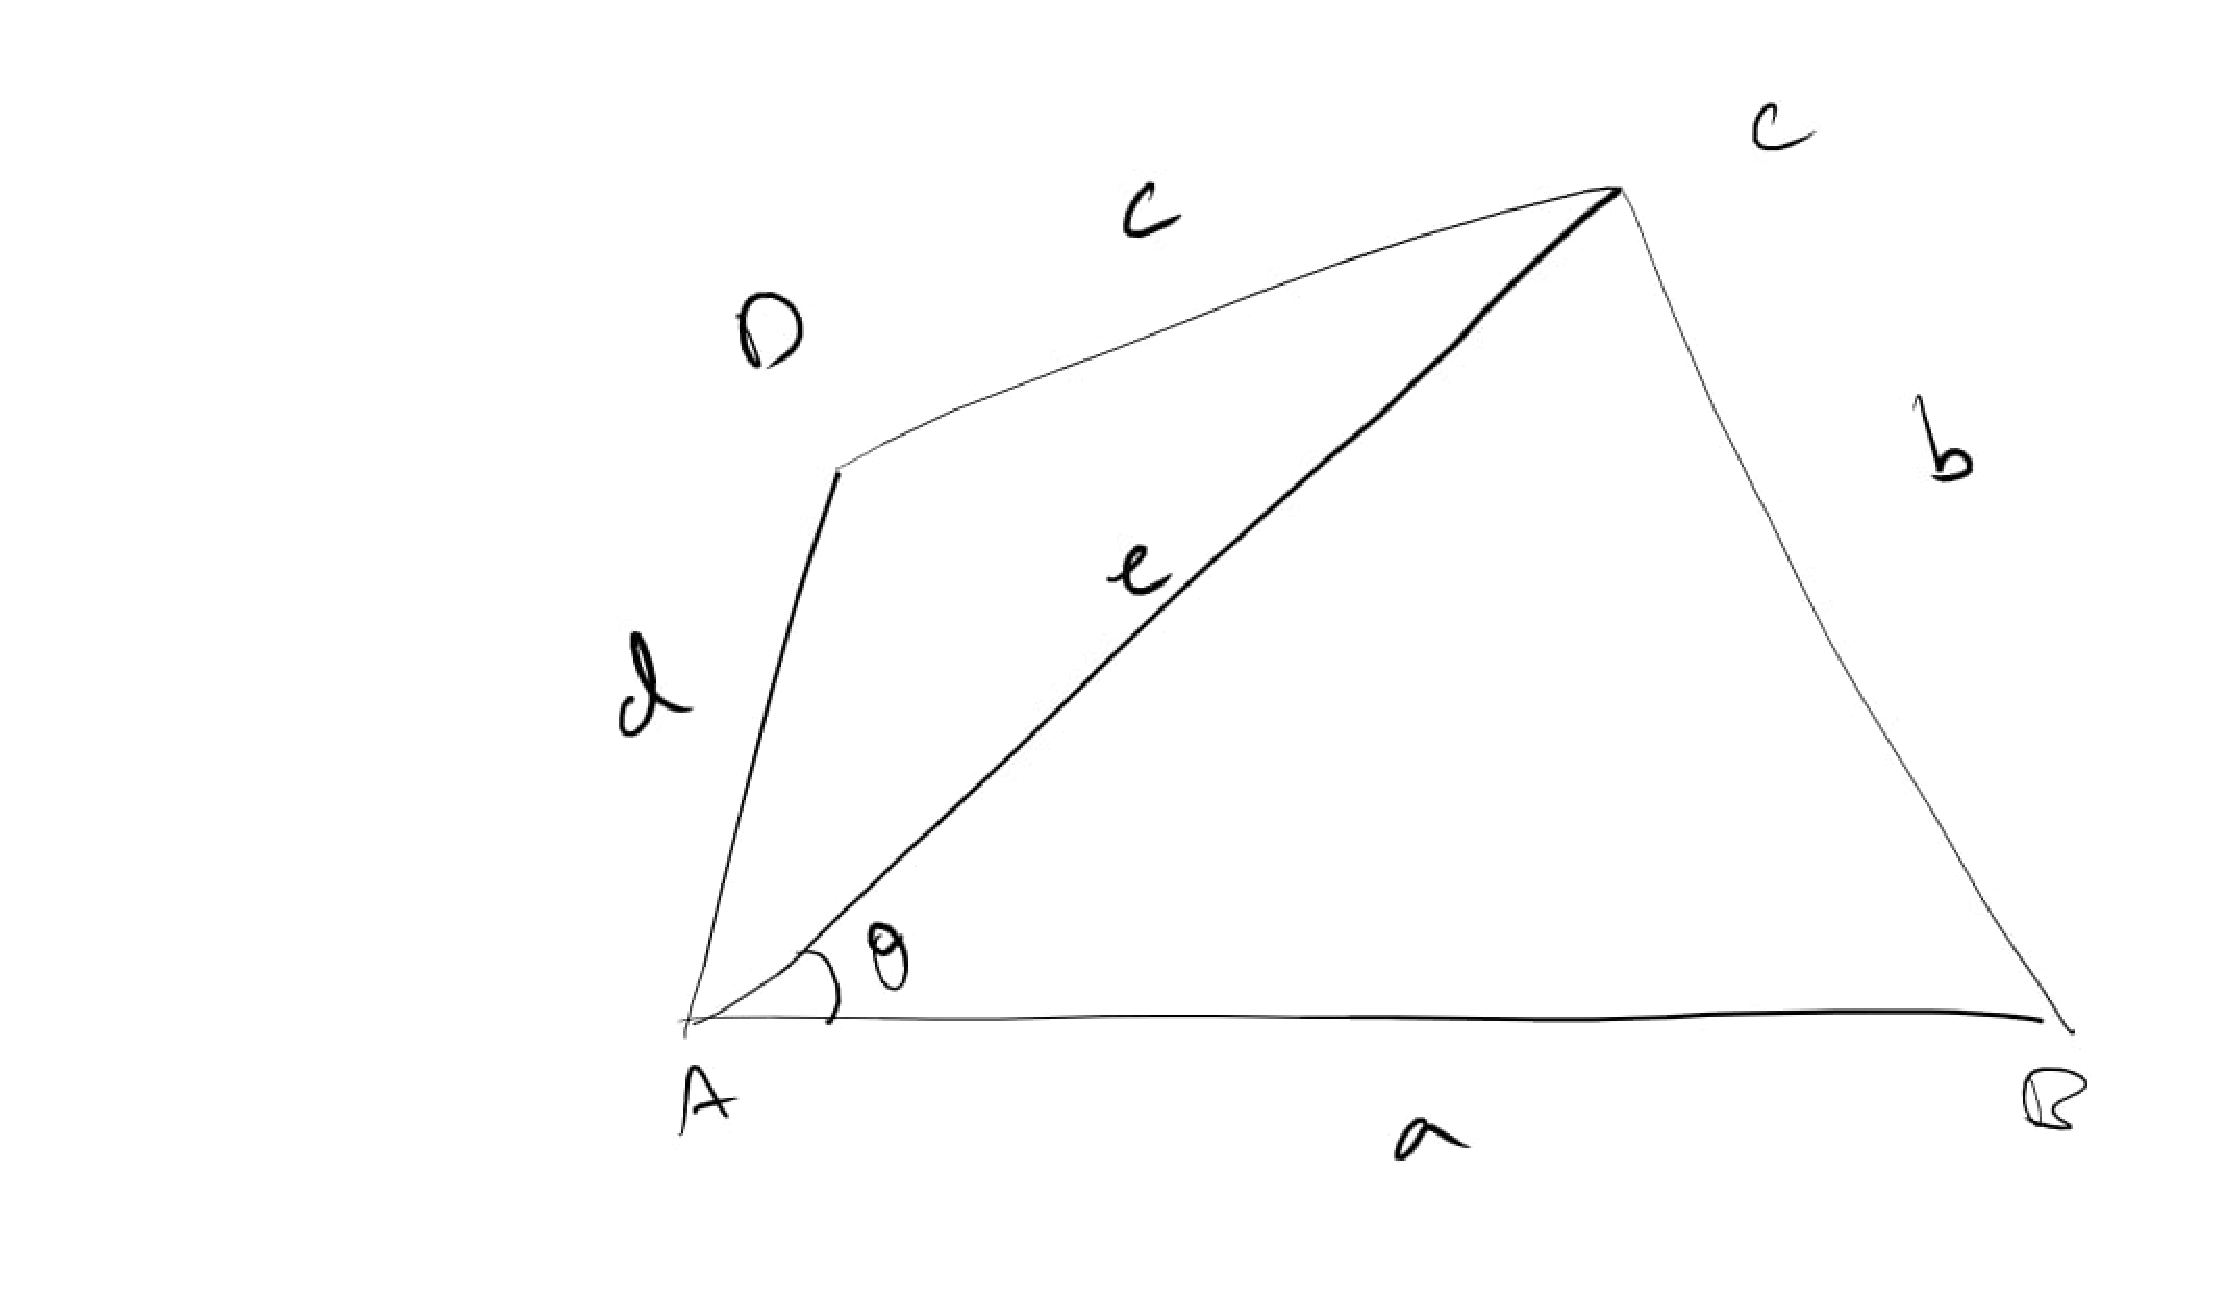
\includegraphics[width=\columnwidth]{./constructions/figs/quad_ex.eps}
\caption{}
\label{fig:quad_ex}
\end{figure}
The following code plots quadrilateral $ABCD$ in Fig. \ref{fig:quad}
\begin{lstlisting}
codes/draw_quad.py
\end{lstlisting}
\begin{figure}[!ht]
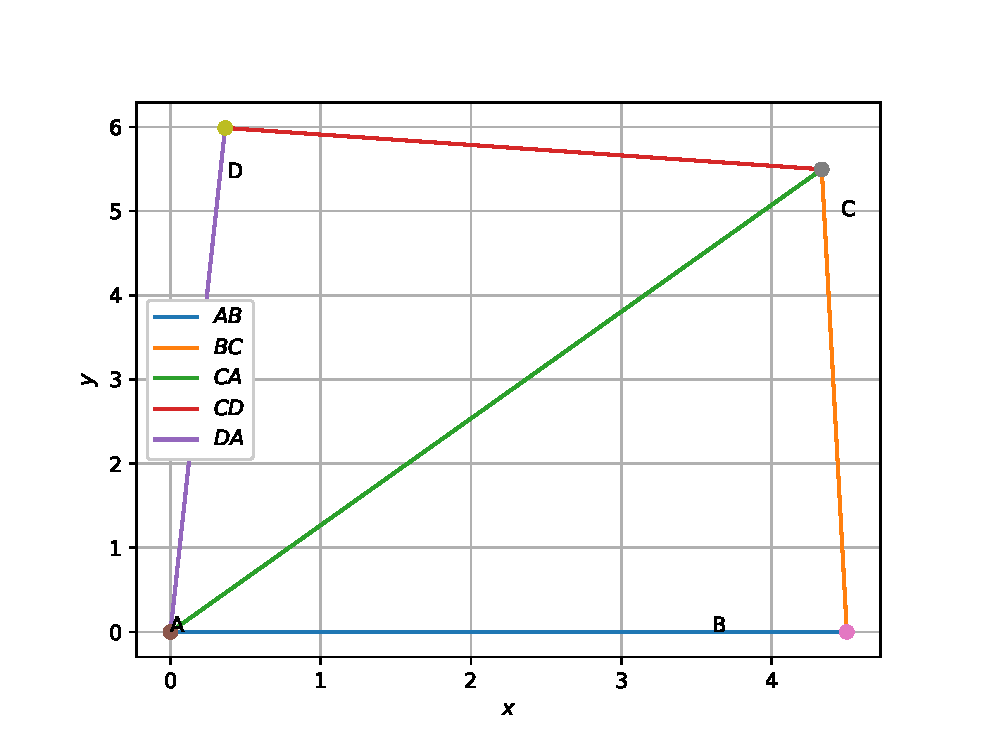
\includegraphics[width=\columnwidth]{./constructions/figs/quad.eps}
\caption{}
\label{fig:quad}
\end{figure}
\item Draw the parallelogram $MORE$ with $OR = 6, RE = 4.5$ and $EO=7.5$.
\\
\solution
Diagonals of a parallelogram bisect each other.  Opposite sides of a parallelogram are equal and parallel
.
\item Construct a kite $EASY$ if $AY = 8, EY = 4$ and $SY = 6$.
\\
\solution The diagonals of a kite are perpendicular to each other.
\item Draw the rhombus $BEST$ with $BE = 4.5$ and $ET = 6$. 
\\
\solution Diagonals of a rhombus bisect each other at right angles.


\end{enumerate}
%
 
%%\subsection{Construction Exercises}
%%\renewcommand{\theequation}{\theenumi}
\begin{enumerate}[label=\arabic*.,ref=\thesubsection.\theenumi]
\numberwithin{equation}{enumi}


\item Construct a quadrilateral $ABCD$ such that $AB=5, \angle A = 50\degree, AC = 4, BD = 5$ and $AD = 6$.
\item Construct $PQRS$ where $PQ = 4, QR = 6, RS = 5, PS = 5.5$ and $PR = 7$.
\item Draw $JUMP$ with $JU = 3.5, UM=4, MP = 5, PJ =4.5$ and $PU = 6.5$
\item Construct a quadrilateral $ABCD$ such that $BC=4.5,  AC = 5.5, CD = 5, BD = 7$ and $AD = 5.5$.
\item Can you construct a quadrilateral $PQRS$ with $PQ=3, RS=3, PS=7.5, PR=8$ and $SQ=4$?
\item Construct $LIFT$ such that $LI = 4, IF = 3, TL = 2.5, LF = 4.5, IT=4$.
\item Draw $GOLD$ such that $OL=7.5, GL=6, GD=6, LD = 5, OD = 10$.
\item DRAW rhombus $BEND$ such that $BN = 5.6$, $DE = 6.5$.
\item construct a quadrilateral MIST where $MI = 3.5, IS = 6.5, \angle M = 75 \degree, \angle I = 105 \degree$ and $\angle S = 120 \degree$.
\item Can you construct the above quadrilateral MIST if $\angle M = 100 \degree$ instead of $75 \degree$.
\item Can you constrcut the quadrilateral PLAN if $PL = 6, LA = 9.5, \angle P = 75 \degree, \angle L = 150 \degree$ and $\angle A = 140 \degree$?
\item Construct $MORE$ where $MO = 6, OR = 4.5, \angle M = 60 \degree, \angle O = 105 \degree, \angle R = 105 \degree$.
\item Construct $PLAN$ where $PL = 4, LA = 6.5, \angle P = 90 \degree, \angle A = 110\degree$ and $\angle N = 85\degree$.
\item Constrcut parallelogram $HEAR$ where $HE = 5, EA = 6, \angle R = 85 \degree$.
\item Draw  rectangle $OKAY$ with $OK = 7$ and $KA = 5$.
\item Construct $ABCd $, where $AB = 4, BC = 5, Cd = 6.5, \angle B = 105 \degree$ and $\angle C = 80\degree$.
\item Construct $DEAR$ with $DE = 4, EA = 5, AR = 4.5, \angle E = 60 \degree$ and $\angle A = 90 \degree$.\item Construct $TRUE$ with $TR = 3.5, RU = 3, UE = 4 \angle R = 75\degree$ and $\angle U = 120\degree$.
\item Draw a square of side 4.5.

\item Can you construct a rhombus $ABCD$ with $AC = 6$ and $BD = 7$?
\item Draw a square $READ$ with $RE = 5.1$.
\item Draw a rhombus who diagonals are $5.2$ and $6.4$.
\item Draw a rectangle with adjacent sides $5$ and $4$.
\item Draw a parallelogram $OKAY$ with $OK = 5.5$ and $KA = 4.2$.


\end{enumerate}
%
 
%\subsection{Quadrilateral Examples}
%\input{./quad/quad_geo_exam.tex} 
%\subsection{Quadrilateral Geometry}
%\input{./quad/quad_geo.tex} 
%%
%\section{Line}
%\subsection{Geometry: Examples}
%\input{./line/line_exam.tex}
%\subsection{Linear Inequalities: Examples}
%\input{./line/lineaeqn_exam.tex}
%\subsection{Linear Programing: Examples}
%\input{./line/lp_exam.tex}
%\subsection{Matrix Examples}
%\input{./line/matrix_exam.tex}
%\subsection{Complex Numbers}
%\input{./line/complex.tex}
%\subsection{Points and Vectors}
%\renewcommand{\theequation}{\theenumi}
\begin{enumerate}[label=\arabic*.,ref=\thesubsection.\theenumi]
\numberwithin{equation}{enumi}
\item Find the distance between the following pairs of points
\begin{enumerate}
\item 
\begin{align}
\myvec{2\\3}, \myvec{4\\1}
\end{align}
\item 
\begin{align}
\myvec{-5\\7}, \myvec{-1\\3}
\end{align}
\item 
\begin{align}
\myvec{a\\b}, \myvec{-1\\b}
\end{align}
\end{enumerate}
\item Find the distance between the points 
\begin{align}
\myvec{0\\0}, \myvec{36\\15}
\end{align}
%
\item A town B is located 36km east and 15 km north of the town A.  How would you find the distance from town A to town B without actually measuring it?
\item Determine if the points 
\begin{align}
\myvec{1\\5}, \myvec{2\\3}, \myvec{-2\\-11}
\end{align}
%
are collinear.	
\item Check whether 
\begin{align}
\myvec{5\\-2}, \myvec{6\\4}, \myvec{7\\-2}
\end{align}
are the vertices of an isosceles triangle.
\item Name the type of quadrilateral formed, if any, by the following points, and give reasons for your answer.
\begin{enumerate}
\item 
\begin{align}
\myvec{-1\\-2}, \myvec{1\\0},
\myvec{-1\\2}, \myvec{-3\\0}
\end{align}
\item 
\begin{align}
\myvec{-3\\5}, \myvec{3\\1},
\myvec{0\\3}, \myvec{-1\\-4}
\end{align}
\item 
\begin{align}
\myvec{4\\5}, \myvec{7\\6},
\myvec{4\\3}, \myvec{1\\2}
\end{align}
\item Find the point on the $x$-axis which is equidistant from 
\begin{align}
\myvec{2\\-5}, \myvec{-2\\9},
\end{align}
\item Find the alues of $y$ for which the distance between the points 
\begin{align}
\vec{P} = \myvec{2\\-3}, \vec{Q} = \myvec{10\\y}
\end{align}
is 10 units.
\end{enumerate}
\end{enumerate}
%

%\subsection{Points on a Line}
%\input{./line/section.tex}
%\subsection{Lines and Planes}
%\input{./line/line_equation.tex}
%\subsection{Matrix Exercises}
%\input{./line/matrix_exer.tex}
%\subsection{Determinants}
%\input{./line/determinants.tex}
%\subsection{Linear Inequalities: Exercises}
%\input{./line/lineaeqn_exer.tex}
%\subsection{Linear Programing: Exercises}
%\input{./line/lp_exer.tex}
%
%%\subsection{Examples: Applications}
%%\input{./line/line_app.tex}
%\subsection{Miscellaneous}
%\input{./line/line_misc.tex}
%
%\section{Circle}
%%\subsection{Construction Examples}
%%\input{./circle/circle_examples.tex} 
%%\subsection{Construction Exercises}
%%\input{./circle/circle_exer.tex} 
%\subsection{Circle Geometry Examples}
%\renewcommand{\theequation}{\theenumi}
\begin{enumerate}[label=\arabic*.,ref=\thesubsection.\theenumi]
\numberwithin{equation}{enumi}
\item 
\end{enumerate}
 
%\subsection{Circle Geometry Exercises}
%\renewcommand{\theequation}{\theenumi}
\begin{enumerate}[label=\arabic*.,ref=\thesubsection.\theenumi]
\numberwithin{equation}{enumi}
\item Find the coordinates of a point $\vec{A}$, where $AB$ is the diameter of a circle whose centre is \myvec{2,-3} and $\vec{B} = \myvec{1\\4}$.
\item Find the centre $O$f a circle passing through the points \myvec{6\\-6}, \myvec{3\\-7} and  \myvec{3\\3}.
\item Find the locus of all the unit vectors in the xy-plane.
%
\item $ABCD$ is a cyclic quadrilateral in which $AC$ and $BD$ are its diagonals. If $\angle DBC = 55\degree$ and $\angle BAC = 45\degree$, find $\angle BCD$
%
\item Two circles of radii 5 cm and 3 cm intersect at two points and the distance between their centres is 4 cm. Find the length of the common chord.
%
%
\item  A,B and C are three points on a circle with centre $O$ such that $\angle BOC = 30\degree $ and $ \angle AOB = 60\degree$. If D is a point on the circle other than the arc ABC, find $\angle ADC$.
%
\item $ \angle PQR = 100\degree$, where $P, Q$ and R are
points on a circle with centre $O$. Find $\angle OPR$.
\item $A, B, C, D$ are points on a circle such that $ \angle ABC = 69\degree, \angle ACB = 31\degree$, find
$\angle BDC$.
\item $A, B, C$ and $D$ are four points on a
circle. $AC$ and $BD$ intersect at a point $E$ such
that $\angle BEC = 130\degree$ and $\angle ECD = 20\degree$. Find $\angle BAC$.
\item $ABCD$ is a cyclic quadrilateral whose diagonals intersect at a point $E$. If $\angle DBC = 70\degree,
\angle BAC$ is $30\degree$, find $\angle BCD$. Further, if $AB = BC$, find $\angle ECD$.
%
\item Two chords $AB$ and $CD$ of lengths 5 cm and 11 cm respectively of a circle are parallel
to each other and are on opposite sides of its centre. If the distance between $AB$ and
$CD$ is 6 cm, find the radius of the circle.
\item The lengths of two parallel chords of a circle are 6 cm and 8 cm. If the smaller chord is
at distance 4 cm from the centre, what is the distance of the other chord from the
centre?
%
\item A tangent $PQ$ at a point $P$ of a circle of radius 5 cm meets a line through the centre $O$ at a point $Q$ so that $OQ =$ 12 cm. Find the length of $PQ$.
%
\item $PQ$ is a chord of length 8 cm of a circle of radius 5 cm. The tangents at $P$ and $Q$ intersect at a point $T$. Find the length $TP$.
%
\item From a point $Q$, the length of the tangent to a circle is 24 cm and the distance of $Q$ from the centre is 25 cm. Find the radius of the circle is 
\item  If $TP$ and $TQ$ are the two tangents to a circle with centre $O$ so that  $\angle  POQ = 110 \degree $, then find  $\angle  PTQ$
\item  If tangents $PA$ and $PB$ from a point $P$ to a circle with centre $O$ are inclined to each other at angle of 80 $\degree$ , then find  $\angle  POA $
%
\item The length of a tangent from a point $A$ at distance 5 cm from the centre of the circle is 4 cm. Find the radius of the circle.
\item  Two concentric circles are of radii 5 cm and 3 cm. Find the length of the chord of the larger circle which touches the smaller circle.
%
\item A $\triangle ABC$ is drawn to circumscribe a circle of radius 4 cm such that the segments $BD$ and $DC$ into which $BC$ is divided by the point of contact $D$ are of lengths 8 cm and 6 cm respectively. Find the sides $AB$ and $AC$.
%
\item The cost of fencing a circular field at the rate of \rupee 24 per metre is \rupee 5280. The field is to be ploughed at the rate of \rupee 0.50 per $m^2$.  Find the cost of ploughing the field.	
\item The radii of two circles are 19 cm and 9 cm respectively. Find the radius of the circle which has circumference equal to the sum of the circumferences of the two circles.
\item The radii of two circles are 8 cm and 6 cm respectively. Find the radius of the circle having area equal to the sum of the areas of the two circles.
\item A circular  archery target is marked with its five scoring regions from the centre outwards as Gold, Red, Blue, Black and White. The diameter of the region representing Gold score is 21 cm and each of the other bands is 10.5 cm wide. Find the area of each of the five scoring regions.
\item The wheels of a car are of diameter 80 cm each. How many complete revolutions does each wheel make in 10 minutes when the car is travelling at a speed of 66 km per hour?
%
 \item Find the area of the sector of a circle with radius 4 cm and of angle 30 $\degree$ . Also, find the area of the corresponding major sector.
\item Find the area of the segment $AYB$, if radius of the circle is 21 cm and
 $\angle  AOB = 120 \degree$ .
%
\item Find the area of a sector of a circle with radius 6 cm if angle of the sector is 60 $\degree$ . 
\item Find the area of a quadrant of a circle whose circumference is 22 cm. 3. The length of the minute hand of a clock is 14 cm. Find the area swept by the minute hand in 5 minutes.
\item A chord of a circle of radius 10 cm subtends a right angle at the centre. Find the area of the corresponding : 
\begin{enumerate}
\item minor segment 
\item major sector.
\end{enumerate}

\item In a circle of radius 21 cm, an arc subtends an angle of 60 $\degree$  at the centre. Find: 
\begin{enumerate}
\item the length of the arc 
\item area of the sector formed by the arc 
\item area of the segment formed by the corresponding chord
\end{enumerate}
\item A chord of a circle of radius 15 cm subtends an angle of 60 $\degree$  at the centre. Find the areas of the corresponding minor and major segments of the circle. 
\item A chord of a circle of radius 12 cm subtends an angle of 120 $\degree$  at the centre. Find the area of the corresponding segment of the circle. 
\item A horse is tied to a peg at one corner of a square shaped grass field of side 15 m by means of a 5 m long rope. Find 
\begin{enumerate}
\item the area of that part of the field in which the horse can graze.
\item the increase in the grazing area if the rope were 10 m long instead of 5 m.
\end{enumerate}
\item A brooch is made with silver wire in the form of a circle with diameter 35 mm. The wire is also used in making 5 diameters which divide the circle into 10 equal sectors. Find : 
\begin{enumerate}
\item the total length of the silver wire required. 
\item the area of each sector of the brooch
\end{enumerate}
\item An umbrella has 8 ribs which are equally spaced. Assuming umbrella to be a flat circle of radius 45 cm, find the area between the two consecutive ribs of the umbrella.
\item A car has two wipers which do not overlap. Each wiper has a blade of length 25 cm sweeping through an angle of 115 $\degree$ . Find the total area cleaned at each sweep of the blades.
\item  To warn ships for underwater rocks, a lighthouse spreads a red coloured light over a sector of angle 80 $\degree$  to a distance of 16.5 km. Find the area of the sea over which the ships are warned.
\item  A round table cover has six equal designs. If the radius of the cover is 28 cm, find the cost of making the designs at the rate of \rupee 0.35 per $cm^2$
. 
%
\item Two circular flower beds are located on opposite sides of a square lawn $ABCD$ of side 56 m. If the centre $O$f each circular flower bed is the point of intersection O of the diagonals of the square lawn, find the sum of the areas of the lawn and the flower beds.
%
\item Four circles are inscribed  inside a square $ABCD$ of side 14 cm such that each one touches exernally two adjacent sides of the square and two  other circles.  Find the region between the circles and the square.
\item  $ABCD$ is a square of side 10 cm and semicircles are drawn with each side of the square as diameter. Find the area enclosed by the circular arcs.
%
\item P is a point on the semi-circle formed with diameter $QR$. Find the area between the semi-circle and $\triangle PQR$ if $PQ$ = 24 cm, PR = 7 cm and O is the centre $O$f the circle.
\item $AC$ and $BD$ are two arcs on concentric circles with radii 14 cm and 7 cm respectively, such that $\angle AOC = 40\degree$.  Find the area of the region $ABDC$.
%
\item Find the area between a square $ABCD$ of side 14cm and the semi circles $APD$ and $BPC$.
\item Find the area of the  region enclosed by  a circular arc of radius 6 cm drawn with vertex $O$ of an equilateral triangle OAB of side 12 cm as centre.
%
\item From each corner of a square of side 4 cm a quadrant of a circle of radius 1 cm is cut and also a circle of diameter 2 cm is cut. Find the area of the remaining portion of the square.\item In a circular table cover of radius 32 cm, a design is formed leaving an equilateral $\triangle ABC$ in the middle. Find the area of the design.
%
\item $ABCD$ is a square of side 14 cm. With centres A, B, C and D, four circles are drawn such that each circle touches externally two of the remaining three circles. Find the area within the square that lies outside the circles.
\item The left and right ends of a racing track are semicircular.
The distance between the two inner parallel line segments is 60 m and they are each 106 m long. If the track is 10 m wide, find : 
\begin{enumerate}
\item the distance around the track along its inner edge 
\item the area of the track.
\end{enumerate}
\item $AB$ and $CD$ are two diameters of a circle (with centre $O$) perpendicular to each other and OD is the diameter of a  smaller circle inside. If $OA$ = 7 cm, find the area of the smaller circle.
\item The area of an equilateral $\triangle ABC$ is 17320.5 $cm^2$
. With each vertex of the triangle as centre, a circle is drawn with radius equal to half the length of the side of the triangle. Find the area of region within the triangle but outside the circles. 
\item On a square handkerchief, nine circular designs are inscribed touching each other, each of radius 7 cm. Find the area of the remaining portion of the handkerchief.
\item $OACB$ is a quadrant of a circle with centre $O$ and radius 3.5 cm. $D$ is a point on $OA$.  If OD = 2 cm, find the area of the
\begin{enumerate}
\item quadrant $OACB$,
 \item the region between the quadrant and $\triangle OBD$.
\end{enumerate}
\item A square $OABC$ is inscribed in a quadrant $OPBQ$. If $OA$ = 20 cm, find the area between the square and the quadrant.
\item $AB$ and $CD$ are respectively arcs of two concentric circles of radii 21 cm and 7 cm and centre $O$.  If  $\angle  AOB = 30 \degree$ , find the area of the region $ABCD$.
\item ABC is a quadrant of a circle of radius 14 cm and a semicircle is drawn with $BC$ as diameter. Find the area of the crescent formed.
\item Find the area common between the two quadrants of circles of radius 8 cm each if the centres of the circles lie on opposite sides of a square.
\item Find the area of the sector of a circle with radius 4 cm and of angle 30$\degree$. Also, find the area of the corresponding major sector.

\end{enumerate}
 
%%\subsection{Circle Applications}
%%\renewcommand{\theequation}{\theenumi}
\begin{enumerate}[label=\arabic*.,ref=\thesubsection.\theenumi]
\numberwithin{equation}{enumi}
\item Three girls Reshma, Salma and Mandip are playing a game by standing on a circle of radius 5m drawn in a park. Reshma throws a ball to Salma, Salma to Mandip, Mandip to Reshma. If the distance between Reshma and Salma and between Salma and Mandip is 6m each, what is the distance between Reshma and Mandip?
\item A circular park of radius 20m is situated in a colony. Three boys Ankur, Syed and David are sitting at equal distance on its boundary each having a toy telephone in his hands to talk each other. Find the length of the string of each phone.
\end{enumerate}
 
%%
%\section{Conics}
%\subsection{Examples}
%\input{./conics/conics_exam.tex} 
%\subsection{Exercises}
%\input{./conics/conics_exer.tex} 
%
\section{Curves}
\subsection{Examples}
\renewcommand{\theequation}{\theenumi}
\begin{enumerate}[label=\arabic*.,ref=\thesubsection.\theenumi]
\numberwithin{equation}{enumi}
%
\item Find the value of each of the following polynomials at the indicated value of variables: 
\begin{enumerate}
\item  $q(y) = 3y^3 - 4y + 11$ at $y = 2. $
\item  $p(t) = 4t^4+ 5t^3 - t2 + 6$ at $t = a.$
\end{enumerate}
%
\item Find $p(0)$, $p(1)$ and $p(2)$ for each of the following polynomials: 
\begin{enumerate}
\item  $p(t) = 2 + t + 2t^2 - t^3 $
\item $ p(x) = x^3$
\end{enumerate}
%
\item Find the remainder when $x^4+x^3-2x^2+x+1$ is divided by $x-1$.
%
\item Check whether the polynomial $q(t) = 4t^3+4t^2-t-1$ is a multiple of $2t+1$.
\item Examine whether $x + 2$ is a factor of $x^3 + 3x^2 + 5x + 6$ and of $2x + 4$.
\item Find the remainder obtained on dividing $p(x) = x^3+1 $ by $x+1$.
\item Factorize $x^3 - 23x^2 + 142x -120$.
\item Verify that $3, -1, \frac{1}{ 3}$, are the zeroes of the cubic polynomial $p(x) = 3x^3 - 5x^2 - 11x - 3$, and then verify the relationship between the zeroes and the coefficients.
%
\item Show that the function $f$ given by 
\begin{align}
f(x) = 
\begin{cases}
x^3+3 & x \ne 0
\\
1, & x = 0
\end{cases}
\end{align}
%
is not continuous at $x = 0$.
\item Discuss the continuity of the function $f$ defined by $f(x) = x^2+x+1$.
\item Discuss the continuity of the function $f$ defined by $f(x) = \frac{1}{x}, x \ne 0$.
%
\item Show that every polynomial function is continuous.
%
\item Find all the points of discontinuity of the greatest integer function defined by $f(x) = [x]$, where $[x]$ denotes the greatest integer less than or equal to $x$.
%
\item Discuss the continuity of sine function.
\item Show that the function defined by $f(x) = \sin (x^2 )$ is a continuous function.

\item Find the slope of the tangent to the curve $y = x^3 - x$ at $x = 2$
%
\item Find the equation of the tangent to the curve 
$
y = \frac{x-7}{\brak{x-2}\brak{x-3}}
$
%
\item Find the equations of the tangent and normal to the curve 
$
x^{\frac{2}{3}}+y^{\frac{2}{3}} 
$
at \myvec{1\\1}.
\item Find the equation of the tangent to the curve 
$
\myvec{a \sin^3 t\\b\cos^3t}
$
at $t = \frac{\pi}{2}$.
\item Find the equation of tangents to the curve $y = \cos (x + y), - 2\pi \le x \le 2\pi$
that are parallel to the line $\myvec{1 & 2}\vec{x}= 0$.
%
\item Find the area bounded by the curve $y = \cos x $ between $x = 0$ and $x = 2\pi$.
\item Find the area bounded by the curve $y = \sin x$ between $x = 0$ and $x =2\pi$.
\item Show that the function $f$ given by 
\begin{align}
f(x) = x^3 - 3x^2 + 4x , x \in \vec{R}
\end{align}
%
is increasing on $\vec{R}$.
\item Prove that the function given by $f(x) = \cos x$ is
\begin{enumerate}
\item decreasing in $\brak{0,\pi}$.
\item increasing in $\brak{\pi,2\pi}$ and 
\end{enumerate}
%
\item Find the intervals in which the function 
\begin{align}
f(x)  = 4x^3-6x^2-72x+30
\end{align}
%
is 
\begin{enumerate}
\item increasing
\item decreasing.
\end{enumerate}
%
\item Find the intervals in which the function given by 
\begin{align}
f(x)  = \sin x, x \in \sbrak{0,\frac{\pi}{2}}
\end{align}
%
is 
\begin{enumerate}
\item increasing
\item decreasing.
\end{enumerate}
%
\item Find the intervals in which the function given by 
\begin{align}
f(x)  = \sin x + \cos x, x \in \sbrak{0,2\pi}
\end{align}
%
is increasing or decreasing.
%
\item Find all points of local maxima and local minima of the function $f$ given by 
%
\begin{align}
f(x)  = x^3-3x+3
\end{align}
%
\item Find all points of local maxima and local minima of the function $f$ given by 
%
\begin{align}
f(x)  = 2x^3-6x^2+6x+5
\end{align}
%
\item Find the local maxima and minima of the function $f$ given by 
%
\begin{align}
f(x)  = 3x^4+4x^3-12x^2+12
\end{align}
%
\item Find the absolute maximum and minimum values of a function $f$ given by
%
\begin{align}
f(x)  = 2x^3-15x^2+36x+1, \quad x \in \sbrak{1,5}.
\end{align}
%
\item Find the absolute maximum and minimum values of a function $f$ given by
%
\begin{align}
f(x)  = 12x^\frac{4}{3}-6x^{\frac{1}{3}}, \quad x \in \sbrak{1,1}.
\end{align}
%
\item A car starts from a point $P$ at time $t=0$ seconds and stops at point $Q$.  The distance $x$, in metres, covered by it, in $t$ seconds is given by 
%
\begin{align}
x = t^2\brak{2-\frac{t}{3}}.
\end{align}
%
Find the time taken by it to reach $Q$ and also find the distance between $P$ and $Q$.
\item A water tank has the shape of an inverted right circular cone with its axis vertical and vertex lowermost.  Its semi-vertical angle is $\tan ^{-1}(0.5)$. Water is poured
into it at a constant rate of 5 cubic metre per hour. Find the rate at which the level of the water is rising at the instant when the depth of water in the tank is 4 m.%
\item  A man of height 2 metres walks at a uniform speed of 5 km/h away from a lamp post which is 6 metres high. Find the rate at which the length of his shadow increases.
%
\item Find intervals in which the function given by 
\begin{align}
f(x) = \frac{3}{10}x^4 - \frac{4}{5}x^3-3x^2+\frac{36}{5} + 11 
\end{align}
%
is
%
\begin{enumerate}
\item decreasing 
\item increasing 
\end{enumerate}
%
\item Show that the function $f$ given by 
%
\begin{align}
f(x) = \tan^{-1}\brak{\sin x + \cos x}, \quad x > 0
\end{align}
%
is always an increasing function in $\brak{0,\frac{\pi}{4}}$.
%
\item  A circular disc of radius 3 cm is being heated. Due to expansion, its radius increases at the rate of 0.05 cm/s. Find the rate at which its area is increasing when radius is 3.2 cm.
%
\item An open topped box is to be constructed by removing equal squares from each corner of a 3 metre by 8 metre rectangular sheet of aluminium and folding up the sides. Find the volume of the largest such box.
%
\item A manufacturer can sell $x$ items at a price of $\rupee \brak{5-\frac{x}{500}}$ each.  The cost price of $x$ items is $\rupee 
\brak{\frac{x}{5}+500}$.  Find the number of items he should sell to earn maximum profit.
%
\item Find the limits 
\begin{enumerate}
\item  $\lim_{x\to 1}x^3-x^2+1$
\item  $\lim_{x\to 1}x\brak{x+1}$
\item $\lim_{x\to 1}1 +x + x^2 + \dots + x^10$
\end{enumerate}
%
\item Find the limits 
\begin{enumerate}
\item  $\lim_{x\to 1}\frac{x^2+1}{x+100}$
\item  $\lim_{x\to 2}\frac{x^3-4x^2+4x}{x^2-4}$
\item  $\lim_{x\to 1}\frac{x^2-4}{x^3-4x^2+4x}$
\item  $\lim_{x\to 1}\frac{x^3-2x^2}{x^2-5x+6}$
\item  $\lim_{x\to 1}\sbrak{\frac{x-2}{x^2-x} - \frac{1}{x^3-3x^2+2x}}$
\end{enumerate}
%
\item Evaluate 
%
\begin{enumerate}
\item  $\lim_{x\to 1}\frac{x^15-1}{x^10-1}$
\item  $\lim_{x\to 2}\frac{\sqrt{1+x}}{x}$
\end{enumerate}
%
\item Evaluate 
%
\begin{align}
\lim_{x\to 0}\frac{\sin 4x}{\sin 2x}
\end{align}
%\item Find the derivative of the function given by $f(x) = \sin\brak{x^2}$.
%\item Find the derivative of $\tan (2x + 3)$.
%\item Find $\frac{dy}{dx}$ if $y + \sin y = \cos x$.
%\item Find the derivative of $f(x) = \sin ^{-1}x$ assuming it exists.
%\item Find the derivative of $f(x) = \tan ^{-1}x$ assuming it exists.
%\item Differentiate the following with respect to $x$.
%%
%\begin{enumerate}
%\item  $e^x$
%\item  $\sin \brak{\log x}, x > 0$
%\item $\cos ^{-1}\brak{e^x}$
%\item $e^{\cos x}$.
%\end{enumerate}
%%
%\item Differentiate
%%
%\begin{align}
%\sqrt{\frac{\brak{x-3}\brak{x^2+4}}{3x^2+4x+5}}
%\end{align}
%\item Differentiate $a^x$ w.r.t. $x$, where $a$ is a positive constant.
%\item Differentiate $x^{\sin x}, x > 0$ w.r.t. $x$.
%\item Find $\frac{dy}{dx}$, if $Y^x+x^y+x^x = a^b$.
%\item Find $\frac{dy}{dx}$, if $x = a \cos \theta, y = a\sin \theta$.
%\item Find $\frac{dy}{dx}$, if $x = a t^2, y = 2at$.
%\item Find $\frac{dy}{dx}$, if $x = a \brak{\theta+\sin \theta}, y = a\brak{1-\cos \theta}$.
%\item Find $\frac{dy}{dx}$, if $x^{\frac{2}{3}}+y^{\frac{2}{3}} = a^{\frac{2}{3}}$.
%\item Find $\frac{d^2y}{dx^2}$, if $y = x^3+\tan x$.
%\item If $y = A \sin x + B \cos x$, then prove that  $\frac{d^2y}{dx^2} + y = 0$.
%\item If $y = 3e^{2x}+2e^{3x}$, prove that $\frac{d^2y}{dx^2} - 5\frac{dy}{dx}+6y = 0$.
%\item If $y = \sin ^{-1}x$, show that $\brak{1-x^2}\frac{d^2y}{dx^2} - x\frac{dy}{dx} = 0$.
%\item Differentiate the following with respect to $x$.
%%
%\begin{enumerate}
%\item  $\sqrt{3x+2}+ \frac{1}{\sqrt{2x^2+4}}$
%\item  $e^{\sec^2 x} + 3\cos^{-1} x$
%\item $\log_7\brak{\log x}$
%\item $\cos ^{-1}\brak{\sin x}$
%\item $\tan ^{-1}\brak{\frac{1}{1+\cos x}}$
%\item $\sin^{-1}\brak{\frac{2^{x+1}}{1+4^x}}$
%\end{enumerate}
%%
%\item Find $f^{\prime}(x)$ if $f(x) = \brak{\sin x}^{\sin x}$ for all $x \in \brak{0, \pi}$.
%\item For a positive constant $a$, find $\frac{dy}{dx}$, where 
%%
%\begin{align}
%y = a^{t + \frac{1}{t}}, x = \brak{t + \frac{1}{t}}^a
%\end{align}
%%
%\item Differentiate $\sin ^2 x$ w.r.t. $e^{\cos x}$.
%%
%\item Find the derivative of $\sin x $ at $x = 0$.
%\item Find the derivative of $f(x) = \frac{1}{x}$.
%\item Find the derivative of $f(x) = 1 + x + x^2 + x^3 + \dots + x^50$ at $x = 1$.
%\item Find the derivative of $f(x) = \frac{x+1}{x}$.
%\item Find the derivative of $\sin x $.
%\item Find the derivative of $\tan x $.
%\item Find the derivative of $f(x) = \sin^2 x $.
%%
%\item Find the derivative of $f$ from the first principle, where $f$ is given by 
%%
%\begin{enumerate}
%\item  $f(x) = \frac{2x+3}{x-2}$
%\item  $f(x) = x + \frac{1}{x}$
%\end{enumerate}
%%
%\item Find the derivative of $f$ from the first principle, where $f(x)$ is 
%%
%\begin{enumerate}
%\item  $\sin x + \cos x$
%\item  $x \sin x$
%\end{enumerate}
%%
%\item Compute the derivative of 
%%
%\begin{enumerate}
%\item  $f(x) = \sin 2x$
%\item  $g(x) = \cot x$
%\end{enumerate}
%%
%\item Find the derivative of 
%%
%\begin{enumerate}
%\item  $\frac{x^5-\cos x}{\sin x}$
%\item  $\frac{x+\cos x}{\sin x}$
%\end{enumerate}
%%
%\item Write an an anti-derivative for each of the following functions using the method of inspection:
%\begin{enumerate}
%%
%\item  $\cos 2x$
%\item  $3x^2+4x^3$
%\item  $\frac{1}{x}, x \ne 0$
%%
%\end{enumerate}
%%%
%\item Find the following integrals:
%\begin{enumerate}
%%
%\item  $\int \frac{x^3-1}{x^2}\, dx$
%\item  $\int \brak{x^{\frac{2}{3}}+1}{x^2}\, dx$
%\item  $\int \brak{x^{\frac{2}{3}}+2e^x - \frac{1}{x}}{x^2}\, dx$
%\end{enumerate}
%%
%\item Find the following integrals:
%\begin{enumerate}
%%
%\item  $\int \brak{\sin x + \cos x} \, dx$
%\item  $\int \csc x\brak{\csc  + \cot x} \, dx$
%\item  $\int \frac{1-\sin x}{ \cos^2 x} \, dx$
%%
%\end{enumerate}
%%
%\item Find an anti-derivative $F$ of $f$ defined by $f(x) = 4x^3-6$, where $F(0) = 3$.
%%
%\item Integrate the following functions w.r.t $x$:
%\begin{enumerate}
%%
%\item  $\sin mx$
%\item  $2x\sin \brak{x^2+1}$
%\item  $\frac{\tan^4 \sqrt{x} \sec^2\sqrt{x}}{\sqrt{x}}$
%\item  $\frac{\sin \brak{\tan ^{-1}x}}{1+x^2}$
%%
%\end{enumerate}
%%
%\item Find the following integrals:
%\begin{enumerate}
%%
%\item  $\int \sin^3 x \cos ^2 x \, dx$
%\item  $\int \frac{\sin x}{\sin \brak{x+a}} \, dx$
%\item  $\int \frac{1}{1+\tan x}  \, dx$
%%
%\end{enumerate}
%%
%\item Find 
%\begin{enumerate}
%%
%\item  $\int \cos ^2 x \, dx$
%\item  $\int \sin 2x \cos 3x\, dx$
%\item  $\int \sin^3 x \, dx$
%%
%\end{enumerate}
%%
%\item Find the following integrals
%\begin{enumerate}
%%
%\item  $\int \frac{dx}{x^2-16}$
%\item  $\int \frac{dx}{\sqrt{2x-x^2}}$
%%
%\end{enumerate}
%%
%\item Find the following integrals
%\begin{enumerate}
%%
%\item  $\int \frac{dx}{x^2-6x + 13}$
%\item  $\int \frac{dx}{3x^2 + 13x -10}$
%\item  $\int \frac{dx}{\sqrt{5x^2-2x}}$
%%
%\end{enumerate}
%%
%\item Find the following integrals
%\begin{enumerate}
%%
%\item  $\int \frac{x+2}{2x^2+6x + 5}\,dx$
%\item  $\int \frac{x+3}{\sqrt{5-4x-x^2}}\,dx$
%%
%\end{enumerate}
%\item Find 
%\begin{align}
%\int \frac{dx}{\brak{x+1}\brak{x+2}}
%\end{align}
%\item Find 
%\begin{align}
%\int \frac{x^2+1}{x^2-5x+6}\,dx
%\end{align}
%%
%\item Find 
%\begin{align}
%\int \frac{3x-2}{\brak{x+1}^2\brak{x+3}}\,dx
%\end{align}
%%
%\item Find 
%\begin{align}
%\int \frac{x^2}{\brak{x^2+1}^2\brak{x^2+4}}\,dx
%\end{align}
%%
%\item Find 
%\begin{align}
%\int \frac{\brak{3\sin \phi -2}\cos \phi}{5-\cos^2\phi - 4\sin \phi}\,dx
%\end{align}
%%
%\item Find 
%\begin{align}
%\int \frac{x^2+x+1}{\brak{x+2}\brak{x^2+1}}\,dx
%\end{align}
%%
%\item Find 
%\begin{align}
%\int x\cos x\,dx
%\end{align}
%%
%\item Find 
%\begin{align}
%\int \log x\,dx
%\end{align}
%%
%\item Find 
%\begin{align}
%\int xe^x\,dx
%\end{align}
%%
%\item Find 
%\begin{align}
%\int \frac{x\sin^{-1}x}{\sqrt{1-x^2}}\,dx
%\end{align}
%%
%\item Find 
%\begin{align}
%\int e^x \sin x\,dx
%\end{align}
%%
%%
%\item Find 
%\begin{enumerate}
%%
%\item  $\int e^x\brak{\tan^{-1}x+\frac{1}{1+x^2}}\,dx$
%\item  $\int \frac{\brak{x^2+1}e^x}{\brak{x+1}^2}\,dx$
%%
%\end{enumerate}
%%
%%
%\item Find 
%\begin{align}
%\int \sqrt{x^2+2x+5}\,dx
%\end{align}
%%
%\item Find 
%\begin{align}
%\int \sqrt{3-2x-x^2}\,dx
%\end{align}
%%
%\item Evaluate
%\begin{align}
%\int_{0}^{2} e^x\,dx
%\end{align}
%%
%as a limit of a sum.
%%
%\item Evaluate the following integrals:
%\begin{enumerate}
%%
%\item  $\int_{2}^{3}x^2 \,dx$
%\item  $\int_{4}^{9}\frac{\sqrt{x}}{\brak{30-x^{\frac{3}{2}}}^2}\,dx$
%\item  $\int_{1}^{2}\frac{x}{\brak{x+1}\brak{x+2}}\,dx$
%\item  $\int_{0}^{\frac{\pi}{4}}\sin^3 2t \cos 2t\,dx$
%%
%\end{enumerate}
%%
%\item Evaluate
%\begin{align}
%\int_{-1}^{1} 5x^4\sqrt{x^5+1}\,dx
%\end{align}
%%
%\item Evaluate
%\begin{align}
%\int_{0}^{1} \frac{\tan ^{-1}x}{1+x^2}\,dx
%\end{align}
%%
%\item Evaluate
%\begin{align}
%\int_{-1}^{2} \abs{x^3-x}\,dx
%\end{align}
%%
%\item Evaluate
%\begin{align}
%\int_{-\frac{\pi}{4}}^{\frac{\pi}{4}}\sin^2 x\,dx
%\end{align}
%%
%\item Evaluate
%\begin{align}
%\int_{0}^{\pi}\frac{x\sin x}{1+\cos^2 x}\,dx
%\end{align}
%%
%\item Evaluate
%\begin{align}
%\int_{-1}^{1}\sin^5 x \cos^{4} x\,dx
%\end{align}
%%
%\item Evaluate
%\begin{align}
%\int_{0}^{\frac{\pi}{2}}\frac{\sin^4 x}{\sin^4+\cos^4 x}\,dx
%\end{align}
%%
%\item Evaluate
%\begin{align}
%\int_{\frac{\pi}{6}}^{\frac{\pi}{3}}\frac{dx}{1+\sqrt{\tan x}}\,dx
%\end{align}
%%
%\item Evaluate
%\begin{align}
%\int_{0}^{\frac{\pi}{2}}\log \sin x \,dx
%\end{align}
%%
%\item Find
%\begin{align}
%\int\cos  6x\sqrt{1+\sin6x} \,dx
%\end{align}
%%
%\item Find
%\begin{align}
%\int \frac{\brak{x^4-x}^{\frac{1}{4}}}{x^5} \,dx
%\end{align}
%%
%\item Find
%\begin{align}
%\int \frac{x^4}{\brak{x-1}\brak{x^2+1}} \,dx
%\end{align}
%%
%\item Find
%\begin{align}
%\int \sbrak{\log \brak{\log x}}+\frac{1}{\brak{\log x}^2} \,dx
%\end{align}
%%
%\item Find
%\begin{align}
%\int \sbrak{\sqrt{\cot x} + \sqrt{\tan x} }\,dx
%\end{align}
%%
%\item Find
%\begin{align}
%\int \frac{\sin 2x \cos 2x }{\sqrt{9-\cos^4\brak{2x}}}\,dx
%\end{align}
%%
%\item Evaluate
%\begin{align}
%\int_{-1}^{\frac{3}{2}}\abs{x\sin \brak{\pi x}} \,dx
%\end{align}
%%
%\item Evaluate
%\begin{align}
%\int_{0}^{\pi}\frac{x}{a^2\cos^2x + b^2\sin^2x} \,dx
%\end{align}
%
\item Evaluate
\begin{align}
\int_{-1}^{\frac{3}{2}}\abs{x\sin \brak{\pi x}} \,dx
\end{align}
%
\item Evaluate
\begin{align}
\int_{0}^{\pi}\frac{x}{a^2\cos^2x + b^2\sin^2x} \,dx
\end{align}
%
\item Evaluate
\begin{align}
\int_{0}^{2} e^x\,dx
\end{align}
%
as a limit of a sum.
%
\item Evaluate the following integrals:
\begin{enumerate}
%
\item  $\int_{2}^{3}x^2 \,dx$
\item  $\int_{4}^{9}\frac{\sqrt{x}}{\brak{30-x^{\frac{3}{2}}}^2}\,dx$
\item  $\int_{1}^{2}\frac{x}{\brak{x+1}\brak{x+2}}\,dx$
\item  $\int_{0}^{\frac{\pi}{4}}\sin^3 2t \cos 2t\,dx$
%
\end{enumerate}
%
\item Evaluate
\begin{align}
\int_{-1}^{1} 5x^4\sqrt{x^5+1}\,dx
\end{align}
%
\item Evaluate
\begin{align}
\int_{0}^{1} \frac{\tan ^{-1}x}{1+x^2}\,dx
\end{align}
%
\item Evaluate
\begin{align}
\int_{-1}^{2} \abs{x^3-x}\,dx
\end{align}
%
\item Evaluate
\begin{align}
\int_{-\frac{\pi}{4}}^{\frac{\pi}{4}}\sin^2 x\,dx
\end{align}
%
\item Evaluate
\begin{align}
\int_{0}^{\pi}\frac{x\sin x}{1+\cos^2 x}\,dx
\end{align}
%
\item Evaluate
\begin{align}
\int_{-1}^{1}\sin^5 x \cos^{4} x\,dx
\end{align}
%
\item Evaluate
\begin{align}
\int_{0}^{\frac{\pi}{2}}\frac{\sin^4 x}{\sin^4+\cos^4 x}\,dx
\end{align}
%
\item Evaluate
\begin{align}
\int_{\frac{\pi}{6}}^{\frac{\pi}{3}}\frac{dx}{1+\sqrt{\tan x}}\,dx
\end{align}
%
\item Evaluate
\begin{align}
\int_{0}^{\frac{\pi}{2}}\log \sin x \,dx
\end{align}
%
\item Solve the differential equation
%
\begin{align}
y_1  = -4xy^2, \quad y(0) = 1
\end{align}
%
\item Find the equation of the curve passing through the point \myvec{1\\1}, whose differential equation is $xdy =\brak{2x^2+1}dx \brak{x \ne 0}$.
\item Find the equaion of a curve passing through the point \myvec{-2\\3} given that the slope of the tangent to the curve at any point $\myvec{x\\y}$ is $\frac{2x}{y^2}$.
%
\item In a bank, principal increases continuously at the rate of $5\%$ per year.  In how many years will $\rupee 100$ double itself?
%
\item Solve 
%
\begin{align}
2ye^{\frac{x}{y}}\, dx + \brak{y-2xe^{\frac{x}{y}}}dy = 0, \quad y(0) = 1
\end{align}
%
\item Solve 
%
\begin{align}
y_1 + y\cot x = 2x + x^2\cot x \brak{x \ne 0}, \quad y\brak{\frac{\pi}{2}} = 0
\end{align}
%
\item Find the equation of a curve passing through the point $\myvec{0\\ 1}$. If the slope of the tangent to the curve at any point $\myvec{x\\ y}$ is equal to the sum of the x coordinate (abscissa) and the product of the x coordinate and y coordinate (ordinate) of that point.
%
\item Solve 
%
\begin{align}
\log y_1 = 3x+4y, \quad y(0) = 0
\end{align}
%
\item The position of an object moving along x-axis is given by $x = a + bt^2$ where $a = 8.5 m, b = 2.5 m s^{-2}$ and t is
measured in seconds. What is its velocity at t = 0 s and t = 2.0 s? 

\end{enumerate}

 
\subsection{Exercises}
\renewcommand{\theequation}{\theenumi}
\begin{enumerate}[label=\arabic*.,ref=\thesubsection.\theenumi]
\numberwithin{equation}{enumi}
\item Find the remainder when $x^3+3x^2+3x+1$ is divided by 
\begin{enumerate}
\item $x+1$
\item $x-\frac{1}{2}$
\item $x$
\item $x+\pi$
\item $5+2x$
\end{enumerate}
%
\item Check whether $7+3x$ is a factor of $3x^3+7x$.
%
\item Determine which of the following polynomials has $(x+1)$ as a factor:
%
\begin{enumerate}
\item $x^3+x^2+x+1$
\item $x^4+x^3+x^2+x+1$
\item $x^4+3x^3+3x^2+x+1$
\item $x^3-x^2-\brak{2+\sqrt{2}}+\sqrt{2}$.
\end{enumerate}
%
\item Determine whether $g(x)$ is a factor of $p(x)$ in each of the following cases:
%
\begin{enumerate}
\item $p(x) = 2x^3+x^2-2x-1, g(x) = x+1$
\item $p(x) = x^3+3x^2+3x+1, g(x) = x+2$
\item $p(x) = x^4-4x^2+x+6, g(x) = x-3$
\end{enumerate}
%
\item  Factorise : 
\begin{enumerate}
\item $x^3 – 2x^2 – x + 2 $
\item $x^3– 3x^2 – 9x – 5 $
 \item $x^3+ 13x^2 + 32x + 20 $
\item $2y^3+ y^2– 2y – 1$
\end{enumerate}
\item Find the roots of the following equations:
\begin{enumerate}
\item  $x - \frac{1}{x} = 3, x \ne =0 $
\item  $ \frac{1}{x+4} - \frac{1}{x-7} = \frac{11}{30}, x\ne =-4, 7 $
\end{enumerate}
%
\item Find the vaue of $k$, if $x-1$ is a factor of $p(x)$ in each of the following cases:
\begin{enumerate}
\item $p(x) = 2x^3+x^2-2x-1, g(x) = x+1$
\item $p(x) = x^3+3x^2+3x+1, g(x) = x+2$
\item $x^4-4x^2+x+6, g(x) = x-3$
\end{enumerate}

\item Find the slope of the tangent to the curve $y = 3x^4-4x$ at $x=4$.
\item Find the slope of the tangent to curve $y = x^3-3x+2$ at the point whose 
x-coordinate is 2.
\item Find the slope of the tangent to the curve $y = x^3-3x+2 $ at the point whose x-coordinate is 3.
\item Find the slope of the normal to the curve 
$
\vec{x} = a \myvec{\cos^3\theta \\ \sin^{3}\theta}
$
at $\theta = \frac{\pi}{4}$.
\item Find the slope of the normal to the curve 
$
\vec{x} =  \myvec{1-a\sin\theta \\ b\cos^{2}\theta}
$
at $\theta = \frac{\pi}{2}$.
\item Find points at which the tangent to the curve $y = x^3-3x^2-9x+7$ is parallel to th x-axis.
\item Find the point on the curve $y = x^3– 11x + 5$
at which the tangent is $\myvec{1 & -1}\vec{x} =  11$.
\item Find the equations of all lines having slope 0 which are tangent to the curve 
$
y = \frac{1}{x^2-2x+3}
$.
\item Find the equations of the tangent and normal to the given curves at the indicated points: 
%
\begin{enumerate}
\item
$
y= x^4 - 6x^3+13x^2-10x+5
$
at \myvec{0\\5}.
\item
$
y = x^4 - 6x^3+13x^2-10x+5
$
at \myvec{1\\3}.
\item
$
y = x^3
$
at \myvec{1\\1}.
\end{enumerate}
%
\item Show that the tangents to the curve $y = 7x^3 + 11$ at the points where $x = 2$ and $x = -2$ are parallel.
\item Find the points on the curve $y = x^3$  at which the slope of the tangent is equal to the y-coordinate of the point.
\item For the curve $y = 4x^3 – 2x^5$ find all the points at which the tangent passes through the origin.
\item Find the equation of the normal at the point $\myvec{am^2 \\ am^3}$  for the curve $ay^2 = x^3$
\item Find the equation of the normals to the curve $y = x^3+2x+6$ which are parallel to the line $\myvec{1 & 14} + 4 = 0$.
\item Find the slope of the normal to the curve $y = 2x^2 + 3 \sin x$ at $x = 0$.
%
Show that the normal at any point $\theta$ to the curve $\vec{x} = \myvec{a \cos\theta + a \theta \sin\theta\\  a \sin\theta – a\theta \cos\theta}$ is at a constant distance from the origin.
%
\item Find the slope of the tangent to the curve $\vec{x} = \myvec{t^2+3t-8 \\ 2t^2-2t-5}$
at the point $\myvec{2\\-1}$.
\item Find the points on the curve $9y^2 = x^3$, where the normal to the curve makes equal intercepts with the axes.
\item Find the area under $y = x^4, x = 1, x = 5$ and x-axis.
%
\item Find the area bounded by the curve $y = x^3, x =-2, x = 1$ and the x-axis.
\item Find the area bounded by the curve $y = x \abs{x}, x = -1, x = 1$ and the x-axis.
\item Find the area bounded by the y-axis, $y = \cos x$ and $y = \sin x$ when $0 \le x \le \frac{\pi}{2}$.\item Show that the function given by $f(x) = 3x+17$  is increasing on $\vec{R}$.
\item Show that the function given by $f(x) = e^{2x}$  is increasing on $\vec{R}$.
%
%
\item Show that the function given by 
\begin{align}
f(x)  = \sin x
\end{align}
%
is 
\begin{enumerate}
\item increasing in $\brak{0,\frac{\pi}{2}}$
\item decreasing in $\brak{\frac{\pi}{2}, \pi}$
\end{enumerate}
%
%
\item Find the intervals in which the function given by 
\begin{align}
f(x)  = 2x^3-3x^2 - 36x +7
\end{align}
%
is 
\begin{enumerate}
\item increasing
\item decreasing.
\end{enumerate}
%
\item Find the intervals in which the following functions are strictly increasing or decreasing
%
\begin{enumerate}
\item $\brak{x+1}^3\brak{x-3}^3$
\item $-2x^3-9x^2-12x+1$
\end{enumerate}
%
\item Show that 
%
\begin{align}
y = \log \brak{1+x}-\frac{2x}{2+x}, x > -1,
\end{align}
%
is an increasing function of $x$ throughout its domain.
%
\item Find the values of $x$ for which $y = x\brak{x-2}^2$ is an increasing function.
%
\item Prove that
%
\begin{align}
y = \frac{4\sin \theta}{2+\cos \theta} - \theta
\end{align}
%
is an incresing function of $\theta$ in $\sbrak{0,\frac{\pi}{2}}$.
\item Prove that the logarithmic function is increasing on $\brak{0, \infty}$.
\item Which of the following functions are decreasing on $\sbrak{0,\frac{\pi}{2}}$?
%
\begin{enumerate}
\item $\cos x$
\item $\cos 2x$
\item $\cos 3x$
\item $\tan x$
\end{enumerate}
%
\item Find the intervals on which 
%
\begin{align}
f(x) = x^{100}+\sin x -1
\end{align}
%
is decreasing.
\item Let $I$ be any interval disjoint from $\sbrak{1,-1}$.  Prove that the function $f$ given by $f(x) = x +\frac{1}{x}$ is increasing on $I$.
\item Prove that the function $f$ given by $f(x) = \log \sin x$ is increasing on $\brak{0,\frac{\pi}{2}}$ and decreasing on $\brak{\frac{\pi}{2}, \pi}$.
\item Prove that the function $f$ given by $f(x) = \log \abs{\cos x}$ is decreasing on $\brak{0,\frac{\pi}{2}}$ and increasing on $\brak{\frac{3\pi}{2}, 2\pi}$.
\item Prove that the function given by $f(x) = x^3-3x^2+3x-100$ is increasing in $\vec{R}$.
\item Find the interval(s) in which $f(x) = x^2e^{-x}$ is increasing.
\item Find the maximum and minimum values, if any, of $g(x) = x^3+1$.
%
\item Find the maximum and minimum values, if any of
the following functions given by 
%
\begin{enumerate}
\item $h(x) = \sin\brak{2x} + 5$
\item $f(x) = \abs{\sin\brak{4x} + 3}$
\end{enumerate}
%
\item Find the local maximum and minima, if any, of
the following functions.  Find also the  local maximum and local minimum values, as the case may be
%
\begin{enumerate}
\item $g(x) = x^3-3x$
\item $h(x) = \sin x +\cos x, x \in \brak{0,\frac{\pi}{2}}$
\item $f(x) = \sin x -\cos x, x \in \brak{0,2\pi}$
\item $f(x) = x^3-6x^2+9x+15$
\item $g(x) = \frac{x}{2} + \frac{2}{x}, x > 0$
\item $g(x) = \frac{1}{x^2+2}$
\item $f(x) = x\sqrt{1-x}, 0 < x < 1$.
\end{enumerate}
%
\item Prove that the following functions do not have maxima or minima:
%
\begin{enumerate}
\item $f(x) = e^x$
\item $g(x) = \log x$
\item $h(x) = x^3+x^2+x+1$
\end{enumerate}
\item Find the absolute maximum and absoute minimum value of the following functions in the given intervals
%
\begin{enumerate}
\item $f(x) = x^3, x \in \brak{-2,2}$
\item $f(x) = \sin x + \cos x,  x \in \brak{0,\pi}$.
\end{enumerate}
%
\item Find both the maximum value and the minimum value of 
\begin{align}
3x^4-8x^3+12x^2-48x+25, x \in \sbrak{0,3}.
\end{align}
%
\item At what points in the interval $\sbrak{0,2\pi}$, does the function $\sin 2x$ attain its maximum value?
\item What is the maximum value of the function $\sin x + \cos x$?
\item Find the maximum value of $2x^3-24x+107$ in the interval $\sbrak{1,3}$.  Find the maximum value of the same function in $\sbrak{-3,1}$.
\item It is given that at $x=1$, the function $x^4-62x^2 + ax+9$ attains its maximum value on the interval $\sbrak{0,2}$.  Find the value of $a$.
\item Find the maximum and minimum values of $x + \sin 2x$ on $\sbrak{0, 2\pi}$.
\item For all real values of x, the minimum value of
\begin{align}
\frac{1-x+x^2}{1+x+x^2}.
\end{align}
%
\item Find the maximum value of 
\begin{align}
\sbrak{x\brak{x-1}}^{\frac{1}{3}}.
\end{align}
\item Using differentials, find the approximate value of each of the following
%
\begin{enumerate}
\item $\brak{\frac{17}{81}}^{\frac{1}{4}}$
\item $\brak{33}^{-\frac{1}{5}}$
\end{enumerate}
%
\item Show that the function given by $f(x) = \frac{\log x}{x}$ has maximum at $x = 3$.
\item Find the intervals in which the function $f$ given by 
%
\begin{align}
f(x)  = \frac{4\sin x-2x - x\cos x}{2+\cos x}
\end{align}
%
is
%
\begin{enumerate}
\item increasing 
\item decreasing 
\end{enumerate}
%
\item Find the interals in which the function $f$ given by 
%
\begin{align}
f(x)  = x^3 + \frac{1}{x^3}, \quad x \ne 0
\end{align}
%
is
\begin{enumerate}
\item increasing 
\item decreasing 
\end{enumerate}
%
\item Find the absolute maximum and minimum values of the function $f$ given by 
%
\begin{align}
f(x)  = \cos^2 x + \sin x , \quad x \in \sbrak{0,\pi}
\end{align}
%
\item Find the points at which the function $f$ given by 
%
\begin{align}
f(x)  = \brak{x-2}^4\brak{x+1}^3
\end{align}
%
has
\begin{enumerate}
\item local maxima
\item local minima
\item point of inflexion
\end{enumerate}
%
\item Examine the following functions for continuity.
%
\begin{enumerate}
\item $f(x) = \frac{1}{x-5}$
\item $f(x) = \frac{x^2-25}{x+5}, x \ne -5$
\end{enumerate}
%
\item Prove that the function $f(x) = x^n$ is continuous at $x = n$, where $n$ is a positive integer.
%
\begin{enumerate}
\item 
$
\begin{alignedat}[t]{2}
f(x)=
\begin{cases}
x^3-3, & x \le 2,
\\
x^2+1, & x > 2
\end{cases}
\end{alignedat}
$
\item 
$
\begin{alignedat}[t]{2}
f(x)=
\begin{cases}
x^10-1, & x \le 1,
\\
x^2, & x > 1
\end{cases}
\end{alignedat}
$
\end{enumerate}
%
\item Discuss the continuity of the following functions:
%
\begin{enumerate}
\item 
$
\begin{alignedat}[t]{2}
f(x)= \sin x + \cos x
\end{alignedat}
$
\item 
$
\begin{alignedat}[t]{2}
f(x)= \sin x - \cos x
\end{alignedat}
$
\item 
$
\begin{alignedat}[t]{2}
f(x)= \sin x \cos x
\end{alignedat}
$
\end{enumerate}
\item Discuss the continuity of the cosine, cosecant, secant and cotangent functions.
\item Find all points of discontinuity of $f$, where 
\begin{align}
f(x)=
\begin{cases}
\frac{\sin x}{x}, & x < 0,
\\
x+1, & x \ge 0
\end{cases}
\end{align}
\item Determine if 
\begin{align}
f(x)=
\begin{cases}
x^2\sin \brak{\frac{1}{x}}, & x \ne 0,
\\
0, & x = 0
\end{cases}
\end{align}
%
is a continuous function.
\item Examine the continuity of 
\begin{align}
f(x)=
\begin{cases}
\sin x -\cos x, & x \ne 0,
\\
-1, & x = 0
\end{cases}
\end{align}
%
\item Find values of $k$ so that the following functions are continuous at the points indicated
%
\begin{enumerate}
\item 
$
\begin{alignedat}[t]{2}
\begin{cases}
\frac{k\cos x}{\pi - 2x} & x \ne \frac{\pi}{2},
\\
3, & x = \frac{\pi}{2}
\end{cases},
\end{alignedat}
\quad x = \frac{\pi}{2}
$
\item 
$
\begin{alignedat}[t]{2}
\begin{cases}
kx+1 & x \le \pi, 
\\
\cos x, & x > \pi,
\end{cases}
\quad x = \pi
\end{alignedat}
$
\end{enumerate}
%
\item Show that the function defined by $f(x) = cos (x^2 )$ is a continuous function.
\item  Show that the function defined by $f(x) = \abs{ cos x} $ is a continuous function. 
\item  Examine that $sin \abs{ x}$ is a continuous function. 
\item  Find all the points of discontinuity of $f$ defined by $f(x) = \abs{ x} – \abs{ x + 1 }$.
%%
\item Evaluate the following limits
%
\begin{enumerate}
\item  $\lim_{x\to 4} \frac{4x+3}{x-2}$
\item  $\lim_{x\to -1} \frac{x^10+x^5+1}{x-1}$
\item  $\lim_{x\to 0} \frac{\brak{x+1}^5-1}{x}$
\item  $\lim_{x\to 2} \frac{3x^2-x-10}{x^2-4}$
\item  $\lim_{x\to 3} \frac{x^4-81}{2x^2-5x-3}$
\item  $\lim_{x\to 0} \frac{ax+b}{cx+1}$
\item  $\lim_{z\to 1} \frac{z^{\frac{1}{3}}-1}{z^{\frac{1}{6}}-1}$
\item  $\lim_{x\to 1} \frac{ax^2+bx+3}{cx^2+bx+a}, \quad a+b+c \ne 0$
\item  $\lim_{x\to 2} \frac{\frac{1}{x}+\frac{1}{2}}{x+2}$
\item  $\lim_{x\to 0} \frac{\sin ax}{bx}$
\item  $\lim_{x\to 0} \frac{\sin ax}{\sin bx}, \quad a,b \ne 0$
\item  $\lim_{x\to \pi} \frac{\sin \brak{\pi-x}}{\pi \brak{\pi-x}}, \quad a,b \ne 0$
\item  $\lim_{x\to 0} \frac{\cos x}{\pi -x}$
\item  $\lim_{x\to 0} \frac{\cos 2x-1}{\cos x-1}$
\item  $\lim_{x\to 0} \frac{ax + x\cos x}{b\sin x}$
\item  $\lim_{x\to 0} x\sec x$
\item  $\lim_{x\to 0} \frac{\sin ax + bx}{ax+\sin bx}, \quad a,b, a+b \ne 0$
\item  $\lim_{x\to 0} \csc - \cot x$
\item  $\lim_{x\to \frac{\pi}{2}} \frac{\tan 2x}{x-\frac{\pi}{2}}$
\end{enumerate}
%
\item Find $\lim_{x\to 0} f(x)$ and $\lim_{x\to 1} f(x)$where
\begin{align}
f(x) = 
\begin{cases}
2x+3 & x \le 0
\\
3\brak{x+1}, & x > 0
\end{cases}
\end{align}
%
\item Let $a_1, a_2, \dots a_n$ be fixed real numbers and define a function
\begin{align}
f(x) = \brak{x-a_1}\brak{x-a_2}\dots \brak{x-a_n}
\end{align}
%
What is $\lim_{x\to a_1} f(x)$?  For some $a \ne a_1, a_2, \dots, a_n$, compute $\lim_{x\to a} f(x)$.
%
\item If 
%
\begin{align}
\lim_{x\to 1} \frac{f(x)-2}{x^2-1} = \pi, 
\end{align}
%
evaluate $\lim_{x\to 1} f(x)$.
%
\item If 
%
\begin{align}
f(x) = 
\begin{cases}
mx^2+n & x < 0
\\
nx +m, & 0\le x \le 1
\\
nx^3+m, & x > 1,
\end{cases}
\end{align}
%
for what integers $m$ and $n$ does both  $\lim_{x\to 0} f(x)$ and $\lim_{x\to 1} f(x)$ exist ?
%
%\item Differentiate the following functions with respect to $x$
%%
%\begin{enumerate}
%\item 
%$
%\sin \brak{x^2+5}
%$
%\item 
%$
%\cos \brak{\sin x}
%$
%\item 
%$
% \sin\brak{ax+b}
%$
%\item 
%$
%\sec \brak{\tan \sqrt{x}}
%$
%\item 
%$
%\frac{\sin \brak{ax+b}}{\cos \brak{ cx+d}}
%$
%\item 
%$
%\cos x^3 \sin^2\brak{x^5}
%$
%\item 
%$
%2\sqrt{\cot \brak{x^2}}
%$
%\item 
%$
%\cos\brak{\sqrt{x}}
%$
%\end{enumerate}
%\item Find $\frac{dy}{dx}$ in the following:
%\begin{enumerate}
%\item 
%$
%2x+3y = \sin x
%$
%\item 
%$
%2x+3y = \sin y
%$
%\item 
%$
%ax + by^2 = \cos y
%$
%\item 
%$
%xy+y^2 = \tan x + y
%$
%\item 
%$
%x^3+x^2y+xy^2+y^3 = 81
%$
%\item 
%$
%\sin^2 y + \cos xy = \kappa
%$
%\item 
%$
%\sin ^2 x + \cos ^2 y = 1
%$
%\item 
%$
%y = \sin^{-1}\brak{\frac{2x}{1+x^2}}
%$
%\item 
%$
%y = \tan^{-1}\brak{\frac{3x-x^2}{1-3x^2}}, x \in \brak{-\frac{1}{\sqrt{3}}, \frac{1}{\sqrt{3}}}
%$
%\item 
%$
%y = \cos^{-1}\brak{\frac{1-x^2}{1+x^2}}, 0 < x < 1
%$
%\item 
%$
%y = \sin^{-1}\brak{\frac{1-x^2}{1+x^2}}  < x < 1
%$
%\item 
%$
%y = \cos^{-1}\brak{\frac{2x}{1+x^2}}, - 1 < x < 1
%$
%\item 
%$
%y = \sin^{-1}\brak{2x\sqrt{1-x^2}}, -\frac{1}{\sqrt{2}} < x < \frac{1}{\sqrt{2}}
%$
%\item 
%$
%y = \sec^{-1}\brak{\frac{1}{2x^2-1}}, 0 < x < \frac{1}{\sqrt{2}}
%$
%\end{enumerate}
%\item Differentiate the following w.r.t. $x$:
%\begin{enumerate}
%\item 
%$
%\frac{e^x}{\sin x}
%$
%\item 
%$
%e^{\sin ^{-1} x}
%$
%\item 
%$
%e^{x^3}
%$
%\item 
%$
%\sin \brak{\tan ^{-1}e^{-x}}
%$
%\item 
%$
%\log\brak{\cos e^x}
%$
%\item 
%$
%e^x + e^{x^2}+\dots+e^{x^5}
%$
%\item 
%$
%\sqrt{e^{\sqrt{x}}}, x > 0
%$
%\item 
%$
%\log\brak{\log x}, x > 1
%$
%\item 
%$
%\frac{\cos x}{\log x}, x > 0
%$
%\item 
%$
%\cos \brak{\log x + e^x}, x > 0
%$
%\end{enumerate}
%\item Differentiate the following w.r.t. $x$
%\begin{enumerate}
%\item 
%$
%\cos x \cos 2x \cos 3x
%$
%\item 
%$
%\sqrt{\frac{\brak{x-1}\brak{x-2}}{\brak{x-3}\brak{x-4}\brak{x-5}}}
%$
%\item 
%$
%\brak{\log x}^{\cos x}
%$
%\item 
%$
%x^x - 2^{\sin x}
%$
%\item 
%$
%\brak{x+3}^2\brak{x+4}^3\brak{x+5}^4
%$
%\item 
%$
%\brak{x + \frac{1}{x}}^x+x^{1+\frac{1}{x}}
%$
%\item 
%$
%\brak{\log x}^x + \brak{\sin x}^{\cos x}
%$
%\item 
%$
%\brak{\sin x}^x +\sin^{-1}\sqrt{x}
%$
%\item 
%$
%x^{\sin x} + \brak{\sin x}^{\cos x}
%$
%\item 
%$
%x^{\cos x} + \frac{x^2+1}{x^2-1}
%$
%\item 
%$
%\brak{x \cos x}^x + \brak{x \sin x}^{\frac{1}{x}}
%$
%\item 
%$
%x^{y}+y^x = 1
%$
%\item 
%$
%y^x = x^y
%$
%\item 
%$
%\brak{\cos x}^y = \brak{\cos y}^{x}
%$
%\item
%$
%xy = e^{x-y}
%$
%\end{enumerate}
%\item Find the derivative of the function given by 
%$
%f(x) = \brak{1+x}\brak{1+x^2}\brak{1+x^4}\brak{1+x^8}
%$
%and hence find $f^{\prime} 1$.
%\item Differentiate 
%$
%\brak{x^2-5x+8}\brak{x^3+7x+9}
%$
%in three ways mentioned below:
%\begin{enumerate}
%\item by using product rule
%\item by expanding the product to obtain a single polynomial
%\item by logarithmic differentiation.
%\end{enumerate}
%%
%Do they all give the same answer?
%\item Without eliminating the parameter, find $\frac{dy}{dx}$ in the following
%%
%\begin{enumerate}
%\item
%$
%x = 2at^2, y = at^4
%$
%\item
%$
%x = a\cos\theta, y =b\cos \theta
%$
%\item
%$
%x = \sin t, y =\cos t
%$
%\item
%$
%x = 4t, y = \frac{4}{t}
%$
%\item
%$
%x = \cos \theta - \cos 2\theta, y = \sin \theta  - \sin 2\theta
%$
%\item
%$
%x = a \brak{\theta - \sin \theta}, y = a\brak{1+\cos \theta}
%$
%\item
%$
%x = \frac{\sin ^3 t}{\sqrt{\cos 2t}}, y =\frac{\cos ^3 t}{\sqrt{\cos 2t}}
%$
%\item
%$
%x = a\brak{\cos t + \log \tan \frac{t}{2}} , y = a \sin t
%$
%\item
%$
%x = a\sec \theta , y = b \tan \theta
%$
%\item
%$
%x = a\brak{\cos \theta + \theta \sin \theta}, y = a\brak{\sin \theta - \theta \cos \theta}
%$
%\item If 
%$
%x = \sqrt{a^{\sin^{-1}t}}, y = \sqrt{a^{\cos^{-1}t}}
%$
%\end{enumerate}
%%
%show that $\frac{dy}{dx} = -\frac{y}{x}$.
%%
%\item Find the second order derivatives of the following functions
%\begin{enumerate}
%\item
%$
%x^2+3x+2
%$
%\item
%$
%x^{20}
%$
%\item
%$
%x\cos x
%$
%\item
%$
%\log x
%$
%\item
%$
%x^3\log x
%$
%\item
%$
%x^x\sin 5x
%$
%\item
%$
%e^{6x}\cos 3x
%$
%\item
%$
%\tan ^{-1}x
%$
%\item
%$
%\log \brak{\log x}
%$
%\item
%$
%\sin\brak{\log x}
%$
%
%\end{enumerate}
%%
%\item If $y = 5\cos x - 3 \sin x$, prove that 
%$
%\frac{d^2y}{dx^2} +y = 0
%$
%\item If $y = \cos^{-1}x$, find $\frac{d^2y}{dx^2}$ in terms of $y$.
%\item If 
%$
%y = 3 \cos \brak{\log x} + 4\sin\brak{\log x}, 
%$
%show that 
%$
%x^2y_2+xy_1+y = 0
%$
%\item If 
%$
%y = Ae^{mx} + Be^{nx}, 
%$
%show that 
%$
%y_2 - \brak{m+n}y_1 +mny = 0.
%$
%\item If 
%$
%y = 500e^{7x} + 600 e^{-7x}, 
%$
%show  that 
%$
%y_2 = 49y
%$
%\item If 
%$
%e^y\brak{x+1} = 1,
%$
%show that 
%$
%y_2 = y_1^2
%$
%\item If 
%$
%y = \brak{\tan^{-1}x}^2, 
%$
%show that 
%$
%\brak{x^2+1}y_2+2x\brak{x^2+1}y_1 = 2
%$
%\item If $f: \sbrak{-5,5}\to \vec{R}$ is a differentiable function and if $f^{\prime}(x)$ does not vanish anywhere, then prove that $f(-5) \ne f(5)$.
%\item Verify mean value theorem, if 
%$
%f(x) = x^3-5x^2-3x, x \in \sbrak{a,b}
%$
%where $a = 1, b = 3$.  Find all $c \in \brak{1,3}$ for which $f^{\prime}(c) = 0$
%%
%\item Differentiate the following functions w.r.t x
%%
%\begin{enumerate}
%\item 
%$
%\brak{3x^2-9x+5}^9
%$
%\item 
%$
%\sin^3x+\cos^6x
%$
%\item 
%$
%\brak{5x}^{3\cos2x}
%$
%\item 
%$
%\sin^{-1}\brak{x\sqrt{x}}, \quad 0 \le x \le 1
%$
%\item 
%$
%\frac{\cos^{-1}\frac{x}{2}}{\sqrt{2x+7}}, -2 < x < 2
%$
%\item 
%$
%\cot^{-1}\sbrak{\frac{\sqrt{1+\sin x}+\sqrt{1-\sin x}}{\sqrt{1+\sin x}-\sqrt{1-\sin x}}}, 0 < x < \frac{\pi}{2}
%$
%\item 
%$
%\brak{\log x}^{\log x}, x > 1
%$
%\item 
%$
%\cos\brak{a\cos x + b \sin x}, 
%$
%for some constant $a$ and $b$.
%\item 
%$
%\brak{\sin x - \cos x}^{\sin x - \cos x}, \quad \frac{\pi}{4}, < x < \frac{3\pi}{4}
%$
%\item 
%$
%x^x+x^a+a^x+a^a,
%$
%for some fixed $a > 0$ and $x > 0$.
%\item 
%$
%x^{x^2-3}_+\brak{x-3}^{x^2}, 
%$
%for $x > 3$.
%\end{enumerate}
%\item Find $\frac{dy}{dx}$, if $y = 12\brak{1-\cos t}, x = 10\brak{t-\sin t}, -\frac{\pi}{2} < x < \frac{\pi}{2}$.
%\item Find $\frac{dy}{dx}$, if 
%$
%y = \sin ^{-1}x + \sin^{-1}\sqrt{1-x^2}, \quad 0 < x < 1
%$
%\item If 
%$
%x\sqrt{1+y}+y\sqrt{1+x} = 0,
%$
%for $-1<x<1$, prove that
%%
%\begin{align}
%\frac{dy}{dx} = -\frac{1}{\brak{1+x}^2}
%\end{align}
%\item If
%$
%\cos y = x \cos\brak{a+y}, 
%$
%with 
%$
%\cos a \ne \pm 1,
%$
%prove that 
%$
%\frac{dy}{dx}= \frac{\cos^2\brak{a+y}}{\sin a}
%$
%\item if 
%$
%x = a \brak{\cos t + t\sin t}
%$
%and
%$
%y = a \brak{\sin t - t\cos t }, 
%$
%find $y_2$
%\item If $f(x) =\abs{x}^3$, show that $f^{''}(x)$ exists for all real $x$ and find it.
%\item Using mathematical induction, prove that $\frac{d}{dx}\brak{x^n} = nx^{n-1}$ for all positive integers $n$.
%\item Using the fact that 
%\begin{align}
%\sin\brak{x+y} = \sin x \cos y +\cos x \sin y,
%\end{align}
%%
%show that 
%\begin{align}
%\cos\brak{x+y} = \cos x \cos y -\sin x \sin y
%\end{align}
%\item If 
%\begin{align}
%y = 
%\mydet{
%f(x) & g(x) & h(x)
%\\
%l &m & n
%\\
%a & b & c
%},
%\end{align}
%%
%prove that 
%\begin{align}
%\frac{dy}{dx} = 
%\mydet{
%f^{'}(x) & g^{'}(x) & h^{'}(x)
%\\
%l &m & n
%\\
%a & b & c
%}
%\end{align}
%\item If $y = e^{a\cos^{-1}x}, - 1 \le x \le 1$, show that 
%\begin{align}
%\brak{1-x^2}y_2-xy_1-ay^2 = 0.
%\end{align}
%%
%
%\item Find the derivative of the following functions from the first principle:
%%
%\begin{enumerate}
%\item  $x^3-27$
%\item  $\frac{1}{x^2}$
%\item  $\frac{x+1}{x-1}$
%\end{enumerate}
%%
%\item For the function 
%\begin{align}
%f(x) = \frac{x^100}{100} + \frac{x^99}{99} + \dots + \frac{x^2}{2} + x + 1.
%\end{align}
%%
%prove that $f^{'}(1) = 100f^{'}(0) $.
%%
%\item Find the derivative of 
%\begin{align}
%x^n+ax^{n-1}+a^2x^{n-2}+\dots+a^n
%\end{align}
%%
%for some fixed real number $a$.
%%
%\item For some constans $a$ and $b$, find the derivative of
%%
%\begin{enumerate}
%\item  $\brak{ax^2+b}^2$
%\item  $\frac{x-a}{x-b}$
%\end{enumerate}
%%
%\item Find the derivative of $\frac{x^n-a^n}{x-a}$ for some constant $a$.
%%
%
%\item Find the derivative of 
%%
%\begin{enumerate}
%\item  $2x-\frac{3}{4}$
%\item  $\brak{5x^3+3x-1}\brak{x-1}$
%\item  $x^{-3}\brak{3-4x^{-5}}$.
%\item  $x^5\brak{x-6x^{-9}}$
%\item  $x^{-4}\brak{3-4x^{-5}}$
%\item  $\frac{2}{x+1} - \frac{x^2}{3x-1}$
%\end{enumerate}
%%
%\item Find the derivative of $\cos x$ from the first principle.
%%
%\item Find the derivative of the following functions:
%%
%\begin{enumerate}
%\item  $\sin x \cos x$
%\item  $\sec x$
%\item  $5\sec x + 4 \cos x$.
%\item  $\csc x$
%\item  $3\cot x + 5 \csc x$
%\item  $5\sin x - 6 \cos x + 7$
%\item  $2\tan x -7 \sec x$
%\end{enumerate}
%%
%\item Find the derivative of the following functions:
%%
%\begin{enumerate}[label=(\roman*)]
%\item  $\brak{-x}^{-1}$
%\item  $\sin\brak{x+1}$
%\item  $\cos\brak{x-\frac{\pi}{8}}$
%\item  $\frac{ax+b}{cx+d}$
%\item  $\brak{px+q}\brak{\frac{r}{x}+s}$
%\item  $\frac{1 + \frac{1}{x}}{1-\frac{1}{x}}$
%\item  $\frac{1}{ax^2+bx+c}$
%\item  $\frac{ax+b}{px^2+qx+r}$
%\item  $\frac{px^2+qx+r}{ax+b}$
%\item  $\frac{a}{x^4}-\frac{b}{x^2}+\cos x$
%\item  $4\sqrt{x}-2$
%\item  $\brak{ax+b}^n$
%\item  $\brak{ax+b}^n\brak{cx+d}^m$
%\item  $\sin\brak{x+a}$
%\item  $\csc x \cot x$
%\item  $\frac{\cos x}{1+\sin x}$
%\item  $\frac{\sin x + \cos x}{\sin x - \cos x}$
%\item  $\frac{\sec x - 1}{\sec x + 1}$
%\item  $\sin^n x$
%\item  $\frac{a+b\sin x}{c+d\cos x}$
%\item  $\frac{\sin\brak{x+ a}}{\cos x}$
%\item  $x^4\brak{5\sin x - 3 \cos x}$
%\item  $\brak{x^2+1}\cos x$
%\item  $\brak{ax^2+\sin x}\brak{p +q\cos x}$
%\item  $\brak{x-\tan x}\brak{x +\cos x}$
%\item  $\frac{4x+5\sin x}{3x+7\cos x}$
%\item  $\frac{x^2\cos \brak{\frac{\pi}{4}}}{\sin x}$
%\item  $\brak{x}\brak{1+\tan x}$
%\item  $\brak{x+\sec x}\brak{x -\tan x}$
%\item  $\frac{x}{\sin^n x}$
%%
%\end{enumerate}
%%
%\item Find anti-derivative of each of the following functions
%\begin{enumerate}
%\item $\sin 2x$
%\item $\cos 2x$
%\item $e^{ 2x}$
%\item $\brak{ ax+b}^2$
%\item $\sin 2x - 4e^{2x}$
%\end{enumerate}
%%
%\item Find the following integrals:
%\begin{enumerate}
%\item $\int 4e^{3x}+1,dx$
%\item $\int x^2\brak{1-\frac{1}{x^2}},dx$
%\item $\int\brak{\sqrt{x}-\frac{1}{\sqrt{x}}}^2\,dx$
%\item $\int \brak{ax^2+bx+c},dx$
%\item $\int \brak{2x^2+e^x},dx$
%\item $\int \frac{x^3+5x^2-4}{x^2},dx$
%\item $\int \frac{x^3-x^2+x-1}{x-1},dx$
%\item $\int \brak{1-x}\sqrt{x},dx$
%\item $\int \sqrt{x}\brak{3x^2+2x+3},dx$
%\item $\int \brak{2x-3\cos x + e^x},dx$
%\item $\int \brak{2x^2-3\sin x + 5\sqrt{x}},dx$
%\item $\int \sec x\brak{\sec x + \tan x},dx$
%\item $\int \frac{\sec^2 x}{\csc^2x},dx$
%
%\end{enumerate}
%%
%\item Find anti-derivative of 
%%
%\begin{align}
%\sqrt{x} + \frac{1}{\sqrt{x}}
%\end{align}
%%
%\item If 
%%
%\begin{align}
%\frac{d}{dx}f(x) = 4x^3 - \frac{3}{x^4}, \quad f(2) = 0
%\end{align}
%%
%Find $f(x)$.
%
\item Integrate the following as limit of sums:
\begin{enumerate}[label = (\roman*)]
\item $\int_{-1}^{1}e^x\, dx$
\item $\int_{-1}^{1}\brak{x-e^{2x}}\, dx$
\end{enumerate}
%
\item Evaluate the following definite integrals
%
\begin{enumerate}[label = (\roman*)]
\item $\int_{2}^{3}\frac{1}{x}\, dx$
\item $\int_{1}^{2}\brak{4x^3-5x^2+6x+9} \, dx$
\item $\int_{0}^{\frac{\pi}{4}}\sin 2x\, dx$
\item $\int_{0}^{\frac{\pi}{2}}\cos 2x\, dx$
\item $\int_{4}^{5}e^{x}\, dx$
\item $\int_{0}^{\frac{\pi}{4}}\tan 2x\, dx$
\item $\int_{\frac{\pi}{6}}^{\frac{\pi}{4}}\csc 2x\, dx$
\item $\int_{0}^{1}\frac{dx}{\sqrt{1-x^2}}\, dx$
\item $\int_{0}^{1}\frac{dx}{1+x^2}\, dx$
\item $\int_{2}^{3}\frac{dx}{x^2-1}\, dx$
\item $\int_{0}^{\frac{\pi}{2}}\cos^2 x\, dx$
\item $\int_{2}^{3}\frac{x}{1+x^2}\, dx$
\item $\int_{0}^{1}\frac{2x+3}{5x^2+1}\, dx$
\item $\int_{0}^{1}xe^{x^2}\, dx$
\item $\int_{1}^{2}\frac{5x^2}{x^2+4x+3}\, dx$
\item $\int_{0}^{\frac{\pi}{4}}\brak{2\sec^2 x + x^3+2}\, dx$
\item $\int_{0}^{\pi}\brak{\sin^2\frac{x}{2}-\cos^2\frac{x}{2}}\, dx$
\item $\int_{0}^{2}\frac{6x+3}{x^2+4}\, dx$
\item $\int_{0}^{1}\brak{xe^{x}+\sin\frac{\pi x}{4}}\, dx$
\end{enumerate}
\item Find $\int_{1}^{\sqrt{3}}\frac{dx}{1+x^2}\, dx$
\item Find $\int_{0}^{\frac{2}{3}}\frac{dx}{4+9x^2}\, dx$
%
\item Evaluate the following definite integrals
%
\begin{enumerate}[label = (\roman*)]
\item $\int_{0}^{\frac{\pi}{2}}\cos^2{x}\, dx$
\item $\int_{0}^{\frac{\pi}{2}}\frac{\sqrt{\sin x}}{\sqrt{\sin x}+\sqrt{\cos x}}\, dx$
\item $\int_{0}^{\frac{\pi}{2}}\frac{\sin^{\frac{3}{2}} x}{\sin^{\frac{3}{2}} x+\cos^{\frac{3}{2}} x}\, dx$
\item $\int_{0}^{\frac{\pi}{2}}\frac{\cos^5 x}{\sin^5 x+\cos^5 x}\, dx$
\item $\int_{0}^{1}x\brak{1-x}^n\, dx$
\item $\int_{0}^{\frac{\pi}{4}}\log\brak{1+\tan x}\, dx$
\item $\int_{0}^{1}x\sqrt{2-x}\, dx$
\item $\int_{0}^{\frac{\pi}{2}}\brak{2\log\sin x - \log \sin 2x}\, dx$
\item $\int_{-\frac{\pi}{2}}^{\frac{\pi}{2}}\sin^2 x\, dx$
\item $\int_{0}^{\pi}\frac{x}{1+\sin x}\, dx$
\item $\int_{-\frac{\pi}{2}}^{\frac{\pi}{2}}\sin^7 x\, dx$
\item $\int_{0}^{2\pi}\cos^5 x\, dx$
\item $\int_{0}^{\frac{\pi}{2}}\frac{\sin x - \cos x}{1+\sin x \cos x}\, dx$
\item $\int_{0}^{\pi}\log\brak{1+\cos x}\, dx$
\item $\int_{0}^{a}\frac{\sqrt{x}}{\sqrt{x}+\sqrt{a-x}}\, dx$
\end{enumerate}
%
\item Find the value of 
%
\begin{align}
\int_{-\frac{\pi}{2}}^{\frac{\pi}{2}}\brak{x^3+x\cos x + \tan^5 x + 1}\,dx
\end{align}
%
\item Find the value of 
%
\begin{align}
\int_{0}^{\frac{\pi}{2}}\log\brak{\frac{4+3\sin x}{4+3\cos x}}\,dx
\end{align}
\item Evaluate the following definite integrals
%
\begin{enumerate}[label = (\roman*)]
\item $\int_{\frac{\pi}{2}}^{\pi}\brak{\frac{1-\sin x}{1-\cos x}}\, dx$
\item 
%
$
\int_{0}^{\frac{\pi}{4}}\frac{\sin x\cos x}{\cos^4 x + \sin^4 x}\,dx
$
\item 
%
$
\int_{0}^{\frac{\pi}{4}}\frac{\cos^2 x}{\cos^2 x + 4\sin^2 x}\,dx
$
\item 
%
$
\int_{\frac{\pi}{6}}^{\frac{\pi}{3}}\frac{\sin x+\cos x}{\sqrt{\sin 2x}}\,dx
$
\item 
%
$
\int_{0}^{1}\frac{dx}{\sqrt{1+x}-\sqrt{x}}\,dx
$
\item 
%
$
\int_{0}^{\frac{\pi}{4}}\frac{\sin x + \cos x}{9 + 16\sin 2 x}\,dx
$
\item $\int_{\frac{\pi}{2}}^{\pi}\sin 2x \tan^{-1}\brak{\sin x}\, dx$
\item 
%
$
\int_{0}^{\pi}\frac{x\tan x}{\sec x + \tan x}\,dx
$
\end{enumerate}
\item Prove that
%
\begin{enumerate}[label = (\roman*)]
\item $\int_{1}^{3}\frac{dx}{x^2\brak{x+1}} = \frac{2}{3}+\log \frac{2}{3}$
\item $\int_{0}^{1}e^x\,dx = 1$
\item $\int_{-1}^{1}x^{17}\cos^4\,dx = 0$
\item $\int_{\frac{\pi}{2}}^{\pi}\sin^ 3x \, dx = \frac{2}{3}$
\item $\int_{\frac{\pi}{4}}^{\pi}2\tan^ 3x \, dx = 1-\log 2$
\item $\int_{0}^{1}\sin^{-1}x\,dx = \frac{\pi}{2}-1$
\end{enumerate}
\item Evaluate  $\int_{0}^{1}e^{2-3x}\,dx$ as a limit of a sum.
\item Find the value of $\int_{0}^{1}\tan^{-1}\brak{\frac{2x-1}{1+x-x^2}}\,dx = \frac{\pi}{2}-1$
\item Solve
%
\begin{enumerate}[label = (\roman*)]
\item  $\brak{x^3+x^2+x+1}y_1 = 2x^2+x \quad y(0) = 1 $
\item  $\brak{x\brak{x^2-1}}y_1 = 2x^2+x \quad y(2) = 0 $
\item $\cos \brak{y_1} = y\tan x; y(0) = 1$

\end{enumerate}
%
\item Find the equation of a curve passing through the origin and whose differential equation is $y_1 = e^x \sin x$
%
\item For the differential equation $xy y_1 = \brak{x+2}\brak{y+2}$, find the solution curve passing through the point \myvec{1\\-1}
%
\item Find the equation of a curve passing through the point $\myvec{0, –2}$ given that at any point $\myvec{x, y}$ on the curve, the product of the slope of its tangent and y coordinate of the point is equal to the x coordinate of the point.
\item At any point $\myvec{x, y}$ of a curve, the slope of the tangent is twice the slope of the line segment joining the point of contact to the point $\myvec{– 4, –3}$. Find the equation of the curve given that it passes through $\myvec{–2, 1}$.
\item The volume of spherical balloon being inflated changes at a constant rate. If initially its radius is 3 units and after 3 seconds it is 6 units. Find the radius of balloon after $t$ seconds.
\item In a bank, principal increases continuously at the rate of r\% per year. Find the value of r if \rupee 100 double itself in 10 years. 
\item In a bank, principal increases continuously at the rate of 5\% per year. An amount of \rupee 1000 is deposited with this bank, how much will it worth after 10 years.
\item In a culture, the bacteria count is 1,00,000. The number is increased by 10\% in 2 hours. In how many hours will the count reach 2,00,000, if the rate of growth of bacteria is proportional to the number present?
\item Solve
\begin{enumerate}[label=(\roman*)]
%
\item  $\brak{x+y}\, dy + \brak{x-y}\, dx = 0, y(1) = 1$
\item  $x^2\, dy + \brak{xy+y^2}\, dx = 0, y(1) = 1$
\item  $\sbrak{x\sin^2\brak{\frac{y}{x}-y}}\, dx + x\, dy = 0, y\brak{1} = \frac{\pi}{4}$
\item  $y_1 - \frac{y}{x} + \csc \brak{\frac{y}{x}} = 0, y(1) = 0$
\item  $2xy+y^2-2x^2y_1  = 0, y(1) = 2$
\end{enumerate}
\item Solve
\begin{enumerate}[label=(\roman*)]
%
\item  $y_1 + 2y\tan x = \sin x, y\brak{\frac{\pi}{3}} = 0$
\item  $\brak{1+x^2}y_1 + 2xy = \frac{1}{1+x^2}, y\brak{0} = 1$
\item  $y_1 - 3y\cot x = \sin 2x, y\brak{\frac{\pi}{2}} = 2$
\end{enumerate}
\item Find the equation of a curve passing through the origin given that the slope of the tangent to the curve at any point $\myvec{x\\ y}$ is equal to the sum of the coordinates of the point.
\item  Find the equation of a curve passing through the point $\myvec{0\\ 2}$ given that the sum of the coordinates of any point on the curve exceeds the magnitude of the slope of the tangent to the curve at that point by 5.
%
\item Find the equation of the curve passing through the point $\myvec{0\\ \frac{\pi}{4}}$ whose differential equation is $\sin x \cos y \, dx + \cos x \sin y \, dy = 0$
%
\item Solve 
%
\begin{align}
\brak{1+e^{2x}}\, dy +\brak{1+y^2}e^{x} \, dx = 0, \quad y(0) = 1
\end{align}
%
\item Solve
%
\begin{align}
\brak{x-y}\brak{dx-dy}  = \, dx - \, dy, \quad y(0) = -1
\end{align}
%
\item Solve
%
\begin{align}
y_1 + y\cot x = 4x\csc x \quad y\brak{\frac{\pi}{2}} = 0
\end{align}
%
\item Solve
%
\begin{align}
\brak{x+1}y_1  = 2e^{-y} - 1 \quad y\brak{0} = 0
\end{align}
%
\item The population of a village increases continuously at the rate proportional to the number of its inhabitants present at any time. If the population of the village was 20, 000 in 1999 and 25000 in the year 2004, what will be the population of the village in 2009?
\item A three-wheeler starts from rest, accelerates uniformly with 1 $m s^{-2}$
on a straight
road for 10 s, and then moves with uniform velocity. Plot the distance covered by the vehicle during the nth
second (n = 1,2,3….) versus n. What do you expect this plot to be during accelerated motion : a straight line or a parabola ?
%
\item Two stones are thrown up simultaneously from the edge of a cliff 200 m high with initial speeds of 15 $m s^{-1}$
and 30 $m s^{-1}$ . Verify that the graph shown in Fig. \ref{fig:3.27}
correctly represents the time variation of the relative position of the second stone with respect to the first. Neglect air resistance and assume that the stones do not rebound after hitting the ground. Take g = 10 $m s^{-2}$. Give the equations for the linear and curved parts of the plot.
%
\begin{figure}[!ht]
\centering
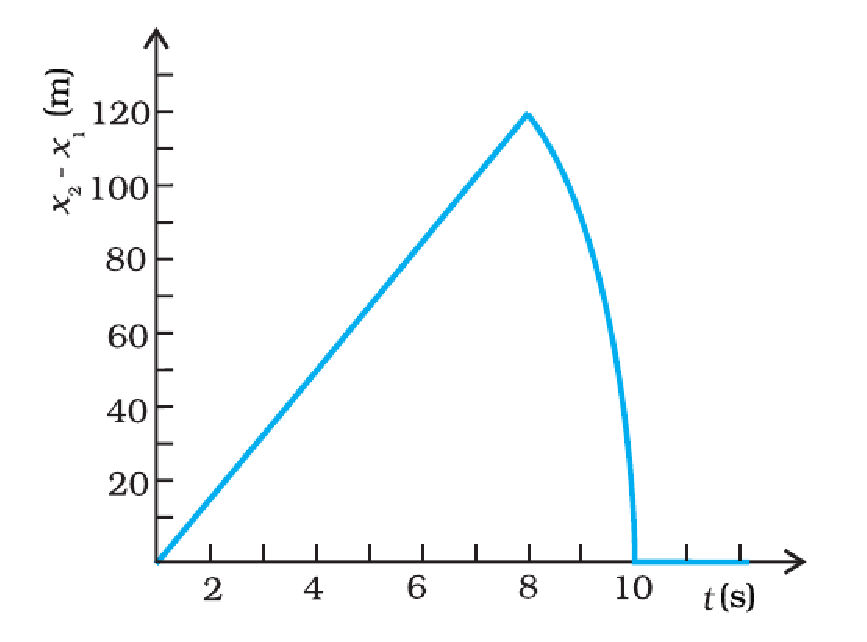
\includegraphics[width=\columnwidth]{./curves/figs/11-1-3/3.27.eps}
\caption{}
\label{fig:3.27}
\end{figure}
%
\item Figure \ref{fig:3.23} gives the x-t plot of a particle executing one-dimensional simple harmonic motion. Give the signs of position, velocity and acceleration variables of the particle at t = 0.3 s, 1.2 s, – 1.2 s.
%
\begin{figure}[!ht]
\centering
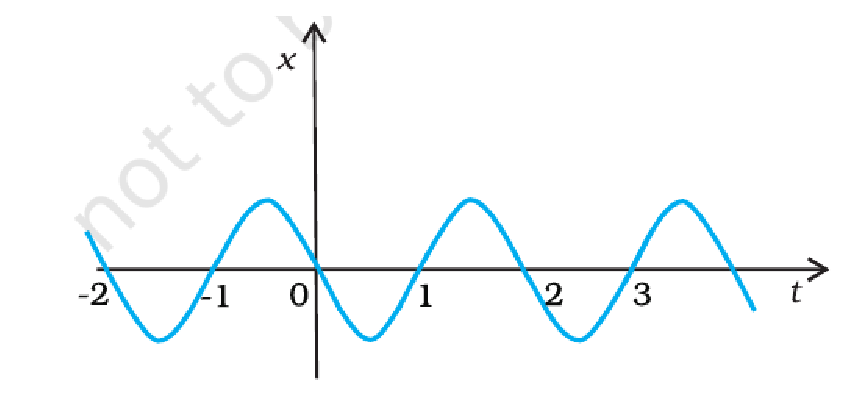
\includegraphics[width=\columnwidth]{./curves/figs/11-1-3/3.23.eps}
\caption{}
\label{fig:3.23}
\end{figure}
\item The speed-time graph of a particle moving along a fixed direction is shown in Fig. \ref{fig:3.28}. Obtain the distance traversed by the particle between (a) t = 0 s to 10 s, (b) t = 2 s to 6 s.
\begin{figure}[!ht]
\centering
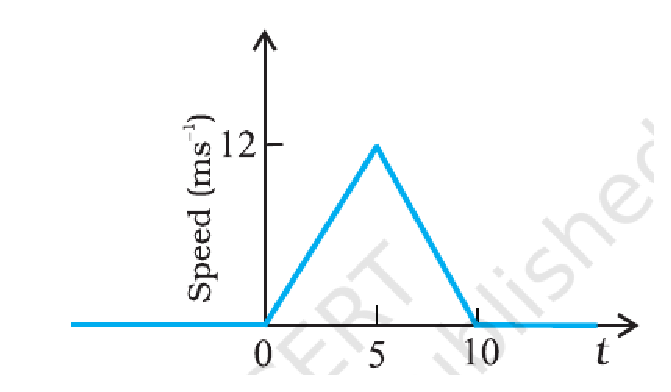
\includegraphics[width=\columnwidth]{./curves/figs/11-1-3/3.28.eps}
\caption{}
\label{fig:3.28}
\end{figure}
%
\item Figure \ref{fig:3.21} shows the x-t plot of one-dimensional motion of a particle. Is it correct to say from the graph that the particle moves in a straight line for $t < 0$ and on a parabolic path for $t >0$ ? If not, suggest a suitable physical context for this graph.
\begin{figure}[!ht]
\centering
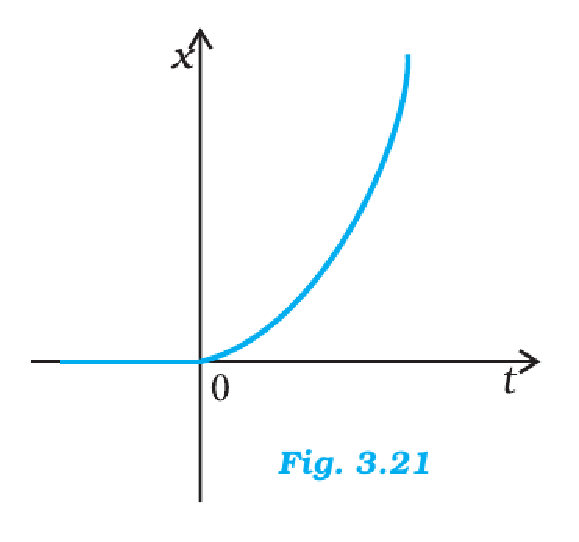
\includegraphics[width=\columnwidth]{./curves/figs/11-1-3/3.21.eps}
\caption{}
\label{fig:3.21}
\end{figure}

\end{enumerate}
 
%\section{Miscellaneous Examples}
%\renewcommand{\theequation}{\theenumi}
\begin{enumerate}[label=\arabic*.,ref=\thesubsection.\theenumi]
\numberwithin{equation}{enumi}
%
\item 
\end{enumerate}
 
%
\section{Trigonometry}
\subsection{Examples}
\renewcommand{\theequation}{\theenumi}
\begin{enumerate}[label=\arabic*.,ref=\thesubsection.\theenumi]
\numberwithin{equation}{enumi}
%
%\documentclass[journal,12pt,twocolumn]{IEEEtran}
%\usepackage{setspace}
%\usepackage{gensymb}
%\usepackage{caption}
%%\usepackage{multirow}
%%\usepackage{multicolumn}
%%\usepackage{subcaption}
%%\doublespacing
%\singlespacing
%\usepackage{csvsimple}
%\usepackage{amsmath}
%\usepackage{multicol}
%%\usepackage{enumerate}
%\usepackage{amssymb}
%%\usepackage{graphicx}
%\usepackage{newfloat}
%%\usepackage{syntax}
%\usepackage{listings}
%%\usepackage{iithtlc}
%\usepackage{color}
%\usepackage{tikz}
%\usetikzlibrary{shapes,arrows}
%
%
%
%%\usepackage{graphicx}
%%\usepackage{amssymb}
%%\usepackage{relsize}
%%\usepackage[cmex10]{amsmath}
%%\usepackage{mathtools}
%%\usepackage{amsthm}
%%\interdisplaylinepenalty=2500
%%\savesymbol{iint}
%%\usepackage{txfonts}
%%\restoresymbol{TXF}{iint}
%%\usepackage{wasysym}
%\usepackage{amsthm}
%\usepackage{mathrsfs}
%\usepackage{txfonts}
%\usepackage{stfloats}
%\usepackage{cite}
%\usepackage{cases}
%\usepackage{mathtools}
%\usepackage{caption}
%\usepackage{enumerate}
%\usepackage{tfrupee}	
%\usepackage{enumitem}
%\usepackage{amsmath}
%%\usepackage{xtab}
%\usepackage{longtable}
%\usepackage{multirow}
%%\usepackage{algorithm}
%%\usepackage{algpseudocode}
%\usepackage{enumitem}
%\usepackage{gensymb}
%\usepackage{mathtools}
%\usepackage{hyperref}
%%\usepackage[framemethod=tikz]{mdframed}
%\usepackage{listings}
%    %\usepackage[latin1]{inputenc}                                 %%
%    \usepackage{color}                                            %%
%    \usepackage{array}                                            %%
%    \usepackage{longtable}                                        %%
%    \usepackage{calc}                                             %%
%    \usepackage{multirow}                                         %%
%    \usepackage{hhline}                                           %%
%    \usepackage{ifthen}                                           %%
%  %optionally (for landscape tables embedded in another document): %%
%    \usepackage{lscape}     
%
%
%\usepackage{url}
%\def\UrlBreaks{\do\/\do-}
%
%
%%\usepackage{stmaryrd}
%
%
%%\usepackage{wasysym}
%%\newcounter{MYtempeqncnt}
%\DeclareMathOperator*{\Res}{Res}
%%\renewcommand{\baselinestretch}{2}
%\renewcommand\thesection{\arabic{section}}
%\renewcommand\thesubsection{\thesection.\arabic{subsection}}
%\renewcommand\thesubsubsection{\thesubsection.\arabic{subsubsection}}
%
%\renewcommand\thesectiondis{\arabic{section}}
%\renewcommand\thesubsectiondis{\thesectiondis.\arabic{subsection}}
%\renewcommand\thesubsubsectiondis{\thesubsectiondis.\arabic{subsubsection}}
%
%% correct bad hyphenation here
%\hyphenation{op-tical net-works semi-conduc-tor}
%
%%\lstset{
%%language=C,
%%frame=single, 
%%breaklines=true
%%}
%
%%\lstset{
%	%%basicstyle=\small\ttfamily\bfseries,
%	%%numberstyle=\small\ttfamily,
%	%language=Octave,
%	%backgroundcolor=\color{white},
%	%%frame=single,
%	%%keywordstyle=\bfseries,
%	%%breaklines=true,
%	%%showstringspaces=false,
%	%%xleftmargin=-10mm,
%	%%aboveskip=-1mm,
%	%%belowskip=0mm
%%}
%
%%\surroundwithmdframed[width=\columnwidth]{lstlisting}
%\def\inputGnumericTable{}                                 %%
%\lstset{
%%language=C,
%frame=single, 
%breaklines=true,
%columns=fullflexible
%}
% 
%
%\begin{document}
%%
%\tikzstyle{block} = [rectangle, draw,
%    text width=3em, text centered, minimum height=3em]
%\tikzstyle{sum} = [draw, circle, node distance=3cm]
%\tikzstyle{input} = [coordinate]
%\tikzstyle{output} = [coordinate]
%\tikzstyle{pinstyle} = [pin edge={to-,thin,black}]
%
%\theoremstyle{definition}
%\newtheorem{theorem}{Theorem}[section]
%\newtheorem{problem}{Problem}
%\newtheorem{proposition}{Proposition}[section]
%\newtheorem{lemma}{Lemma}[section]
%\newtheorem{corollary}[theorem]{Corollary}
%\newtheorem{example}{Example}[section]
%\newtheorem{definition}{Definition}[section]
%%\newtheorem{algorithm}{Algorithm}[section]
%%\newtheorem{cor}{Corollary}
%\newcommand{\BEQA}{\begin{eqnarray}}
%\newcommand{\EEQA}{\end{eqnarray}}
%\newcommand{\define}{\stackrel{\triangle}{=}}
%
%\bibliographystyle{IEEEtran}
%%\bibliographystyle{ieeetr}
%
%\providecommand{\nCr}[2]{\,^{#1}C_{#2}} % nCr
%\providecommand{\nPr}[2]{\,^{#1}P_{#2}} % nPr
%\providecommand{\mbf}{\mathbf}
%\providecommand{\pr}[1]{\ensuremath{\Pr\left(#1\right)}}
%\providecommand{\qfunc}[1]{\ensuremath{Q\left(#1\right)}}
%\providecommand{\sbrak}[1]{\ensuremath{{}\left[#1\right]}}
%\providecommand{\lsbrak}[1]{\ensuremath{{}\left[#1\right.}}
%\providecommand{\rsbrak}[1]{\ensuremath{{}\left.#1\right]}}
%\providecommand{\brak}[1]{\ensuremath{\left(#1\right)}}
%\providecommand{\lbrak}[1]{\ensuremath{\left(#1\right.}}
%\providecommand{\rbrak}[1]{\ensuremath{\left.#1\right)}}
%\providecommand{\cbrak}[1]{\ensuremath{\left\{#1\right\}}}
%\providecommand{\lcbrak}[1]{\ensuremath{\left\{#1\right.}}
%\providecommand{\rcbrak}[1]{\ensuremath{\left.#1\right\}}}
%\theoremstyle{remark}
%\newtheorem{rem}{Remark}
%\newcommand{\sgn}{\mathop{\mathrm{sgn}}}
%\providecommand{\abs}[1]{\left\vert#1\right\vert}
%\providecommand{\res}[1]{\Res\displaylimits_{#1}} 
%\providecommand{\norm}[1]{\left\Vert#1\right\Vert}
%\providecommand{\mtx}[1]{\mathbf{#1}}
%\providecommand{\mean}[1]{E\left[ #1 \right]}
%\providecommand{\fourier}{\overset{\mathcal{F}}{ \rightleftharpoons}}
%%\providecommand{\hilbert}{\overset{\mathcal{H}}{ \rightleftharpoons}}
%\providecommand{\system}{\overset{\mathcal{H}}{ \longleftrightarrow}}
%	%\newcommand{\solution}[2]{\textbf{Solution:}{#1}}
%\newcommand{\solution}{\noindent \textbf{Solution: }}
%\newcommand{\myvec}[1]{\ensuremath{\begin{pmatrix}#1\end{pmatrix}}}
%\providecommand{\dec}[2]{\ensuremath{\overset{#1}{\underset{#2}{\gtrless}}}}
%\DeclarePairedDelimiter{\ceil}{\lceil}{\rceil}
%%\numberwithin{equation}{section}
%%\numberwithin{problem}{subsection}
%%\numberwithin{definition}{subsection}
%\makeatletter
%\@addtoreset{figure}{section}
%\makeatother
%
%\let\StandardTheFigure\thefigure
%%\renewcommand{\thefigure}{\theproblem.\arabic{figure}}
%\renewcommand{\thefigure}{\thesection}
%
%
%%\numberwithin{figure}{subsection}
%
%%\numberwithin{equation}{subsection}
%%\numberwithin{equation}{section}
%%\numberwithin{equation}{problem}
%%\numberwithin{problem}{subsection}
%\numberwithin{problem}{section}
%%%\numberwithin{definition}{subsection}
%%\makeatletter
%%\@addtoreset{figure}{problem}
%%\makeatother
%\makeatletter
%\@addtoreset{table}{section}
%\makeatother
%
%\let\StandardTheFigure\thefigure
%\let\StandardTheTable\thetable
%\let\vec\mathbf
%%%\renewcommand{\thefigure}{\theproblem.\arabic{figure}}
%%\renewcommand{\thefigure}{\theproblem}
%
%%%\numberwithin{figure}{section}
%
%%%\numberwithin{figure}{subsection}
%
%
%
%\def\putbox#1#2#3{\makebox[0in][l]{\makebox[#1][l]{}\raisebox{\baselineskip}[0in][0in]{\raisebox{#2}[0in][0in]{#3}}}}
%     \def\rightbox#1{\makebox[0in][r]{#1}}
%     \def\centbox#1{\makebox[0in]{#1}}
%     \def\topbox#1{\raisebox{-\baselineskip}[0in][0in]{#1}}
%     \def\midbox#1{\raisebox{-0.5\baselineskip}[0in][0in]{#1}}
%
%\vspace{3cm}
%
%\title{ 
%%	\logo{
%Trigonometric Functions(Examples)
%%	}
%}
%
%\author{ G V V Sharma$^{*}$% <-this % stops a space
%	\thanks{*The author is with the Department
%		of Electrical Engineering, Indian Institute of Technology, Hyderabad
%		502285 India e-mail:  gadepall@iith.ac.in. All content in this manual is released under GNU GPL.  Free and open source.}
%	
%}	
%
%\maketitle
%
%%\tableofcontents
%
%\bigskip
%
%\renewcommand{\thefigure}{\theenumi}
%\renewcommand{\thetable}{\theenumi}
%
%
%
%\begin{enumerate}[label=\arabic*]
%\numberwithin{equation}{enumi}
\item Convert $40\degree  20^{'}$ into radian measure.
\item Convert 6 radians into radian measure.
\item Find the radius of the circle in which a central angle of $60^{o}$ intercepts an arc of length 37.4 cm (use $\pi = \frac{22}{7}$).

\item The minute hand of watch is 1.5 cm long. How far does its tip move in 40 minutes? ( $\pi = 3.14$)

\item If the arcs of the same lengths in two circles subtend angles $65^{o}$ and $110^{o}$ at the centre, find the ratio of their radii.

\item If $\cos x = -\frac{3}{5}$, x lies in the third quadrant, find the values of other five trigonometric function.

\item If $\cot x = - \frac{5}{12}$, x lies in the second quadrant, find the values of other five trigonometric function.\\ 


\item Find the value of $\sin \frac{31\pi}{3}$.\\

\item Find the value of $\cos(-1710^o)$.\\


\item Prove that 3$\sin\frac{\pi}{6}\sec\frac{\pi}{3}-4\sin\frac{5\pi}{6}\cot\frac{\pi}{4}$ = 1.\\


\item Find the value of $\sin 15^{o}$.\\

\item Find the value of $\tan\frac{13\pi}{12}$.\\


\item Prove that $\frac{\sin(x+y)}{\sin(x-y)} = \frac{\tan x + \tan y}{\tan x - \tan y}$\\


\item Show that\\
\\$\tan3x\tan2x\tan x = \tan3x-\tan2x-\tan x$.\\


\item Prove that\\
\\$\cos(\frac{\pi}{4}+x) + \cos(\frac{\pi}{4}-x) = \sqrt 2\cos x$\\


\item Prove that $\frac{\cos7x+\cos5x}{\cos7x-\cos5x} = \cot x$\\


\item Prove that $\frac{\sin5x-2\sin3x+\sin x}{\cos5x-\cos x} = \tan x$\\


\item Find the principal solutions of the equation $\sin x = \frac{\sqrt 3}{2}$.\\


\item Find the principal solutions of the equation $\tan x = -\frac{1}{\sqrt 3}$.\\


\item Find the solution of $\sin x = -\frac{\sqrt 3}{2}$.\\


\item Solve $\cos x = \frac{1}{2}$.\\


\item Solve $\tan2x=-\cot(x+\frac{\pi}{3})$.\\

\item Solve $\sin2x-\sin4x+\sin6x=0$.\\


\item Solve 2$\cos^{2}x+3\sin x=0$\\

\item If $\sin x=\frac{3}{5}, \cos y=-\frac{12}{13}$, where x and y\\ 
both lies in second quadrant, find the value of\\
$\sin(x+y)$.\\


\item Prove that\\
$\cos2x\cos\frac{x}{2}-\cos3x\cos\frac{9x}{2}=\sin5x\sin\frac{5x}{2}$\\.


\item Find the value of $\tan\frac{\pi}{8}$.\\


\item If $\tan x=\frac{3}{4}, \pi<x<\frac{3\pi}{2}$, find the value of $\sin\frac{x}{2},\cos\frac{x}{2}$ and $\tan\frac{x}{2}$\\


\item Prove that\\
$\cos^{2}x+\cos^{2}(x+\frac{\pi}{3})+\cos^{2}(x-\frac{\pi}{3})=\frac{3}{2}$\\

\end{enumerate}
%\end{document}
    
 
\subsection{Exercises}
\renewcommand{\theequation}{\theenumi}
\begin{enumerate}[label=\arabic*.,ref=\thesubsection.\theenumi]
\numberwithin{equation}{enumi}
%
%\documentclass[journal,12pt,twocolumn]{IEEEtran}
%\usepackage{setspace}
%\usepackage{gensymb}
%\usepackage{caption}
%%\usepackage{multirow}
%%\usepackage{multicolumn}
%%\usepackage{subcaption}
%%\doublespacing
%\singlespacing
%\usepackage{csvsimple}
%\usepackage{amsmath}
%\usepackage{multicol}
%%\usepackage{enumerate}
%\usepackage{amssymb}
%%\usepackage{graphicx}
%\usepackage{newfloat}
%%\usepackage{syntax}
%\usepackage{listings}
%%\usepackage{iithtlc}
%\usepackage{color}
%\usepackage{tikz}
%\usetikzlibrary{shapes,arrows}
%
%
%
%%\usepackage{graphicx}
%%\usepackage{amssymb}
%%\usepackage{relsize}
%%\usepackage[cmex10]{amsmath}
%%\usepackage{mathtools}
%%\usepackage{amsthm}
%%\interdisplaylinepenalty=2500
%%\savesymbol{iint}
%%\usepackage{txfonts}
%%\restoresymbol{TXF}{iint}
%%\usepackage{wasysym}
%\usepackage{amsthm}
%\usepackage{mathrsfs}
%\usepackage{txfonts}
%\usepackage{stfloats}
%\usepackage{cite}
%\usepackage{cases}
%\usepackage{mathtools}
%\usepackage{caption}
%\usepackage{enumerate}
%\usepackage{tfrupee}	
%\usepackage{enumitem}
%\usepackage{amsmath}
%%\usepackage{xtab}
%\usepackage{longtable}
%\usepackage{multirow}
%%\usepackage{algorithm}
%%\usepackage{algpseudocode}
%\usepackage{enumitem}
%\usepackage{mathtools}
%\usepackage{hyperref}
%%\usepackage[framemethod=tikz]{mdframed}
%\usepackage{listings}
%    %\usepackage[latin1]{inputenc}                                 %%
%    \usepackage{color}                                            %%
%    \usepackage{array}                                            %%
%    \usepackage{longtable}                                        %%
%    \usepackage{calc}                                             %%
%    \usepackage{multirow}                                         %%
%    \usepackage{hhline}                                           %%
%    \usepackage{ifthen}                                           %%
%  %optionally (for landscape tables embedded in another document): %%
%    \usepackage{lscape}     
%
%
%\usepackage{url}
%\def\UrlBreaks{\do\/\do-}
%
%
%%\usepackage{stmaryrd}
%
%
%%\usepackage{wasysym}
%%\newcounter{MYtempeqncnt}
%\DeclareMathOperator*{\Res}{Res}
%%\renewcommand{\baselinestretch}{2}
%\renewcommand\thesection{\arabic{section}}
%\renewcommand\thesubsection{\thesection.\arabic{subsection}}
%\renewcommand\thesubsubsection{\thesubsection.\arabic{subsubsection}}
%
%\renewcommand\thesectiondis{\arabic{section}}
%\renewcommand\thesubsectiondis{\thesectiondis.\arabic{subsection}}
%\renewcommand\thesubsubsectiondis{\thesubsectiondis.\arabic{subsubsection}}
%
%% correct bad hyphenation here
%\hyphenation{op-tical net-works semi-conduc-tor}
%
%%\lstset{
%%language=C,
%%frame=single, 
%%breaklines=true
%%}
%
%%\lstset{
%	%%basicstyle=\small\ttfamily\bfseries,
%	%%numberstyle=\small\ttfamily,
%	%language=Octave,
%	%backgroundcolor=\color{white},
%	%%frame=single,
%	%%keywordstyle=\bfseries,
%	%%breaklines=true,
%	%%showstringspaces=false,
%	%%xleftmargin=-10mm,
%	%%aboveskip=-1mm,
%	%%belowskip=0mm
%%}
%
%%\surroundwithmdframed[width=\columnwidth]{lstlisting}
%\def\inputGnumericTable{}                                 %%
%\lstset{
%%language=C,
%frame=single, 
%breaklines=true,
%columns=fullflexible
%}
% 
%
%\begin{document}
%%
%\tikzstyle{block} = [rectangle, draw,
%    text width=3em, text centered, minimum height=3em]
%\tikzstyle{sum} = [draw, circle, node distance=3cm]
%\tikzstyle{input} = [coordinate]
%\tikzstyle{output} = [coordinate]
%\tikzstyle{pinstyle} = [pin edge={to-,thin,black}]
%
%\theoremstyle{definition}
%\newtheorem{theorem}{Theorem}[section]
%\newtheorem{problem}{Problem}
%\newtheorem{proposition}{Proposition}[section]
%\newtheorem{lemma}{Lemma}[section]
%\newtheorem{corollary}[theorem]{Corollary}
%\newtheorem{example}{Example}[section]
%\newtheorem{definition}{Definition}[section]
%%\newtheorem{algorithm}{Algorithm}[section]
%%\newtheorem{cor}{Corollary}
%\newcommand{\BEQA}{\begin{eqnarray}}
%\newcommand{\EEQA}{\end{eqnarray}}
%\newcommand{\define}{\stackrel{\triangle}{=}}
%
%\bibliographystyle{IEEEtran}
%%\bibliographystyle{ieeetr}
%
%\providecommand{\nCr}[2]{\,^{#1}C_{#2}} % nCr
%\providecommand{\nPr}[2]{\,^{#1}P_{#2}} % nPr
%\providecommand{\mbf}{\mathbf}
%\providecommand{\pr}[1]{\ensuremath{\Pr\left(#1\right)}}
%\providecommand{\qfunc}[1]{\ensuremath{Q\left(#1\right)}}
%\providecommand{\sbrak}[1]{\ensuremath{{}\left[#1\right]}}
%\providecommand{\lsbrak}[1]{\ensuremath{{}\left[#1\right.}}
%\providecommand{\rsbrak}[1]{\ensuremath{{}\left.#1\right]}}
%\providecommand{\brak}[1]{\ensuremath{\left(#1\right)}}
%\providecommand{\lbrak}[1]{\ensuremath{\left(#1\right.}}
%\providecommand{\rbrak}[1]{\ensuremath{\left.#1\right)}}
%\providecommand{\cbrak}[1]{\ensuremath{\left\{#1\right\}}}
%\providecommand{\lcbrak}[1]{\ensuremath{\left\{#1\right.}}
%\providecommand{\rcbrak}[1]{\ensuremath{\left.#1\right\}}}
%\theoremstyle{remark}
%\newtheorem{rem}{Remark}
%\newcommand{\sgn}{\mathop{\mathrm{sgn}}}
%\providecommand{\abs}[1]{\left\vert#1\right\vert}
%\providecommand{\res}[1]{\Res\displaylimits_{#1}} 
%\providecommand{\norm}[1]{\left\Vert#1\right\Vert}
%\providecommand{\mtx}[1]{\mathbf{#1}}
%\providecommand{\mean}[1]{E\left[ #1 \right]}
%\providecommand{\fourier}{\overset{\mathcal{F}}{ \rightleftharpoons}}
%%\providecommand{\hilbert}{\overset{\mathcal{H}}{ \rightleftharpoons}}
%\providecommand{\system}{\overset{\mathcal{H}}{ \longleftrightarrow}}
%	%\newcommand{\solution}[2]{\textbf{Solution:}{#1}}
%\newcommand{\solution}{\noindent \textbf{Solution: }}
%\newcommand{\myvec}[1]{\ensuremath{\begin{pmatrix}#1\end{pmatrix}}}
%\providecommand{\dec}[2]{\ensuremath{\overset{#1}{\underset{#2}{\gtrless}}}}
%\DeclarePairedDelimiter{\ceil}{\lceil}{\rceil}
%%\numberwithin{equation}{section}
%%\numberwithin{problem}{subsection}
%%\numberwithin{definition}{subsection}
%\makeatletter
%\@addtoreset{figure}{section}
%\makeatother
%
%\let\StandardTheFigure\thefigure
%%\renewcommand{\thefigure}{\theproblem.\arabic{figure}}
%\renewcommand{\thefigure}{\thesection}
%
%
%%\numberwithin{figure}{subsection}
%
%%\numberwithin{equation}{subsection}
%%\numberwithin{equation}{section}
%%\numberwithin{equation}{problem}
%%\numberwithin{problem}{subsection}
%\numberwithin{problem}{section}
%%%\numberwithin{definition}{subsection}
%%\makeatletter
%%\@addtoreset{figure}{problem}
%%\makeatother
%\makeatletter
%\@addtoreset{table}{section}
%\makeatother
%
%\let\StandardTheFigure\thefigure
%\let\StandardTheTable\thetable
%\let\vec\mathbf
%%%\renewcommand{\thefigure}{\theproblem.\arabic{figure}}
%%\renewcommand{\thefigure}{\theproblem}
%
%%%\numberwithin{figure}{section}
%
%%%\numberwithin{figure}{subsection}
%
%
%
%\def\putbox#1#2#3{\makebox[0in][l]{\makebox[#1][l]{}\raisebox{\baselineskip}[0in][0in]{\raisebox{#2}[0in][0in]{#3}}}}
%     \def\rightbox#1{\makebox[0in][r]{#1}}
%     \def\centbox#1{\makebox[0in]{#1}}
%     \def\topbox#1{\raisebox{-\baselineskip}[0in][0in]{#1}}
%     \def\midbox#1{\raisebox{-0.5\baselineskip}[0in][0in]{#1}}
%
%\vspace{3cm}
%
%\title{ 
%%	\logo{
%Trigonometric Functions\\(Excercises)
%%	}
%}
%
%\author{ G V V Sharma$^{*}$% <-this % stops a space
%	\thanks{*The author is with the Department
%		of Electrical Engineering, Indian Institute of Technology, Hyderabad
%		502285 India e-mail:  gadepall@iith.ac.in. All content in this manual is released under GNU GPL.  Free and open source.}
%	
%}	
%
%\maketitle
%
%%\tableofcontents
%
%\bigskip
%
%\renewcommand{\thefigure}{\theenumi}
%\renewcommand{\thetable}{\theenumi}
%
%
%
%\begin{enumerate}[label=\arabic*]
%\numberwithin{equation}{enumi}
%
\item Find the radian measures corresponding to the following meausres:\\
(i) $25\degree $\\
(ii) $-47\degree 30^{'}$\\
(iii) $240\degree$\\
(iv) $520\degree$

\item Find the degree measures corresponding to the following radian measures(use $\pi$=3.14)\\
(i) $\frac{11}{16}$\\
(ii) -4\\
(iii) $\frac{5\pi}{3}$\\
(iv) $\frac{7\pi}{6}$\\

\item A wheel makes 360 revolutions in one minute. Through how many radians does it turn in one second?

\item Find the degree measure of the angle subtended at the centre of a circle of radius 100 cm by an arc of length 22 cm?

\item In a circle of diameter 40 cm, the length of a chord is 20 cm. Find the length of minor arc of the chord.

\item If in two circles, arcs of the same length subtend angles $60\degree$ and $75\degree$ at the centre, find the ratio of their radii?

\item Find the angle in radian through which a pendulum swings if its length is 75 cm and the tip describes an arc of length\\
(i) 10 cm\\
(ii) 15 cm\\
(iii) 21 cm

\item Find the values of other five trigonometric functions\\ 
1. $\cos x=-\frac{1}{2}$, x lies in third quadrant.\\
2. $\sin x= \frac{3}{5}$, x lies in second quadrant.\\
3. $\cot x= \frac{3}{4}$, x lies in third quadrant.\\
4. $\sec x= \frac{13}{5}$, x lies in fourth quadrant.\\
5. $\tan x=-\frac{5}{12}$, x lies in second quadrant.

\item Find the values of the trigonometric functions\\
1. $\sin765^{o}$\\
2. $cosec(-1410^{o})$\\
3. $\tan\frac{19\pi}{3}$\\
4. $\sin\frac{-11\pi}{3}$\\
5. $\cot\frac{-15\pi}{4}$

\item Prove that
\\1. $\sin^{2}\frac{\pi}{6}+\cos^{2}\frac{\pi}{3}-\tan^{2}\frac{\pi}{4}=-\frac{1}{2}$\\
\\2. $2\sin^{2}\frac{\pi}{6}+cosec^{2}\frac{7\pi}{6}\cos^{2}\frac{\pi}{3}=-\frac{3}{2}$\\
\\3. $\cot^{2}\frac{\pi}{6}+cosec^{2}\frac{5\pi}{6}+3\tan^{2}\frac{\pi}{6}$=6\\
\\4. $2\sin^{2}\frac{3\pi}{4}+2\cos^{2}\frac{\pi}{4}+2\sec^{2}\frac{\pi}{3}$=10\\

\item Find the value of\\
(i) $\sin75^{o}$\\
(ii) $\tan15^{o}$\\

\item Prove that \\
 $\cos(\frac{\pi}{4}-x)\cos(\frac{\pi}{4}-y)-\sin(\frac{\pi}{4}-x)\sin(\frac{\pi}{4}-y)=\sin(x+y)$\\

\item Prove that \\
\\$\frac{\tan(\frac{\pi}{4}+x)}{\tan(\frac{\pi}{4}-x)}=(\frac{1+\tan x}{1-\tan x})^{2}$\\

\item Prove that\\
\\$\frac{\cos(\pi+x)\cos(-x)}{\sin(\pi-x)\cos(\frac{\pi}{2}+x)}=\cot^{2}x$\\

\item Prove that\\
\\$\cos(\frac{3\pi}{2}+x)\cos(2\pi+x)[\cot(\frac{3\pi}{2}-x)+\cot(2\pi +x)]=1$

\item Prove that\\
\\$\sin(n+1)x\sin(n+2)x+\cos(n+1)x\cos(n+2)x=\cos x$\\

\item Prove that\\
\\$\cos(\frac{3\pi}{4}+x)-\cos(\frac{3\pi}{4}-x)=-\sqrt 2\sin x $\\

\item Prove that\\
\\$\sin^{2}6x-\sin^{2}4x=\sin2x\sin10x$\\

\item Prove that\\
\\$\cos^{2}2x-\cos^{2}6x=\sin4x\sin8x$\\

\item Prove that\\
\\$\sin2x+2\sin4x+\sin6x=4\cos^{2}x\sin4x$\\

\item Prove that\\
\\$\cot4x(\sin5x+\sin3x)= \cot x(\sin5x-\sin3x)$\\

\item Prove that\\
\\$\frac{\cos9x-\cos5x}{\sin17x-\sin3x}=-\frac{\sin2x}{\cos10x}$\\

\item Prove that\\
\\$\frac{\sin5x+\sin3x}{\cos5x+\cos3x}=\tan4x$\\

\item Prove that\\
\\$\frac{\sin x+\sin y}{\cos x+\cos y}=\tan(\frac{x-y}{2})$\\

\item Prove that\\
\\$\frac{\sin x+\sin3x}{\cos x+\cos3x}=\tan2x$\\

\item Prove that\\
\\$\frac{\sin x-\sin3x}{\sin^{2}x-\cos^{2}x}=2\sin x$\\

\item Prove that\\
\\$\frac{\cos4x+\cos3x+\cos2x}{\sin4x+\sin3x+\sin2x}=\cot3x$\\

\item Prove that\\
\\$\cot x\cot2x-\cot2x\cot3x-\cot3x\cot x=1$\\\\

\item Prove that\\
\\$\tan4x=\frac{4\tan x(1-\tan^{2}x)}{1-6\tan^{2}x+\tan^{4}x}$\\

\item Prove that\\
\\$\cos4x=1-8\sin^{2}x\cos^{2}x$\\

\item Prove that\\
\\$\cos6x=32\cos^{6}x-48\cos^{4}x+18\cos^{2}x-1$\\

\item Find the principle and general solutions of the following equations:\\
1. $\tan x=\sqrt 3$\\
2. $\sec x=2$\\
3. $\cot x=-\sqrt 3$\\
4. $cosec x=-2$\\

\item Find the general solution for each of the following equations:\\
1. $\cos4x=\cos2x$\\
2. $\cos3x+\cos x-\cos2x=0$\\
3. $\sin2x+\cos x=0$\\
4. $\sec^{2}2x=1-\tan2x$\\
5. $\sin x+\sin3x+\sin5x=0$\\

\item Prove that\\
1. 2$\cos\frac{\pi}{13}\cos\frac{9\pi}{13}+\cos\frac{3\pi}{13}+\cos\frac{5\pi}{13}=0$\\
2. $(\sin3x+\sin x)\sin x+(\cos3x-\cos x)\cos x=0$\\
3. $(\cos x+\cos y)^{2}+(\sin x-\sin y)^{2}=4\cos^{2}(\frac{x+y}{2})$\\
4. $(\cos x-\cos y)^{2}+(\sin x-\sin y)^{2}=4\sin^{2}(\frac{x-y}{2})$\\
5. $\sin x+\sin3x+\sin5x+\sin7x=4\cos x\cos2x\sin4x$\\
6. $\frac{(\sin7x+\sin5x)+(\sin9x+\sin3x)}{(\cos7x+\cos5x)+(\cos9x+\cos3x)}=\tan6x$\\
7. $\sin3x+\sin2x-\sin x=4\sin x\cos\frac{x}{2\cos\frac{3x}{2}}$\\

\item Find $\sin\frac{x}{2},\cos\frac{x}{2}$ and $\tan\frac{x}{2}$ in each of the following:\\
1. $\tan x=-\frac{4}{3}$, x in second quadrant. \\
2. $\sin x=\frac{1}{4}$, x in second quadrant.\\
3. $\cos x=-\frac{1}{3}$, x in third quadrant.\\
\end{enumerate}
%\end{document}
    
 

\section{Calculus}
\subsection{Examples}
\renewcommand{\theequation}{\theenumi}
\begin{enumerate}[label=\arabic*.,ref=\thesubsection.\theenumi]
\numberwithin{equation}{enumi}
%
%\item Find the value of each of the following polynomials at the indicated value of variables: 
%\begin{enumerate}
%\item  $q(y) = 3y^3 - 4y + 11$ at $y = 2. $
%\item  $p(t) = 4t^4+ 5t^3 - t2 + 6$ at $t = a.$
%\end{enumerate}
%%
%\item Find $p(0)$, $p(1)$ and $p(2)$ for each of the following polynomials: 
%\begin{enumerate}
%\item  $p(t) = 2 + t + 2t^2 - t^3 $
%\item $ p(x) = x^3$
%\end{enumerate}
%%
%\item Find the remainder when $x^4+x^3-2x^2+x+1$ is divided by $x-1$.
%%
%\item Check whether the polynomial $q(t) = 4t^3+4t^2-t-1$ is a multiple of $2t+1$.
%\item Examine whether $x + 2$ is a factor of $x^3 + 3x^2 + 5x + 6$ and of $2x + 4$.
%\item Find the remainder obtained on dividing $p(x) = x^3+1 $ by $x+1$.
%\item Factorize $x^3 - 23x^2 + 142x -120$.
%\item Verify that $3, -1, \frac{1}{ 3}$, are the zeroes of the cubic polynomial $p(x) = 3x^3 - 5x^2 - 11x - 3$, and then verify the relationship between the zeroes and the coefficients.
%%
%\item Show that the function $f$ given by 
%\begin{align}
%f(x) = 
%\begin{cases}
%x^3+3 & x \ne 0
%\\
%1, & x = 0
%\end{cases}
%\end{align}
%%
%is not continuous at $x = 0$.
%\item Discuss the continuity of the function $f$ defined by $f(x) = x^2+x+1$.
%\item Discuss the continuity of the function $f$ defined by $f(x) = \frac{1}{x}, x \ne 0$.
%%
%\item Show that every polynomial function is continuous.
%%
%\item Find all the points of discontinuity of the greatest integer function defined by $f(x) = [x]$, where $[x]$ denotes the greatest integer less than or equal to $x$.
%%
%\item Discuss the continuity of sine function.
%\item Show that the function defined by $f(x) = \sin (x^2 )$ is a continuous function.
%
%\item Find the slope of the tangent to the curve $y = x^3 - x$ at $x = 2$
%%
%\item Find the equation of the tangent to the curve 
%$
%y = \frac{x-7}{\brak{x-2}\brak{x-3}}
%$
%%
%\item Find the equations of the tangent and normal to the curve 
%$
%x^{\frac{2}{3}}+y^{\frac{2}{3}} 
%$
%at \myvec{1\\1}.
%\item Find the equation of the tangent to the curve 
%$
%\myvec{a \sin^3 t\\b\cos^3t}
%$
%at $t = \frac{\pi}{2}$.
%\item Find the equation of tangents to the curve $y = \cos (x + y), - 2\pi \le x \le 2\pi$
%that are parallel to the line $\myvec{1 & 2}\vec{x}= 0$.
%%
%\item Find the area bounded by the curve $y = \cos x $ between $x = 0$ and $x = 2\pi$.
%\item Find the area bounded by the curve $y = \sin x$ between $x = 0$ and $x =2\pi$.
%\item Show that the function $f$ given by 
%\begin{align}
%f(x) = x^3 - 3x^2 + 4x , x \in \vec{R}
%\end{align}
%%
%is increasing on $\vec{R}$.
%\item Prove that the function given by $f(x) = \cos x$ is
%\begin{enumerate}
%\item decreasing in $\brak{0,\pi}$.
%\item increasing in $\brak{\pi,2\pi}$ and 
%\end{enumerate}
%%
%\item Find the intervals in which the function 
%\begin{align}
%f(x)  = 4x^3-6x^2-72x+30
%\end{align}
%%
%is 
%\begin{enumerate}
%\item increasing
%\item decreasing.
%\end{enumerate}
%%
%\item Find the intervals in which the function given by 
%\begin{align}
%f(x)  = \sin x, x \in \sbrak{0,\frac{\pi}{2}}
%\end{align}
%%
%is 
%\begin{enumerate}
%\item increasing
%\item decreasing.
%\end{enumerate}
%%
%\item Find the intervals in which the function given by 
%\begin{align}
%f(x)  = \sin x + \cos x, x \in \sbrak{0,2\pi}
%\end{align}
%%
%is increasing or decreasing.
%%
%\item Find all points of local maxima and local minima of the function $f$ given by 
%%
%\begin{align}
%f(x)  = x^3-3x+3
%\end{align}
%%
%\item Find all points of local maxima and local minima of the function $f$ given by 
%%
%\begin{align}
%f(x)  = 2x^3-6x^2+6x+5
%\end{align}
%%
%\item Find the local maxima and minima of the function $f$ given by 
%%
%\begin{align}
%f(x)  = 3x^4+4x^3-12x^2+12
%\end{align}
%%
%\item Find the absolute maximum and minimum values of a function $f$ given by
%%
%\begin{align}
%f(x)  = 2x^3-15x^2+36x+1, \quad x \in \sbrak{1,5}.
%\end{align}
%%
%\item Find the absolute maximum and minimum values of a function $f$ given by
%%
%\begin{align}
%f(x)  = 12x^\frac{4}{3}-6x^{\frac{1}{3}}, \quad x \in \sbrak{1,1}.
%\end{align}
%%
%\item A car starts from a point $P$ at time $t=0$ seconds and stops at point $Q$.  The distance $x$, in metres, covered by it, in $t$ seconds is given by 
%%
%\begin{align}
%x = t^2\brak{2-\frac{t}{3}}.
%\end{align}
%%
%Find the time taken by it to reach $Q$ and also find the distance between $P$ and $Q$.
%\item A water tank has the shape of an inverted right circular cone with its axis vertical and vertex lowermost.  Its semi-vertical angle is $\tan ^{-1}(0.5)$. Water is poured
%into it at a constant rate of 5 cubic metre per hour. Find the rate at which the level of the water is rising at the instant when the depth of water in the tank is 4 m.%
%\item  A man of height 2 metres walks at a uniform speed of 5 km/h away from a lamp post which is 6 metres high. Find the rate at which the length of his shadow increases.
%%
%\item Find intervals in which the function given by 
%\begin{align}
%f(x) = \frac{3}{10}x^4 - \frac{4}{5}x^3-3x^2+\frac{36}{5} + 11 
%\end{align}
%%
%is
%%
%\begin{enumerate}
%\item decreasing 
%\item increasing 
%\end{enumerate}
%%
%\item Show that the function $f$ given by 
%%
%\begin{align}
%f(x) = \tan^{-1}\brak{\sin x + \cos x}, \quad x > 0
%\end{align}
%%
%is always an increasing function in $\brak{0,\frac{\pi}{4}}$.
%%
%\item  A circular disc of radius 3 cm is being heated. Due to expansion, its radius increases at the rate of 0.05 cm/s. Find the rate at which its area is increasing when radius is 3.2 cm.
%%
%\item An open topped box is to be constructed by removing equal squares from each corner of a 3 metre by 8 metre rectangular sheet of aluminium and folding up the sides. Find the volume of the largest such box.
%%
%\item A manufacturer can sell $x$ items at a price of $\rupee \brak{5-\frac{x}{500}}$ each.  The cost price of $x$ items is $\rupee 
%\brak{\frac{x}{5}+500}$.  Find the number of items he should sell to earn maximum profit.
%%
\item Find the derivative of the function given by $f(x) = \sin\brak{x^2}$.
\item Find the derivative of $\tan (2x + 3)$.
\item Find $\frac{dy}{dx}$ if $y + \sin y = \cos x$.
\item Find the derivative of $f(x) = \sin ^{-1}x$ assuming it exists.
\item Find the derivative of $f(x) = \tan ^{-1}x$ assuming it exists.
\item Differentiate the following with respect to $x$.
%
\begin{enumerate}
\item  $e^x$
\item  $\sin \brak{\log x}, x > 0$
\item $\cos ^{-1}\brak{e^x}$
\item $e^{\cos x}$.
\end{enumerate}
%
\item Differentiate
%
\begin{align}
\sqrt{\frac{\brak{x-3}\brak{x^2+4}}{3x^2+4x+5}}
\end{align}
\item Differentiate $a^x$ w.r.t. $x$, where $a$ is a positive constant.
\item Differentiate $x^{\sin x}, x > 0$ w.r.t. $x$.
\item Find $\frac{dy}{dx}$, if $Y^x+x^y+x^x = a^b$.
\item Find $\frac{dy}{dx}$, if $x = a \cos \theta, y = a\sin \theta$.
\item Find $\frac{dy}{dx}$, if $x = a t^2, y = 2at$.
\item Find $\frac{dy}{dx}$, if $x = a \brak{\theta+\sin \theta}, y = a\brak{1-\cos \theta}$.
\item Find $\frac{dy}{dx}$, if $x^{\frac{2}{3}}+y^{\frac{2}{3}} = a^{\frac{2}{3}}$.
\item Find $\frac{d^2y}{dx^2}$, if $y = x^3+\tan x$.
\item If $y = A \sin x + B \cos x$, then prove that  $\frac{d^2y}{dx^2} + y = 0$.
\item If $y = 3e^{2x}+2e^{3x}$, prove that $\frac{d^2y}{dx^2} - 5\frac{dy}{dx}+6y = 0$.
\item If $y = \sin ^{-1}x$, show that $\brak{1-x^2}\frac{d^2y}{dx^2} - x\frac{dy}{dx} = 0$.
\item Differentiate the following with respect to $x$.
%
\begin{enumerate}
\item  $\sqrt{3x+2}+ \frac{1}{\sqrt{2x^2+4}}$
\item  $e^{\sec^2 x} + 3\cos^{-1} x$
\item $\log_7\brak{\log x}$
\item $\cos ^{-1}\brak{\sin x}$
\item $\tan ^{-1}\brak{\frac{1}{1+\cos x}}$
\item $\sin^{-1}\brak{\frac{2^{x+1}}{1+4^x}}$
\end{enumerate}
%
\item Find $f^{\prime}(x)$ if $f(x) = \brak{\sin x}^{\sin x}$ for all $x \in \brak{0, \pi}$.
\item For a positive constant $a$, find $\frac{dy}{dx}$, where 
%
\begin{align}
y = a^{t + \frac{1}{t}}, x = \brak{t + \frac{1}{t}}^a
\end{align}
%
\item Differentiate $\sin ^2 x$ w.r.t. $e^{\cos x}$.
%\item Find the limits 
%\begin{enumerate}
%\item  $\lim_{x\to 1}x^3-x^2+1$
%\item  $\lim_{x\to 1}x\brak{x+1}$
%\item $\lim_{x\to 1}1 +x + x^2 + \dots + x^10$
%\end{enumerate}
%%
%\item Find the limits 
%\begin{enumerate}
%\item  $\lim_{x\to 1}\frac{x^2+1}{x+100}$
%\item  $\lim_{x\to 2}\frac{x^3-4x^2+4x}{x^2-4}$
%\item  $\lim_{x\to 1}\frac{x^2-4}{x^3-4x^2+4x}$
%\item  $\lim_{x\to 1}\frac{x^3-2x^2}{x^2-5x+6}$
%\item  $\lim_{x\to 1}\sbrak{\frac{x-2}{x^2-x} - \frac{1}{x^3-3x^2+2x}}$
%\end{enumerate}
%%
%\item Evaluate 
%%
%\begin{enumerate}
%\item  $\lim_{x\to 1}\frac{x^15-1}{x^10-1}$
%\item  $\lim_{x\to 2}\frac{\sqrt{1+x}}{x}$
%\end{enumerate}
%%
%\item Evaluate 
%%
%\begin{align}
%\lim_{x\to 0}\frac{\sin 4x}{\sin 2x}
%\end{align}
%
\item Find the derivative of $\sin x $ at $x = 0$.
\item Find the derivative of $f(x) = \frac{1}{x}$.
\item Find the derivative of $f(x) = 1 + x + x^2 + x^3 + \dots + x^50$ at $x = 1$.
\item Find the derivative of $f(x) = \frac{x+1}{x}$.
\item Find the derivative of $\sin x $.
\item Find the derivative of $\tan x $.
\item Find the derivative of $f(x) = \sin^2 x $.
%
\item Find the derivative of $f$ from the first principle, where $f$ is given by 
%
\begin{enumerate}
\item  $f(x) = \frac{2x+3}{x-2}$
\item  $f(x) = x + \frac{1}{x}$
\end{enumerate}
%
\item Find the derivative of $f$ from the first principle, where $f(x)$ is 
%
\begin{enumerate}
\item  $\sin x + \cos x$
\item  $x \sin x$
\end{enumerate}
%
\item Compute the derivative of 
%
\begin{enumerate}
\item  $f(x) = \sin 2x$
\item  $g(x) = \cot x$
\end{enumerate}
%
\item Find the derivative of 
%
\begin{enumerate}
\item  $\frac{x^5-\cos x}{\sin x}$
\item  $\frac{x+\cos x}{\sin x}$
\end{enumerate}
%
\item Write an an anti-derivative for each of the following functions using the method of inspection:
\begin{enumerate}
%
\item  $\cos 2x$
\item  $3x^2+4x^3$
\item  $\frac{1}{x}, x \ne 0$
%
\end{enumerate}
%%
\item Find the following integrals:
\begin{enumerate}
%
\item  $\int \frac{x^3-1}{x^2}\, dx$
\item  $\int \brak{x^{\frac{2}{3}}+1}{x^2}\, dx$
\item  $\int \brak{x^{\frac{2}{3}}+2e^x - \frac{1}{x}}{x^2}\, dx$
\end{enumerate}
%
\item Find the following integrals:
\begin{enumerate}
%
\item  $\int \brak{\sin x + \cos x} \, dx$
\item  $\int \csc x\brak{\csc  + \cot x} \, dx$
\item  $\int \frac{1-\sin x}{ \cos^2 x} \, dx$
%
\end{enumerate}
%
\item Find an anti-derivative $F$ of $f$ defined by $f(x) = 4x^3-6$, where $F(0) = 3$.
%
\item Integrate the following functions w.r.t $x$:
\begin{enumerate}
%
\item  $\sin mx$
\item  $2x\sin \brak{x^2+1}$
\item  $\frac{\tan^4 \sqrt{x} \sec^2\sqrt{x}}{\sqrt{x}}$
\item  $\frac{\sin \brak{\tan ^{-1}x}}{1+x^2}$
%
\end{enumerate}
%
\item Find the following integrals:
\begin{enumerate}
%
\item  $\int \sin^3 x \cos ^2 x \, dx$
\item  $\int \frac{\sin x}{\sin \brak{x+a}} \, dx$
\item  $\int \frac{1}{1+\tan x}  \, dx$
%
\end{enumerate}
%
\item Find 
\begin{enumerate}
%
\item  $\int \cos ^2 x \, dx$
\item  $\int \sin 2x \cos 3x\, dx$
\item  $\int \sin^3 x \, dx$
%
\end{enumerate}
%
\item Find the following integrals
\begin{enumerate}
%
\item  $\int \frac{dx}{x^2-16}$
\item  $\int \frac{dx}{\sqrt{2x-x^2}}$
%
\end{enumerate}
%
\item Find the following integrals
\begin{enumerate}
%
\item  $\int \frac{dx}{x^2-6x + 13}$
\item  $\int \frac{dx}{3x^2 + 13x -10}$
\item  $\int \frac{dx}{\sqrt{5x^2-2x}}$
%
\end{enumerate}
%
\item Find the following integrals
\begin{enumerate}
%
\item  $\int \frac{x+2}{2x^2+6x + 5}\,dx$
\item  $\int \frac{x+3}{\sqrt{5-4x-x^2}}\,dx$
%
\end{enumerate}
\item Find 
\begin{align}
\int \frac{dx}{\brak{x+1}\brak{x+2}}
\end{align}
\item Find 
\begin{align}
\int \frac{x^2+1}{x^2-5x+6}\,dx
\end{align}
%
\item Find 
\begin{align}
\int \frac{3x-2}{\brak{x+1}^2\brak{x+3}}\,dx
\end{align}
%
\item Find 
\begin{align}
\int \frac{x^2}{\brak{x^2+1}^2\brak{x^2+4}}\,dx
\end{align}
%
\item Find 
\begin{align}
\int \frac{\brak{3\sin \phi -2}\cos \phi}{5-\cos^2\phi - 4\sin \phi}\,dx
\end{align}
%
\item Find 
\begin{align}
\int \frac{x^2+x+1}{\brak{x+2}\brak{x^2+1}}\,dx
\end{align}
%
\item Find 
\begin{align}
\int x\cos x\,dx
\end{align}
%
\item Find 
\begin{align}
\int \log x\,dx
\end{align}
%
\item Find 
\begin{align}
\int xe^x\,dx
\end{align}
%
\item Find 
\begin{align}
\int \frac{x\sin^{-1}x}{\sqrt{1-x^2}}\,dx
\end{align}
%
\item Find 
\begin{align}
\int e^x \sin x\,dx
\end{align}
%
%
\item Find 
\begin{enumerate}
%
\item  $\int e^x\brak{\tan^{-1}x+\frac{1}{1+x^2}}\,dx$
\item  $\int \frac{\brak{x^2+1}e^x}{\brak{x+1}^2}\,dx$
%
\end{enumerate}
%
%
\item Find 
\begin{align}
\int \sqrt{x^2+2x+5}\,dx
\end{align}
%
\item Find 
\begin{align}
\int \sqrt{3-2x-x^2}\,dx
\end{align}
\item Find
\begin{align}
\int\cos  6x\sqrt{1+\sin6x} \,dx
\end{align}
%
\item Find
\begin{align}
\int \frac{\brak{x^4-x}^{\frac{1}{4}}}{x^5} \,dx
\end{align}
%
\item Find
\begin{align}
\int \frac{x^4}{\brak{x-1}\brak{x^2+1}} \,dx
\end{align}
%
\item Find
\begin{align}
\int \sbrak{\log \brak{\log x}}+\frac{1}{\brak{\log x}^2} \,dx
\end{align}
%
\item Find
\begin{align}
\int \sbrak{\sqrt{\cot x} + \sqrt{\tan x} }\,dx
\end{align}
%
\item Find
\begin{align}
\int \frac{\sin 2x \cos 2x }{\sqrt{9-\cos^4\brak{2x}}}\,dx
\end{align}
%
\item Verify that $y = e^{-3x}$ is a solution of the differential equation 
\begin{align}
y_2 +y_1 -6y = 0
\end{align}
%
\item Verify that $y = a\cos x + b \sin x$ is a solution of the differential equation 
\begin{align}
y_2 +y = 0
\end{align}
%
\item Form the differential equation representing the family of curves $y = a\sin\brak{x+b}$, where $a, b$ are arbitrary constants.
%
\item Find the general solution of the differential equation
%
\begin{align}
y_1  = \frac{x+1}{2-y}
\end{align}
%
\item Find the general solution of the differential equation
%
\begin{align}
y_1  = \frac{1+y^2}{1+x^2}
\end{align}
%
%
\item Show that the differential equation $\brak{x-y}y_1 = x + 2y$ is homogeneous and solve it.
\item Solve $x \cos\brak{\frac{x}{y}}y_1 = y\cos\brak{\frac{y}{x}}+x$.
\item Show that the family of curves for which the slope of the tangent at any point $\myvec{x\\y}$ on it is $\frac{x^2+y^2}{xy}$, is given by $x^2-y^2 = c$.
%
%
\item Solve 
%
\begin{align}
y_1  - y = \cos x
\end{align}
%
\item Solve 
%
\begin{align}
xy_1  + 2y = x^2
\end{align}
%
\item Solve
%
\begin{align}
y\, dx - \brak{x+2y^2}\, dy = 0
\end{align}
%
\item Solve
%
\begin{align}
y\, dx - \brak{x+2y^2}\, dy = 0
\end{align}
%
\item Verify that $y = c_1e^{ax}\cos bx + c_2 e^{ax}\sin bx$, where $c_1,c_2$ are arbitrary constants is a solution of the differential equation
%
\begin{align}
y_2 - 2ay_1 +\brak{a^2+b^2} y = 0
\end{align}
%
\item Solve
%
\begin{align}
\brak{x\,dy-y\,dx}y\sin\brak{\frac{y}{x}} = \brak{y\, dx + x\, dy}x\cos\brak{\frac{y}{x}}
\end{align}
%
\item Solve the differential equation
%
\begin{align}
\brak{\tan^{-1}x - x}\, dy = \brak{1+y^2}\, dx
\end{align}
\item The position of a particle is given by
\begin{align}
\vec{r} = \myvec{3t\\2t^2\\5}
\end{align}
where t is in seconds and the coefficients have the proper units for r to be in metres. 
\begin{enumerate}
\item  Find $\vec{v}(t)$ and $\vec{a}(t)$ of the particle. 
\item  Find the magnitude and direction of $\vec{v}(t)$ at t = 1.0 s.
\end{enumerate}
%
\item  A particle starts from origin at t = 0 with a velocity $\myvec{5.0\\0} m/s$ and moves in x-y plane under action of a force which produces a constant acceleration of $\myvec{3\\2}ms^{-2}$.
\begin{enumerate}
\item  What is the
y-coordinate of the particle at the instant its x-coordinate is 84 m ? 
\item  What is the speed of the particle at this time ?
\end{enumerate}

\end{enumerate}
 
\subsection{Exercises}
\renewcommand{\theequation}{\theenumi}
\begin{enumerate}[label=\arabic*.,ref=\thesubsection.\theenumi]
\numberwithin{equation}{enumi}
%\item Find the remainder when $x^3+3x^2+3x+1$ is divided by 
%\begin{enumerate}
%\item $x+1$
%\item $x-\frac{1}{2}$
%\item $x$
%\item $x+\pi$
%\item $5+2x$
%\end{enumerate}
%%
%\item Check whether $7+3x$ is a factor of $3x^3+7x$.
%%
%\item Determine which of the following polynomials has $(x+1)$ as a factor:
%%
%\begin{enumerate}
%\item $x^3+x^2+x+1$
%\item $x^4+x^3+x^2+x+1$
%\item $x^4+3x^3+3x^2+x+1$
%\item $x^3-x^2-\brak{2+\sqrt{2}}+\sqrt{2}$.
%\end{enumerate}
%%
%\item Determine whether $g(x)$ is a factor of $p(x)$ in each of the following cases:
%%
%\begin{enumerate}
%\item $p(x) = 2x^3+x^2-2x-1, g(x) = x+1$
%\item $p(x) = x^3+3x^2+3x+1, g(x) = x+2$
%\item $p(x) = x^4-4x^2+x+6, g(x) = x-3$
%\end{enumerate}
%%
%\item  Factorise : 
%\begin{enumerate}
%\item $x^3 – 2x^2 – x + 2 $
%\item $x^3– 3x^2 – 9x – 5 $
% \item $x^3+ 13x^2 + 32x + 20 $
%\item $2y^3+ y^2– 2y – 1$
%\end{enumerate}
%\item Find the roots of the following equations:
%\begin{enumerate}
%\item  $x - \frac{1}{x} = 3, x \ne =0 $
%\item  $ \frac{1}{x+4} - \frac{1}{x-7} = \frac{11}{30}, x\ne =-4, 7 $
%\end{enumerate}
%%
%\item Find the slope of the tangent to the curve $y = 3x^4-4x$ at $x=4$.
%\item Find the slope of the tangent to curve $y = x^3-3x+2$ at the point whose 
%x-coordinate is 2.
%\item Find the slope of the tangent to the curve $y = x^3-3x+2 $ at the point whose x-coordinate is 3.
%\item Find the slope of the normal to the curve 
%$
%\vec{x} = a \myvec{\cos^3\theta \\ \sin^{3}\theta}
%$
%at $\theta = \frac{\pi}{4}$.
%\item Find the slope of the normal to the curve 
%$
%\vec{x} =  \myvec{1-a\sin\theta \\ b\cos^{2}\theta}
%$
%at $\theta = \frac{\pi}{2}$.
%\item Find points at which the tangent to the curve $y = x^3-3x^2-9x+7$ is parallel to th x-axis.
%\item Find the point on the curve $y = x^3– 11x + 5$
%at which the tangent is $\myvec{1 & -1}\vec{x} =  11$.
%\item Find the equations of all lines having slope 0 which are tangent to the curve 
%$
%y = \frac{1}{x^2-2x+3}
%$.
%\item Find the equations of the tangent and normal to the given curves at the indicated points: 
%%
%\begin{enumerate}
%\item
%$
%y= x^4 - 6x^3+13x^2-10x+5
%$
%at \myvec{0\\5}.
%\item
%$
%y = x^4 - 6x^3+13x^2-10x+5
%$
%at \myvec{1\\3}.
%\item
%$
%y = x^3
%$
%at \myvec{1\\1}.
%\end{enumerate}
%%
%\item Show that the tangents to the curve $y = 7x^3 + 11$ at the points where $x = 2$ and $x = -2$ are parallel.
%\item Find the points on the curve $y = x^3$  at which the slope of the tangent is equal to the y-coordinate of the point.
%\item For the curve $y = 4x^3 – 2x^5$ find all the points at which the tangent passes through the origin.
%\item Find the equation of the normal at the point $\myvec{am^2 \\ am^3}$  for the curve $ay^2 = x^3$
%\item Find the equation of the normals to the curve $y = x^3+2x+6$ which are parallel to the line $\myvec{1 & 14} + 4 = 0$.
%\item Find the slope of the normal to the curve $y = 2x^2 + 3 \sin x$ at $x = 0$.
%%
%Show that the normal at any point $\theta$ to the curve $\vec{x} = \myvec{a \cos\theta + a \theta \sin\theta\\  a \sin\theta – a\theta \cos\theta}$ is at a constant distance from the origin.
%%
%\item Find the slope of the tangent to the curve $\vec{x} = \myvec{t^2+3t-8 \\ 2t^2-2t-5}$
%at the point $\myvec{2\\-1}$.
%\item Find the points on the curve $9y^2 = x^3$, where the normal to the curve makes equal intercepts with the axes.
%\item Find the area under $y = x^4, x = 1, x = 5$ and x-axis.
%%
%\item Find the area bounded by the curve $y = x^3, x =-2, x = 1$ and the x-axis.
%\item Find the area bounded by the curve $y = x \abs{x}, x = -1, x = 1$ and the x-axis.
%\item Find the area bounded by the y-axis, $y = \cos x$ and $y = \sin x$ when $0 \le x \le \frac{\pi}{2}$.\item Show that the function given by $f(x) = 3x+17$  is increasing on $\vec{R}$.
%\item Show that the function given by $f(x) = e^{2x}$  is increasing on $\vec{R}$.
%%
%%
%\item Show that the function given by 
%\begin{align}
%f(x)  = \sin x
%\end{align}
%%
%is 
%\begin{enumerate}
%\item increasing in $\brak{0,\frac{\pi}{2}}$
%\item decreasing in $\brak{\frac{\pi}{2}, \pi}$
%\end{enumerate}
%%
%%
%\item Find the intervals in which the function given by 
%\begin{align}
%f(x)  = 2x^3-3x^2 - 36x +7
%\end{align}
%%
%is 
%\begin{enumerate}
%\item increasing
%\item decreasing.
%\end{enumerate}
%%
%\item Find the intervals in which the following functions are strictly increasing or decreasing
%%
%\begin{enumerate}
%\item $\brak{x+1}^3\brak{x-3}^3$
%\item $-2x^3-9x^2-12x+1$
%\end{enumerate}
%%
%\item Show that 
%%
%\begin{align}
%y = \log \brak{1+x}-\frac{2x}{2+x}, x > -1,
%\end{align}
%%
%is an increasing function of $x$ throughout its domain.
%%
%\item Find the values of $x$ for which $y = x\brak{x-2}^2$ is an increasing function.
%%
%\item Prove that
%%
%\begin{align}
%y = \frac{4\sin \theta}{2+\cos \theta} - \theta
%\end{align}
%%
%is an incresing function of $\theta$ in $\sbrak{0,\frac{\pi}{2}}$.
%\item Prove that the logarithmic function is increasing on $\brak{0, \infty}$.
%\item Which of the following functions are decreasing on $\sbrak{0,\frac{\pi}{2}}$?
%%
%\begin{enumerate}
%\item $\cos x$
%\item $\cos 2x$
%\item $\cos 3x$
%\item $\tan x$
%\end{enumerate}
%%
%\item Find the intervals on which 
%%
%\begin{align}
%f(x) = x^{100}+\sin x -1
%\end{align}
%%
%is decreasing.
%\item Let $I$ be any interval disjoint from $\sbrak{1,-1}$.  Prove that the function $f$ given by $f(x) = x +\frac{1}{x}$ is increasing on $I$.
%\item Prove that the function $f$ given by $f(x) = \log \sin x$ is increasing on $\brak{0,\frac{\pi}{2}}$ and decreasing on $\brak{\frac{\pi}{2}, \pi}$.
%\item Prove that the function $f$ given by $f(x) = \log \abs{\cos x}$ is decreasing on $\brak{0,\frac{\pi}{2}}$ and increasing on $\brak{\frac{3\pi}{2}, 2\pi}$.
%\item Prove that the function given by $f(x) = x^3-3x^2+3x-100$ is increasing in $\vec{R}$.
%\item Find the interval(s) in which $f(x) = x^2e^{-x}$ is increasing.
%\item Find the maximum and minimum values, if any, of $g(x) = x^3+1$.
%%
%\item Find the maximum and minimum values, if any of
%the following functions given by 
%%
%\begin{enumerate}
%\item $h(x) = \sin\brak{2x} + 5$
%\item $f(x) = \abs{\sin\brak{4x} + 3}$
%\end{enumerate}
%%
%\item Find the local maximum and minima, if any, of
%the following functions.  Find also the  local maximum and local minimum values, as the case may be
%%
%\begin{enumerate}
%\item $g(x) = x^3-3x$
%\item $h(x) = \sin x +\cos x, x \in \brak{0,\frac{\pi}{2}}$
%\item $f(x) = \sin x -\cos x, x \in \brak{0,2\pi}$
%\item $f(x) = x^3-6x^2+9x+15$
%\item $g(x) = \frac{x}{2} + \frac{2}{x}, x > 0$
%\item $g(x) = \frac{1}{x^2+2}$
%\item $f(x) = x\sqrt{1-x}, 0 < x < 1$.
%\end{enumerate}
%%
%\item Prove that the following functions do not have maxima or minima:
%%
%\begin{enumerate}
%\item $f(x) = e^x$
%\item $g(x) = \log x$
%\item $h(x) = x^3+x^2+x+1$
%\end{enumerate}
%\item Find the absolute maximum and absoute minimum value of the following functions in the given intervals
%%
%\begin{enumerate}
%\item $f(x) = x^3, x \in \brak{-2,2}$
%\item $f(x) = \sin x + \cos x,  x \in \brak{0,\pi}$.
%\end{enumerate}
%%
%\item Find both the maximum value and the minimum value of 
%\begin{align}
%3x^4-8x^3+12x^2-48x+25, x \in \sbrak{0,3}.
%\end{align}
%%
%\item At what points in the interval $\sbrak{0,2\pi}$, does the function $\sin 2x$ attain its maximum value?
%\item What is the maximum value of the function $\sin x + \cos x$?
%\item Find the maximum value of $2x^3-24x+107$ in the interval $\sbrak{1,3}$.  Find the maximum value of the same function in $\sbrak{-3,1}$.
%\item It is given that at $x=1$, the function $x^4-62x^2 + ax+9$ attains its maximum value on the interval $\sbrak{0,2}$.  Find the value of $a$.
%\item Find the maximum and minimum values of $x + \sin 2x$ on $\sbrak{0, 2\pi}$.
%\item For all real values of x, the minimum value of
%\begin{align}
%\frac{1-x+x^2}{1+x+x^2}.
%\end{align}
%%
%\item Find the maximum value of 
%\begin{align}
%\sbrak{x\brak{x-1}}^{\frac{1}{3}}.
%\end{align}
%\item Using differentials, find the approximate value of each of the following
%%
%\begin{enumerate}
%\item $\brak{\frac{17}{81}}^{\frac{1}{4}}$
%\item $\brak{33}^{-\frac{1}{5}}$
%\end{enumerate}
%%
%\item Show that the function given by $f(x) = \frac{\log x}{x}$ has maximum at $x = 3$.
%\item Find the intervals in which the function $f$ given by 
%%
%\begin{align}
%f(x)  = \frac{4\sin x-2x - x\cos x}{2+\cos x}
%\end{align}
%%
%is
%%
%\begin{enumerate}
%\item increasing 
%\item decreasing 
%\end{enumerate}
%%
%\item Find the interals in which the function $f$ given by 
%%
%\begin{align}
%f(x)  = x^3 + \frac{1}{x^3}, \quad x \ne 0
%\end{align}
%%
%is
%\begin{enumerate}
%\item increasing 
%\item decreasing 
%\end{enumerate}
%%
%\item Find the absolute maximum and minimum values of the function $f$ given by 
%%
%\begin{align}
%f(x)  = \cos^2 x + \sin x , \quad x \in \sbrak{0,\pi}
%\end{align}
%%
%\item Find the points at which the function $f$ given by 
%%
%\begin{align}
%f(x)  = \brak{x-2}^4\brak{x+1}^3
%\end{align}
%%
%has
%\begin{enumerate}
%\item local maxima
%\item local minima
%\item point of inflexion
%\end{enumerate}
%%
%\item Examine the following functions for continuity.
%%
%\begin{enumerate}
%\item $f(x) = \frac{1}{x-5}$
%\item $f(x) = \frac{x^2-25}{x+5}, x \ne -5$
%\end{enumerate}
%%
%\item Prove that the function $f(x) = x^n$ is continuous at $x = n$, where $n$ is a positive integer.
%%
%\begin{enumerate}
%\item 
%$
%\begin{alignedat}[t]{2}
%f(x)=
%\begin{cases}
%x^3-3, & x \le 2,
%\\
%x^2+1, & x > 2
%\end{cases}
%\end{alignedat}
%$
%\item 
%$
%\begin{alignedat}[t]{2}
%f(x)=
%\begin{cases}
%x^10-1, & x \le 1,
%\\
%x^2, & x > 1
%\end{cases}
%\end{alignedat}
%$
%\end{enumerate}
%%
%\item Discuss the continuity of the following functions:
%%
%\begin{enumerate}
%\item 
%$
%\begin{alignedat}[t]{2}
%f(x)= \sin x + \cos x
%\end{alignedat}
%$
%\item 
%$
%\begin{alignedat}[t]{2}
%f(x)= \sin x - \cos x
%\end{alignedat}
%$
%\item 
%$
%\begin{alignedat}[t]{2}
%f(x)= \sin x \cos x
%\end{alignedat}
%$
%\end{enumerate}
%\item Discuss the continuity of the cosine, cosecant, secant and cotangent functions.
%\item Find all points of discontinuity of $f$, where 
%\begin{align}
%f(x)=
%\begin{cases}
%\frac{\sin x}{x}, & x < 0,
%\\
%x+1, & x \ge 0
%\end{cases}
%\end{align}
%\item Determine if 
%\begin{align}
%f(x)=
%\begin{cases}
%x^2\sin \brak{\frac{1}{x}}, & x \ne 0,
%\\
%0, & x = 0
%\end{cases}
%\end{align}
%%
%is a continuous function.
%\item Examine the continuity of 
%\begin{align}
%f(x)=
%\begin{cases}
%\sin x -\cos x, & x \ne 0,
%\\
%-1, & x = 0
%\end{cases}
%\end{align}
%%
%\item Find values of $k$ so that the following functions are continuous at the points indicated
%%
%\begin{enumerate}
%\item 
%$
%\begin{alignedat}[t]{2}
%\begin{cases}
%\frac{k\cos x}{\pi - 2x} & x \ne \frac{\pi}{2},
%\\
%3, & x = \frac{\pi}{2}
%\end{cases},
%\end{alignedat}
%\quad x = \frac{\pi}{2}
%$
%\item 
%$
%\begin{alignedat}[t]{2}
%\begin{cases}
%kx+1 & x \le \pi, 
%\\
%\cos x, & x > \pi,
%\end{cases}
%\quad x = \pi
%\end{alignedat}
%$
%\end{enumerate}
%%
%\item Show that the function defined by $f(x) = cos (x^2 )$ is a continuous function.
%\item  Show that the function defined by $f(x) = \abs{ cos x} $ is a continuous function. 
%\item  Examine that $sin \abs{ x}$ is a continuous function. 
%\item  Find all the points of discontinuity of $f$ defined by $f(x) = \abs{ x} – \abs{ x + 1 }$.
%%
\item Differentiate the following functions with respect to $x$
%
\begin{enumerate}
\item 
$
\sin \brak{x^2+5}
$
\item 
$
\cos \brak{\sin x}
$
\item 
$
 \sin\brak{ax+b}
$
\item 
$
\sec \brak{\tan \sqrt{x}}
$
\item 
$
\frac{\sin \brak{ax+b}}{\cos \brak{ cx+d}}
$
\item 
$
\cos x^3 \sin^2\brak{x^5}
$
\item 
$
2\sqrt{\cot \brak{x^2}}
$
\item 
$
\cos\brak{\sqrt{x}}
$
\end{enumerate}
\item Find $\frac{dy}{dx}$ in the following:
\begin{enumerate}
\item 
$
2x+3y = \sin x
$
\item 
$
2x+3y = \sin y
$
\item 
$
ax + by^2 = \cos y
$
\item 
$
xy+y^2 = \tan x + y
$
\item 
$
x^3+x^2y+xy^2+y^3 = 81
$
\item 
$
\sin^2 y + \cos xy = \kappa
$
\item 
$
\sin ^2 x + \cos ^2 y = 1
$
\item 
$
y = \sin^{-1}\brak{\frac{2x}{1+x^2}}
$
\item 
$
y = \tan^{-1}\brak{\frac{3x-x^2}{1-3x^2}}, x \in \brak{-\frac{1}{\sqrt{3}}, \frac{1}{\sqrt{3}}}
$
\item 
$
y = \cos^{-1}\brak{\frac{1-x^2}{1+x^2}}, 0 < x < 1
$
\item 
$
y = \sin^{-1}\brak{\frac{1-x^2}{1+x^2}}  < x < 1
$
\item 
$
y = \cos^{-1}\brak{\frac{2x}{1+x^2}}, - 1 < x < 1
$
\item 
$
y = \sin^{-1}\brak{2x\sqrt{1-x^2}}, -\frac{1}{\sqrt{2}} < x < \frac{1}{\sqrt{2}}
$
\item 
$
y = \sec^{-1}\brak{\frac{1}{2x^2-1}}, 0 < x < \frac{1}{\sqrt{2}}
$
\end{enumerate}
\item Differentiate the following w.r.t. $x$:
\begin{enumerate}
\item 
$
\frac{e^x}{\sin x}
$
\item 
$
e^{\sin ^{-1} x}
$
\item 
$
e^{x^3}
$
\item 
$
\sin \brak{\tan ^{-1}e^{-x}}
$
\item 
$
\log\brak{\cos e^x}
$
\item 
$
e^x + e^{x^2}+\dots+e^{x^5}
$
\item 
$
\sqrt{e^{\sqrt{x}}}, x > 0
$
\item 
$
\log\brak{\log x}, x > 1
$
\item 
$
\frac{\cos x}{\log x}, x > 0
$
\item 
$
\cos \brak{\log x + e^x}, x > 0
$
\end{enumerate}
\item Differentiate the following w.r.t. $x$
\begin{enumerate}
\item 
$
\cos x \cos 2x \cos 3x
$
\item 
$
\sqrt{\frac{\brak{x-1}\brak{x-2}}{\brak{x-3}\brak{x-4}\brak{x-5}}}
$
\item 
$
\brak{\log x}^{\cos x}
$
\item 
$
x^x - 2^{\sin x}
$
\item 
$
\brak{x+3}^2\brak{x+4}^3\brak{x+5}^4
$
\item 
$
\brak{x + \frac{1}{x}}^x+x^{1+\frac{1}{x}}
$
\item 
$
\brak{\log x}^x + \brak{\sin x}^{\cos x}
$
\item 
$
\brak{\sin x}^x +\sin^{-1}\sqrt{x}
$
\item 
$
x^{\sin x} + \brak{\sin x}^{\cos x}
$
\item 
$
x^{\cos x} + \frac{x^2+1}{x^2-1}
$
\item 
$
\brak{x \cos x}^x + \brak{x \sin x}^{\frac{1}{x}}
$
\item 
$
x^{y}+y^x = 1
$
\item 
$
y^x = x^y
$
\item 
$
\brak{\cos x}^y = \brak{\cos y}^{x}
$
\item
$
xy = e^{x-y}
$
\end{enumerate}
\item Find the derivative of the function given by 
$
f(x) = \brak{1+x}\brak{1+x^2}\brak{1+x^4}\brak{1+x^8}
$
and hence find $f^{\prime} 1$.
\item Differentiate 
$
\brak{x^2-5x+8}\brak{x^3+7x+9}
$
in three ways mentioned below:
\begin{enumerate}
\item by using product rule
\item by expanding the product to obtain a single polynomial
\item by logarithmic differentiation.
\end{enumerate}
%
Do they all give the same answer?
\item Without eliminating the parameter, find $\frac{dy}{dx}$ in the following
%
\begin{enumerate}
\item
$
x = 2at^2, y = at^4
$
\item
$
x = a\cos\theta, y =b\cos \theta
$
\item
$
x = \sin t, y =\cos t
$
\item
$
x = 4t, y = \frac{4}{t}
$
\item
$
x = \cos \theta - \cos 2\theta, y = \sin \theta  - \sin 2\theta
$
\item
$
x = a \brak{\theta - \sin \theta}, y = a\brak{1+\cos \theta}
$
\item
$
x = \frac{\sin ^3 t}{\sqrt{\cos 2t}}, y =\frac{\cos ^3 t}{\sqrt{\cos 2t}}
$
\item
$
x = a\brak{\cos t + \log \tan \frac{t}{2}} , y = a \sin t
$
\item
$
x = a\sec \theta , y = b \tan \theta
$
\item
$
x = a\brak{\cos \theta + \theta \sin \theta}, y = a\brak{\sin \theta - \theta \cos \theta}
$
\item If 
$
x = \sqrt{a^{\sin^{-1}t}}, y = \sqrt{a^{\cos^{-1}t}}
$
\end{enumerate}
%
show that $\frac{dy}{dx} = -\frac{y}{x}$.
%
\item Find the second order derivatives of the following functions
\begin{enumerate}
\item
$
x^2+3x+2
$
\item
$
x^{20}
$
\item
$
x\cos x
$
\item
$
\log x
$
\item
$
x^3\log x
$
\item
$
x^x\sin 5x
$
\item
$
e^{6x}\cos 3x
$
\item
$
\tan ^{-1}x
$
\item
$
\log \brak{\log x}
$
\item
$
\sin\brak{\log x}
$

\end{enumerate}
%
\item If $y = 5\cos x - 3 \sin x$, prove that 
$
\frac{d^2y}{dx^2} +y = 0
$
\item If $y = \cos^{-1}x$, find $\frac{d^2y}{dx^2}$ in terms of $y$.
\item If 
$
y = 3 \cos \brak{\log x} + 4\sin\brak{\log x}, 
$
show that 
$
x^2y_2+xy_1+y = 0
$
\item If 
$
y = Ae^{mx} + Be^{nx}, 
$
show that 
$
y_2 - \brak{m+n}y_1 +mny = 0.
$
\item If 
$
y = 500e^{7x} + 600 e^{-7x}, 
$
show  that 
$
y_2 = 49y
$
\item If 
$
e^y\brak{x+1} = 1,
$
show that 
$
y_2 = y_1^2
$
\item If 
$
y = \brak{\tan^{-1}x}^2, 
$
show that 
$
\brak{x^2+1}y_2+2x\brak{x^2+1}y_1 = 2
$
\item If $f: \sbrak{-5,5}\to \vec{R}$ is a differentiable function and if $f^{\prime}(x)$ does not vanish anywhere, then prove that $f(-5) \ne f(5)$.
\item Verify mean value theorem, if 
$
f(x) = x^3-5x^2-3x, x \in \sbrak{a,b}
$
where $a = 1, b = 3$.  Find all $c \in \brak{1,3}$ for which $f^{\prime}(c) = 0$
%
\item Differentiate the following functions w.r.t x
%
\begin{enumerate}
\item 
$
\brak{3x^2-9x+5}^9
$
\item 
$
\sin^3x+\cos^6x
$
\item 
$
\brak{5x}^{3\cos2x}
$
\item 
$
\sin^{-1}\brak{x\sqrt{x}}, \quad 0 \le x \le 1
$
\item 
$
\frac{\cos^{-1}\frac{x}{2}}{\sqrt{2x+7}}, -2 < x < 2
$
\item 
$
\cot^{-1}\sbrak{\frac{\sqrt{1+\sin x}+\sqrt{1-\sin x}}{\sqrt{1+\sin x}-\sqrt{1-\sin x}}}, 0 < x < \frac{\pi}{2}
$
\item 
$
\brak{\log x}^{\log x}, x > 1
$
\item 
$
\cos\brak{a\cos x + b \sin x}, 
$
for some constant $a$ and $b$.
\item 
$
\brak{\sin x - \cos x}^{\sin x - \cos x}, \quad \frac{\pi}{4}, < x < \frac{3\pi}{4}
$
\item 
$
x^x+x^a+a^x+a^a,
$
for some fixed $a > 0$ and $x > 0$.
\item 
$
x^{x^2-3}_+\brak{x-3}^{x^2}, 
$
for $x > 3$.
\end{enumerate}
\item Find $\frac{dy}{dx}$, if $y = 12\brak{1-\cos t}, x = 10\brak{t-\sin t}, -\frac{\pi}{2} < x < \frac{\pi}{2}$.
\item Find $\frac{dy}{dx}$, if 
$
y = \sin ^{-1}x + \sin^{-1}\sqrt{1-x^2}, \quad 0 < x < 1
$
\item If 
$
x\sqrt{1+y}+y\sqrt{1+x} = 0,
$
for $-1<x<1$, prove that
%
\begin{align}
\frac{dy}{dx} = -\frac{1}{\brak{1+x}^2}
\end{align}
\item If
$
\cos y = x \cos\brak{a+y}, 
$
with 
$
\cos a \ne \pm 1,
$
prove that 
$
\frac{dy}{dx}= \frac{\cos^2\brak{a+y}}{\sin a}
$
\item if 
$
x = a \brak{\cos t + t\sin t}
$
and
$
y = a \brak{\sin t - t\cos t }, 
$
find $y_2$
\item If $f(x) =\abs{x}^3$, show that $f^{''}(x)$ exists for all real $x$ and find it.
\item Using mathematical induction, prove that $\frac{d}{dx}\brak{x^n} = nx^{n-1}$ for all positive integers $n$.
\item Using the fact that 
\begin{align}
\sin\brak{x+y} = \sin x \cos y +\cos x \sin y,
\end{align}
%
show that 
\begin{align}
\cos\brak{x+y} = \cos x \cos y -\sin x \sin y
\end{align}
\item If 
\begin{align}
y = 
\mydet{
f(x) & g(x) & h(x)
\\
l &m & n
\\
a & b & c
},
\end{align}
%
prove that 
\begin{align}
\frac{dy}{dx} = 
\mydet{
f^{'}(x) & g^{'}(x) & h^{'}(x)
\\
l &m & n
\\
a & b & c
}
\end{align}
\item If $y = e^{a\cos^{-1}x}, - 1 \le x \le 1$, show that 
\begin{align}
\brak{1-x^2}y_2-xy_1-ay^2 = 0.
\end{align}
%
%\item Evaluate the following limits
%%
%\begin{enumerate}
%\item  $\lim_{x\to 4} \frac{4x+3}{x-2}$
%\item  $\lim_{x\to -1} \frac{x^10+x^5+1}{x-1}$
%\item  $\lim_{x\to 0} \frac{\brak{x+1}^5-1}{x}$
%\item  $\lim_{x\to 2} \frac{3x^2-x-10}{x^2-4}$
%\item  $\lim_{x\to 3} \frac{x^4-81}{2x^2-5x-3}$
%\item  $\lim_{x\to 0} \frac{ax+b}{cx+1}$
%\item  $\lim_{z\to 1} \frac{z^{\frac{1}{3}}-1}{z^{\frac{1}{6}}-1}$
%\item  $\lim_{x\to 1} \frac{ax^2+bx+3}{cx^2+bx+a}, \quad a+b+c \ne 0$
%\item  $\lim_{x\to 2} \frac{\frac{1}{x}+\frac{1}{2}}{x+2}$
%\item  $\lim_{x\to 0} \frac{\sin ax}{bx}$
%\item  $\lim_{x\to 0} \frac{\sin ax}{\sin bx}, \quad a,b \ne 0$
%\item  $\lim_{x\to \pi} \frac{\sin \brak{\pi-x}}{\pi \brak{\pi-x}}, \quad a,b \ne 0$
%\item  $\lim_{x\to 0} \frac{\cos x}{\pi -x}$
%\item  $\lim_{x\to 0} \frac{\cos 2x-1}{\cos x-1}$
%\item  $\lim_{x\to 0} \frac{ax + x\cos x}{b\sin x}$
%\item  $\lim_{x\to 0} x\sec x$
%\item  $\lim_{x\to 0} \frac{\sin ax + bx}{ax+\sin bx}, \quad a,b, a+b \ne 0$
%\item  $\lim_{x\to 0} \csc - \cot x$
%\item  $\lim_{x\to \frac{\pi}{2}} \frac{\tan 2x}{x-\frac{\pi}{2}}$
%\end{enumerate}
%%
%\item Find $\lim_{x\to 0} f(x)$ and $\lim_{x\to 1} f(x)$where
%\begin{align}
%f(x) = 
%\begin{cases}
%2x+3 & x \le 0
%\\
%3\brak{x+1}, & x > 0
%\end{cases}
%\end{align}
%%
%\item Let $a_1, a_2, \dots a_n$ be fixed real numbers and define a function
%\begin{align}
%f(x) = \brak{x-a_1}\brak{x-a_2}\dots \brak{x-a_n}
%\end{align}
%%
%What is $\lim_{x\to a_1} f(x)$?  For some $a \ne a_1, a_2, \dots, a_n$, compute $\lim_{x\to a} f(x)$.
%%
%\item If 
%%
%\begin{align}
%\lim_{x\to 1} \frac{f(x)-2}{x^2-1} = \pi, 
%\end{align}
%%
%evaluate $\lim_{x\to 1} f(x)$.
%%
%\item If 
%%
%\begin{align}
%f(x) = 
%\begin{cases}
%mx^2+n & x < 0
%\\
%nx +m, & 0\le x \le 1
%\\
%nx^3+m, & x > 1,
%\end{cases}
%\end{align}
%%
%for what integers $m$ and $n$ does both  $\lim_{x\to 0} f(x)$ and $\lim_{x\to 1} f(x)$ exist ?
%%

\item Find the derivative of the following functions from the first principle:
%
\begin{enumerate}
\item  $x^3-27$
\item  $\frac{1}{x^2}$
\item  $\frac{x+1}{x-1}$
\end{enumerate}
%
\item For the function 
\begin{align}
f(x) = \frac{x^100}{100} + \frac{x^99}{99} + \dots + \frac{x^2}{2} + x + 1.
\end{align}
%
prove that $f^{'}(1) = 100f^{'}(0) $.
%
\item Find the derivative of 
\begin{align}
x^n+ax^{n-1}+a^2x^{n-2}+\dots+a^n
\end{align}
%
for some fixed real number $a$.
%
\item For some constans $a$ and $b$, find the derivative of
%
\begin{enumerate}
\item  $\brak{ax^2+b}^2$
\item  $\frac{x-a}{x-b}$
\end{enumerate}
%
\item Find the derivative of $\frac{x^n-a^n}{x-a}$ for some constant $a$.
%

\item Find the derivative of 
%
\begin{enumerate}
\item  $2x-\frac{3}{4}$
\item  $\brak{5x^3+3x-1}\brak{x-1}$
\item  $x^{-3}\brak{3-4x^{-5}}$.
\item  $x^5\brak{x-6x^{-9}}$
\item  $x^{-4}\brak{3-4x^{-5}}$
\item  $\frac{2}{x+1} - \frac{x^2}{3x-1}$
\end{enumerate}
%
\item Find the derivative of $\cos x$ from the first principle.
%
\item Find the derivative of the following functions:
%
\begin{enumerate}
\item  $\sin x \cos x$
\item  $\sec x$
\item  $5\sec x + 4 \cos x$.
\item  $\csc x$
\item  $3\cot x + 5 \csc x$
\item  $5\sin x - 6 \cos x + 7$
\item  $2\tan x -7 \sec x$
\end{enumerate}
%
\item Find the derivative of the following functions:
%
\begin{enumerate}[label=(\roman*)]
\item  $\brak{-x}^{-1}$
\item  $\sin\brak{x+1}$
\item  $\cos\brak{x-\frac{\pi}{8}}$
\item  $\frac{ax+b}{cx+d}$
\item  $\brak{px+q}\brak{\frac{r}{x}+s}$
\item  $\frac{1 + \frac{1}{x}}{1-\frac{1}{x}}$
\item  $\frac{1}{ax^2+bx+c}$
\item  $\frac{ax+b}{px^2+qx+r}$
\item  $\frac{px^2+qx+r}{ax+b}$
\item  $\frac{a}{x^4}-\frac{b}{x^2}+\cos x$
\item  $4\sqrt{x}-2$
\item  $\brak{ax+b}^n$
\item  $\brak{ax+b}^n\brak{cx+d}^m$
\item  $\sin\brak{x+a}$
\item  $\csc x \cot x$
\item  $\frac{\cos x}{1+\sin x}$
\item  $\frac{\sin x + \cos x}{\sin x - \cos x}$
\item  $\frac{\sec x - 1}{\sec x + 1}$
\item  $\sin^n x$
\item  $\frac{a+b\sin x}{c+d\cos x}$
\item  $\frac{\sin\brak{x+ a}}{\cos x}$
\item  $x^4\brak{5\sin x - 3 \cos x}$
\item  $\brak{x^2+1}\cos x$
\item  $\brak{ax^2+\sin x}\brak{p +q\cos x}$
\item  $\brak{x-\tan x}\brak{x +\cos x}$
\item  $\frac{4x+5\sin x}{3x+7\cos x}$
\item  $\frac{x^2\cos \brak{\frac{\pi}{4}}}{\sin x}$
\item  $\brak{x}\brak{1+\tan x}$
\item  $\brak{x+\sec x}\brak{x -\tan x}$
\item  $\frac{x}{\sin^n x}$
%
\end{enumerate}
%
\item Find anti-derivative of each of the following functions
\begin{enumerate}
\item $\sin 2x$
\item $\cos 2x$
\item $e^{ 2x}$
\item $\brak{ ax+b}^2$
\item $\sin 2x - 4e^{2x}$
\end{enumerate}
%
\item Find the following integrals:
\begin{enumerate}
\item $\int 4e^{3x}+1,dx$
\item $\int x^2\brak{1-\frac{1}{x^2}},dx$
\item $\int\brak{\sqrt{x}-\frac{1}{\sqrt{x}}}^2\,dx$
\item $\int \brak{ax^2+bx+c},dx$
\item $\int \brak{2x^2+e^x},dx$
\item $\int \frac{x^3+5x^2-4}{x^2},dx$
\item $\int \frac{x^3-x^2+x-1}{x-1},dx$
\item $\int \brak{1-x}\sqrt{x},dx$
\item $\int \sqrt{x}\brak{3x^2+2x+3},dx$
\item $\int \brak{2x-3\cos x + e^x},dx$
\item $\int \brak{2x^2-3\sin x + 5\sqrt{x}},dx$
\item $\int \sec x\brak{\sec x + \tan x},dx$
\item $\int \frac{\sec^2 x}{\csc^2x},dx$

\end{enumerate}
%
\item Find anti-derivative of 
%
\begin{align}
\sqrt{x} + \frac{1}{\sqrt{x}}
\end{align}
%
\item If 
%
\begin{align}
\frac{d}{dx}f(x) = 4x^3 - \frac{3}{x^4}, \quad f(2) = 0
\end{align}
%
Find $f(x)$.
%
%
\item Integrate the following functions:
\begin{enumerate}[label = (\roman*)]
\item $\frac{2x}{1+x^2}$
\item $\frac{\brak{\log x}^2}{x}$
\item $\frac{1}{x+x\log x}$
\item $\sin x \sin\brak{\cos x}$
\item $\sin \brak{ax+b} \cos{a x + b}$
\item $\sqrt{ax+b}$
\item $x\sqrt{x+2}$
\item $x\sqrt{1+2x^2}$
\item $\brak{4x+2}\sqrt{x^2+x+1}$
\item $\frac{1}{x-\sqrt{x}}$
\item $\frac{x}{\sqrt{x+4}}, \quad x > 0$
\item $\brak{x^3-1}^{\frac{1}{3}}x^5$
\item $\frac{x^2}{\brak{2+3x^3}^3}$
\item $\frac{1}{x\brak{\log x}^m} \quad x > 0, m \ne 1$
\item $\frac{x}{9-4x^2}$
\item $e^{2x+3}$
\item $\frac{x}{e^{x^2}}$
\item $e^{\frac{\tan^{-1}x}{1+x^2}}$
\item $\frac{e^{2x}-1}{e^2x+1}$
\item $\frac{e^{2x}-e^{-2x}}{e^2x+e^{-2x}}$
\item $\tan^2\brak{2x-3}$
\item $\sec^2\brak{7-4x}$
\item $\frac{\sin^{-1}{x}}{\sqrt{1-x^2}}$
\item $\frac{2\cos x - 3\sin x}{6 \cos x + 4 \sin x}$
\item $\frac{1}{\cos^2 x\brak{1-\tan x}^2}$
\item $\frac{\cos \sqrt{x}}{\sqrt{x}}$
\item $\sqrt{\sin 2x}\cos 2x$
\item $\frac{\cos {x}}{\sqrt{1+\sin x}}$
\item $\cot x \log x \sin x$
\item $\frac{\sin {x}}{1+\cos x}$
\item $\frac{\sin {x}}{\brak{1+\cos x}^2}$
\item $\frac{1}{1+\cot x}$
\item $\frac{1}{1-\tan x}$
\item $\frac{\sqrt{\tan {x}}}{\sin x\cos x}$
\item $\frac{\brak{1+\log x}^2}{x}$
\item $\frac{\brak{x+1}\brak{x +\log x}^2}{x}$
\item $\frac{x^3\sin\brak{\tan^{-1}x^4}}{1+x^8}$
%
\end{enumerate}
\item Find 
$
\int \frac{10x^9+10^x\ln 10}{x^10+10^x},dx
$
\item Find 
$
\int \frac{dx}{\sin^2 x \cos^2 x},dx
$
\item Find the integrals of the following functions:
%
\begin{enumerate}[label = (\roman*)]
\item $\sin^2\brak{2x+5}$
\item $\sin 3x \cos 4x$
\item $ \cos 2x \cos 4x \cos 6x$
\item $\sin^3\brak{2x+1}$
\item $\sin^3 x \cos ^3 x$
\item $ \sin x \sin 2x \sin 3x$
\item $ \sin 4x \sin 8x$
\item $\frac{1-\cos x}{1+\cos x}$
\item $\frac{\cos x}{1+\cos x}$
\item $\sin^4 x$
\item $\cos ^4 x$
\item $\frac{\sin^2 x}{1+\cos x}$
\item $\frac{\cos 2x - \cos 2\alpha}{\cos x -\cos \alpha}$
\item $\frac{\cos x - \sin x}{1+\sin 2x}$
\item $\tan^3 {2x}\sec 2x$
\item $\tan^4 x$
\item $\frac{\sin^3 x +\cos^3 x}{\sin^2 x  \cos ^2 x}$
\item $\frac{\cos 2x +2\sin^2 x}{ \cos ^2 x}$
\item $\frac{\cos 2x}{\brak{\cos x + \sin x}^2}$
\item $\sin^{-1}\brak{\cos x}$
\item $\frac{1}{\cos\brak{x-a}\cos\brak{x-b}}$
%
\end{enumerate}
%
\item Find  
$
\frac{\sin^2 x -\cos^2 x}{\sin^2x \cos^2 x}
$
%
\item Find  
$
\frac{e^{x}\brak{1+x}}{\cos^2 \brak{e^x}}
$
\item Integrate the following functions:
%
\begin{enumerate}[label = (\roman*)]
\item $\frac{3 x^2}{x^6+1}$
\item $\frac{1}{\sqrt{1+ 4x^2}}$
\item $\frac{1}{\sqrt{1+ \brak{2-x}^2}}$
\item $\frac{1}{\sqrt{9-25x^2}}$
\item $\frac{3x}{1+2x^4}$
\item $\frac{x^2}{1-x^6}$
\item $\frac{x-1}{\sqrt{x^2-1}}$
\item $\frac{x^2}{\sqrt{x^6+a^6}}$
\item $\frac{\sec^2 x}{\sqrt{\tan^2x +4 }}$
\item $\frac{1}{\sqrt{x^2+2x+2 }}$
\item $\frac{1}{9x^2+6x+5 }$
\item $\frac{1}{\sqrt{7-6x-x^2}}$
\item $\frac{1}{\sqrt{\brak{x-1}\brak{x-2}}}$
\item $\frac{1}{\sqrt{8+3x-x^2}}$
\item $\frac{1}{\sqrt{\brak{x-a}\brak{x-b}}}$
\item $\frac{4x+1}{\sqrt{2x^2+x-3}}$
\item $\frac{x+2}{\sqrt{x^2-1}}$
\item $\frac{5x-2}{1+2x+3x^2}$
\item $\frac{6x+7}{\sqrt{\brak{x-5}\brak{x-4}}}$
\item $\frac{x+2}{\sqrt{4x-x^2}}$
\item $\frac{x+2}{\sqrt{x^2+2x+3}}$
\item $\frac{x+3}{3x^2-2x-5}$
\item $\frac{5x+3}{\sqrt{x^2+4x+10}}$
\end{enumerate}
%
\item Find 
%
$
\int \frac{dx}{x^2+2x+2}\, dx
$
%
\item Find 
%
$
\int \frac{dx}{\sqrt{9x-4x^2}}\, dx
$
%
\item Integrate the following:
\begin{enumerate}[label = (\roman*)]
\item $\frac{x}{\brak{x+1}\brak{x+2}}$
\item $\frac{1}{x^2-9}$
\item $\frac{3x-1}{\brak{x-1}\brak{x-2}\brak{x-3}}$
\item $\frac{x}{\brak{x-1}\brak{x-2}\brak{x-3}}$
\item $\frac{x}{x^2+3x+2}$
\item $\frac{1-x^2}{x\brak{1-2x}}$
\item $\frac{x}{\brak{x^2+1}\brak{x-1}}$
\item $\frac{x}{\brak{x+2}\brak{x-1}^2}$
\item $\frac{3x+5}{x^3-x^2-x+1}$
\item $\frac{2x-3}{\brak{x^2-1}\brak{2x+3}}$
\item $\frac{5x}{\brak{x^2-4}\brak{x+1}}$
\item $\frac{x^3+x+1}{x^2-1}$
\item $\frac{2}{\brak{1-x}\brak{1+x^2}}$
\item $\frac{3x-1}{\brak{x+2}^2}$
\item $\frac{1}{x^4-1}$
\item $\frac{x}{x^n+1}$
\item $\frac{\cos x}{\brak{1\sin x}\brak{2-\sin x}}$
\item $\frac{\brak{x^2+1}\brak{x^2+2}}{\brak{x^2+3}\brak{x^2+4}}$
\item $\frac{1}{e^x-1}$
\end{enumerate}
%
\item Find $\int \frac{x\, dx}{\brak{x-1}\brak{x-2}}$
\item Find $\int \frac{ dx}{x\brak{x^2+1}}$
%
\item Integrate the following functions:
\begin{enumerate}[label = (\roman*)]
\item $x\sin x$
\item $x\sin 3x$
\item $x^2e^x$
\item $x\log x$
\item $x\log 2x$
\item $x^2\log x$
\item $x\sin^{-1} x$
\item $x\tan^{-1} x$
\item $x\cos^{-1} x$
\item $\brak{\sin^{-1} x}^2$
\item $\frac{\cos^{-1} x}{\sqrt{1-x^2}}$
\item $x\sec^2 x$
\item $\tan^{-1} x$
\item $x\brak{\log x}^2$
\item $\brak{x^2+1}\log x$
\item $e^x\brak{\sin x + \cos x}$
\item $\frac{ xe^{x}}{\brak{1+x}^2}$
\item $e^x\brak{\frac{1+\sin x}{1 + \cos x}}$
\item $e^x\brak{\frac{1}{x}-\frac{1}{x^2}}$
\item $\frac{ \brak{x-3}e^{x}}{\brak{x-1}^3}$
\item $e^2x\sin x$
\item $\sin^{-1} \brak{\frac{2x}{1+x^2}}$
\end{enumerate}
%
\item Find $\int x^2e^{x^3} \, dx$
\item Find $\int e^{x}\sec x\brak{1+\tan x}\, dx$
%
\item Integrate the following functions:
\begin{enumerate}[label = (\roman*)]
\item $\sqrt{4-x^2}$
\item $\sqrt{1-4x^2}$
\item $\sqrt{x^2+4x+6}$
\item $\sqrt{x^2+4x+1}$
\item $\sqrt{1-4x-x^2}$
\item $\sqrt{x^2+4x-5}$
\item $\sqrt{1+3x-x^2}$
\item $\sqrt{x^2+3x}$
\item $\sqrt{1+\frac{x^2}{9}}$
\end{enumerate}
%
\item Integrate $\int \sqrt{1+x^2}\, dx$
\item Integrate $\int \sqrt{x^2-8x+7}\, dx$
%
\item Show that 
%
\begin{align}
\int_{0}^{a}f(x)g(x)\,dx
=2\int_{0}^{a}f(x)\,dx
\end{align}
%
if 
\begin{align}
f(x) &=f(a-x)
g(x) + g(a-x) & =4
\end{align}
%
\item Integrate the following functions:
\begin{enumerate}[label = (\roman*)]
\item $\frac{1}{x-x^3}$
\item $\frac{1}{\sqrt{x+a}+\sqrt{x+b}}$
\item $\frac{1}{x\sqrt{ax-x^2}}$
\item $\frac{1}{x^2\brak{x^4+1}^{\frac{3}{4}}}$
\item $\frac{1}{x^{\frac{1}{2}}+x^{\frac{1}{3}}}$
\item $\frac{5x}{\brak{x+1}\brak{x^2+9}}$
\item $\frac{\sin x}{\sin\brak{x-a}}$
\item $\frac{e^{5\log x}-e^{4\log x}}{e^{3\log x}-e^{2\log x}}$
\item $\frac{\cos x}{\sqrt{4-\sin^2x}}$
\item $\frac{\sin^8 x - \cos^8 x}{1-2\sin^2 x \cos^2 x}$
\item $\frac{1}{\cos\brak{x+a}\cos\brak{x+b}}$
\item $\frac{x^3}{\sqrt{1-x^8}}$
\item $\frac{e^x}{\sqrt{2+e^x}}$
\item $\frac{1}{\brak{x^2+1}\brak{x^2+4}}$
\item $\cos^3 x  e^{\log \sin x}$
\item $  e^{3\log x}\brak{x^4+1}^{-1}$
\item $\frac{1}{\sqrt{\sin^{3}x\sin\brak{x+\alpha}}}$
\item $\frac{\sin^{-1}\sqrt{x} - \cos^{-1} \sqrt{x}}{\sin^{-1}\sqrt{x} + \cos^{-1} \sqrt{x}}, x \in \sbrak{0,1}$
%
\item $\sqrt{\frac{1-\sqrt{x}}{1+\sqrt{x}}}$
\item $\frac{2+\sin 2x}{1+\cos 2x}e^{x}$
\item $\frac{x^2+x+1}{\brak{x+1}^2\brak{x+2}}$
\item $\tan^{-1}\sqrt{\frac{1-x}{1+x}}$
\item $\frac{\sqrt{x^2+1}\log\brak{x^2+1}-2\log x}{x^4}$
\end{enumerate}
\item Find $\int \frac{dx}{e^x+e^{-x}}\, dx$
\item Find $\int \frac{\cos 2x}{\sin x +\cos x}\, dx$
%
\item Verify that the given functions is a solution of the corresponding differential equation:
\begin{enumerate}[label=(\roman*)]
%
\item  $y = e^x + 1; y_2 - y_1 = 0$
\item  $y = x^2+2x+C;  y_1-2x-2 = 0$
\item  $y = \cos x+C;  y_1 + \sin x = 0$
\item  $y = \sqrt{1+x^2};  y_1 = \frac{xy}{1+x^2}$
\item  $y = Ax; xy_1 = y, x \ne 0$
\item  
$
\begin{alignedat}[t]{2}
y &= x\sin x;
\\
xy_1 &= y + x \sqrt{x^2-y^2}, \brak{x \ne 0, x > y \text{ or } x < -y}
\end{alignedat}
$
\item  $xy = \log y + C; y_1 = \frac{y^2}{1-xy}, \brak{xy \ne 1}$
\item  $y -\cos y= x; y^2y_1 + y^2 + 1 = 0$
\item  $y = \sqrt{a^2-x^2}, x \in \brak{a,-a};  x+yy_1 = 0, \brak{y \ne 0}$
%
\end{enumerate}
%
\item Form the differential equation representing the following family of curves  where $a, b$ are arbitrary constants.

\begin{enumerate}[label=(\roman*)]
%
\item  $y = ae^{3x}+be^{-2x}$
\item  $y = e^{2x}\brak{a+bx}$
\item  $y = e^{x}\brak{a\cos x +b \sin x}$
%
\end{enumerate}
%
\item Find the general solution for each of the following differntial equations
\begin{enumerate}[label=(\roman*)]
%
\item  $y_1 = \frac{1-\cos x}{1+\cos x}$
\item  $y_1 = \sqrt{4-y^2} \quad \brak{\abs{y} < 2}$
\item  $y_1 +y= 1 \quad \brak{y \ne 1}$
\item  $\sec^2 x \tan y \, dx + \sec^2 y \tan x \, dy = 0$
\item  $\brak{e^x +e^{-x}}\, dy - \brak{e^y +e^{-y}}\, dx = 0$
\item  $y_1 = \brak{1+x^2}\brak{1+y^2}$
\item  $y\log y \, dx - x \, dy = 0$
\item  $x^5y_1 = -y^5$
\item  $y_1 = \sin ^{-1} x$
\item  $e^x \tan y \, dx + \brak{1-e^x}\sec^2 y \, dy = 0$
%
\end{enumerate}
\item Find the general solution of $y_1 = e^{x+y}$
\item Solve
%
\begin{enumerate}[label = (\roman*)]
\item  $\brak{x^2+xy}dy = \brak{x^2+y^2}$
\item  $y_1 = \frac{x+y}{x}$
\item  $\brak{x-y}\,dy - \brak{x+y}\, dx = 0$
\item  $\brak{x^2-y^2}\,dx +2x y\, dy = 0$
\item  $x^2y_1 = x^2-2y^2+xy$
\item  $x\,dy - y\, dx = \sqrt{x^2+y^2}\,dx$
\item  $\cbrak{x\cos\brak{\frac{y}{x}}+y\sin\brak{\frac{y}{x}}}y\,dx = \cbrak{y\sin\brak{\frac{y}{x}}-x\cos\brak{\frac{y}{x}}}x\,dx$
\item  $xy_1 -y +x \sin \brak{\frac{y}{x}}= 0$
\item  $y\, dx +x \log \brak{\frac{y}{x}}\,dy - 2x\,dy= 0$
\item  $\brak{1+e^{\frac{x}{y}}}\, dx +e^{\frac{x}{y}}\brak{1-\frac{x}{y}}\,dy = 0$
\end{enumerate}
%
\item Solve
%
\begin{enumerate}[label = (\roman*)]
\item  $y_1 + 2y = \sin x$
\item  $y_1 + 3y = e^{-2x}$
\item  $y_1 + \frac{y}{x} = x^2$
\item  $y_1 + y\sec x  = \tan x \quad \brak{0 \le x \le \frac{\pi}{2}}$
\item  $\cos^2 x y_1 + y  = \tan x \quad \brak{0 \le x \le \frac{\pi}{2}}$
\item  $xy_1 + 2y = x^2\log x$
\item  $x\log xy_1 + y = \frac{2}{x}\log x$
\item  $\brak{1+x^2}\, dy + 2xy \, dx = \cot x \, dx$
\item  $x y_1 + y-x + xy \cot x = 0$
\item  $\brak{x+y} y_1 = 1$
\item  $y\, dx + \brak{x-y^2}\, dy = 0$
\item  $\brak{x+3y^2} y_1 = y, \quad y > 0$
\end{enumerate}
%
\item Solve 
%
\begin{align}
xy_1 -y = 2x^2
\end{align}
%
\item Solve 
%
\begin{align}
\brak{1-y^2}y_1 +xy = ay \quad \brak{-1 < y < 1}
\end{align}
%
\item For each of the exercises below, erify that the given function is a solution of the corresponding diferential equation:
%
\item Solve
%
\begin{enumerate}[label = (\roman*)]
\item  $xy = ae^x+be^{-x} + x^2; \quad xy_2+2y_1-xy+x^2-2 = 0$
\item  $y = e^x\brak{a\cos x +b\sin x}; \quad y_2-2y_1+2y = 0$
\item  $y = x\sin 3x ; \quad y_2+9y_1-6\cos 3x = 0$
\item  $x^2 = 2y^2 \log y; \quad \brak{x^2+y^2}y_1-xy = 0$
\end{enumerate}
%
\item Prove that $x^2-y^2 = c\brak{x^+y^2}^2$ is the general solution of differential equation 
%
\begin{align}
\brak{x^3-3xy^2}\, dx = \brak{y^3-3x^2y}\, dy,
\end{align}
%
where $c$ is a parameter.
%
\item Find the general solution of the differential equation
%
\begin{align}
y_1 +\sqrt{\frac{1-y^2}{1-x^2}} = 0
\end{align}
%
\item Show that the general solution of the differential equation
%
\begin{align}
y_1 +\frac{y^2+y+1}{x^2+x+1} = 0
\end{align}
%
is 
%
\begin{align}
\brak{x+y+1} = A\brak{1-x-y-2xy}, 
\end{align}
%
where $A$ is a parameter.
\item Solve
%
\begin{align}
ye^{\frac{x}{y}}\, dx = \brak{xe^{\frac{x}{y}}+y^2}\, dy
\end{align}
%
\item Solve
%
\begin{align}
\sbrak{
\frac{
e^{-2\sqrt{x}}
}
{
\sqrt{x}
}
-
\frac{y}{\sqrt{x}}
}
\end{align}
%
%
\item Solve
%
\begin{align}
\frac{y\, dx - x \, dy}{y} = 0
\end{align}
%
\item Solve
%
\begin{align}
e^{x}\, dy + \brak{ye^{x}+2x}\, dx = 0
\end{align}
\item The position of a particle is given by 
\begin{align}
\vec{r} = \myvec{3t \\-2t^2\\4}
\end{align}
where t is in seconds and the coefficients have the proper units for r to be in metres. 
\begin{enumerate}
\item  Find the $\vec{v}$ and $\vec{a}$ of the particle? 
\item  What is the magnitude and direction of velocity of the particle at t = 2.0 s ?
\end{enumerate}
\item A particle starts from the origin at t = 0 s with a velocity of $\myvec{0\\10} m/s$ and moves in the x-y plane with a constant acceleration of $\myvec{8\\2}ms^{-2}$.
\begin{enumerate}
\item  At what time is
the x- coordinate of the particle 16 m? What is the y-coordinate of the particle at that time? 
\item  What is the speed of the particle at the time ?
\end{enumerate}
\item Figure \ref{fig:5.16} shows the position-time graph of a particle of mass 4 kg. What is the 
\begin{enumerate}
\item  force on the particle for $t < 0, t > 4 s, 0 < t < 4 s$? 
\item  impulse at t = 0 and t = 4 s ? (Consider one-dimensional motion only).
\end{enumerate}
\begin{figure}[!ht]
\centering
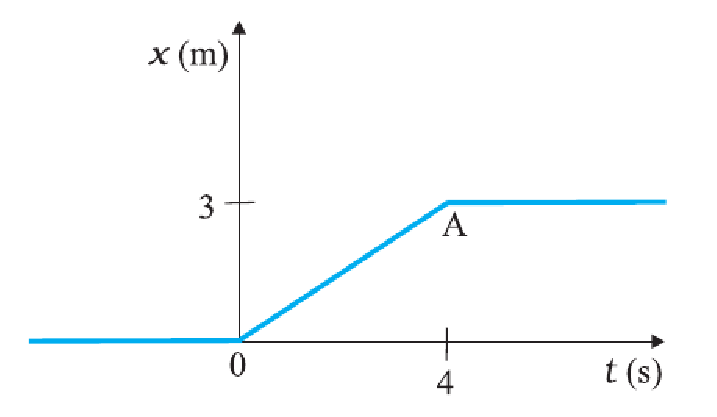
\includegraphics[width=\columnwidth]{./figs/11-1/5/5.16.eps}
\caption{}
\label{fig:5.16}
\end{figure}
\item  A body of mass 0.5 kg travels in a straight line with velocity $v =a x^{\frac{3}{2}}$ where $a = 5 m^{–1/2}s^{-1}$ .
What is the work done by the net force during its displacement from x = 0 to x = 2 m ?
\end{enumerate}
 
\section{Miscellaneous Exercises}
\renewcommand{\theequation}{\theenumi}
\begin{enumerate}[label=\arabic*.,ref=\thesubsection.\theenumi]
\numberwithin{equation}{enumi}

\item If a parabolic reflector is 20 cm in diameter and 5 cm deep, find the focus. 
\item An arch is in the form of a parabola with its axis vertical. The arch is 10 m high and 5 m wide at the base. How wide is it 2 m from the vertex of the parabola?
\item The cable of a uniformly loaded suspension bridge hangs in the form of a parabola. The roadway which is horizontal and 100 m long is supported by vertical wires attached to the cable, the longest wire being 30 m and the shortest being 6 m. Find the length of a supporting wire attached to the roadway 18 m from the middle.
\item An arch is in the form of a semi-ellipse. It is 8 m wide and 2 m high at the centre. Find the height of the arch at a point 1.5 m from one end.
\item A rod of length 12 cm moves with its ends always touching the coordinate axes. Determine the equation of the locus of a point P on the rod, which is 3 cm from the end in contact with the x-axis.
\item Find the area of the triangle formed by the lines joining the vertex of the parabola $x^2= 12y$ to the ends of its latus rectum.
\item A man running a racecourse notes that the sum of the distances from the two flag posts from him is always 10 m and the distance between the flag posts is 8 m. Find the equation of the posts traced by the man.
\item An equilateral triangle is inscribed in the parabola $y^2 = 4 ax$, where one vertex is at the vertex of the parabola. Find the length of the side of the triangle.
%
%
 \item Prove that the curves $x = y^2$ and $kx=y$ cut at right angles if $8k^2 = 1$

\item Find the equations of the tangent and normal to the parabola 
$y^2 = 4ax$ at the point $\myvec{at^2\\2at}$.
\item Find the equations of the tangent and normal to the hyperbola 
$
\vec{x}^T\myvec{\frac{1}{a^2} & 0 \\ 0 & -\frac{1}{b^2}}\vec{x} = 1
$
at the point $\myvec{x_0\\ y_0 }$.
\item  Find the area of the smaller part of the circle $\vec{x}^\vec{x}=a^2$ cut off by the line $x = \frac{a}{\sqrt{2}}$.
\item Find the area enclosed between the parabola $y^2=4ax$ ad the line $y = mx$.
\item The focus of a parabolic mirror is at a distance of 5 cm from its vertex. If the mirror is 45 cm deep, find the distance AB .
\item A beam is supported at its ends by  supports which are 12 metres apart. Since the load is concentrated at its centre, there is a deflection of 3 cm at the centre and the deflected beam is in the shape of a parabola. How far from the centre is the deflection 1 cm?
\item 19 A rod AB of length 15 cm rests in between two coordinate axes in such a way that the end point $\vec{A}$ lies on x-axis and end point $\vec{B}$ lies on y-axis. A point $\vec{P}$ is taken on the rod in such a way that $AP$ = 6 cm. Show that the locus of P is an ellipse
%
\item Find the area of the parabola $y^2 = 4ax$ bounded by its latus rectum.
\item Find the rate of change of the area of a circle per second with respect to its radius when $r = 5$cm.
\item The volume of a cube is increasing at a rate of 9 cu cm per second.  How fast is the surface area increasing when the length of an edge is 10 cm?
\item A stone is dropped into a quiet lake and waves move in circles at a speed of 4cm per second. At the instant, when the radius of the circular wave is 10 cm, how fast is the enclosed area increasing?
\item The length $x$ of a rectangle is decreasing at the rate of 3 cm/minute and the width $y$ is increasing at the rate of 2cm/minute. When x =10cm and y =6cm, find the rates of change of (a) the perimeter and (b) the area of the rectangle.
\item The total cost $C(x)$ in Rupees, associated with the production of $x$ units of an item is given by
$C(x) = 0.005 x^3 – 0.02 x^2 + 30x + 5000$
Find the marginal cost when 3 units are produced, where by marginal cost we mean the instantaneous rate of change of total cost at any level of output.
\item The total revenue in Rupees received from the sale of x units of a product is given by $R(x) = 3x^2
+ 36x + 5$. Find the marginal revenue, when $x = 5$, where by marginal revenue we mean the rate of change of total revenue with respect to the number of items sold at an instant.
\item Find the rate of change of the area of a circle with respect to its radius $r$ when (a) $r = 3$ cm
(b) $r = 4$ cm
\item  The volume of a cube is increasing at the rate of 8 $cm^3$/s. How fast is the surface area increasing when the length of an edge is 12 cm?

\item The radius of a circle is increasing uniformly at the rate of 3 cm/s. Find the rate at which the area of the circle is increasing when the radius is 10 cm.
\item An edge of a variable cube is increasing at the rate of 3 cm/s. How fast is the volume of the cube increasing when the edge is 10 cm long?
\item A stone is dropped into a quiet lake and waves move in circles at the speed of 5 cm/s. At the instant when the radius of the circular wave is 8 cm, how fast is the enclosed area increasing?
%
\item The radius of a circle is increasing at the rate of 0.7 cm/s. What is the rate of increase of its circumference?
\item The length $x$ of a rectangle is decreasing at the rate of 5 cm/minute and the width $y$ is increasing at the rate of 4 cm/minute. When $x = 8$cm and $y = 6$cm, find the rates of change of (a) the perimeter, and (b) the area of the rectangle.
\item A balloon, which always remains spherical on inflation, is being inflated by pumping in 900 cubic centimetres of gas per second. Find the rate at which the radius of the balloon increases when the radius is 15 cm.
\item A balloon, which always remains spherical has a variable radius. Find the rate at which its volume is increasing with the radius when the later is 10 cm.
\item A ladder 5 m long is leaning against a wall. The bottom of the ladder is pulled along the ground, away from the wall, at the rate of 2cm/s. How fast is its height on the wall decreasing when the foot of the ladder is 4 m away from the wall ?
\item A particle moves along the curve $6y = x3 +2$. Find the points on the curve at which the y-coordinate is changing 8 times as fast as the x-coordinate.
\item The radius of an air bubble is increasing at the rate of 12cm/s.   At what rate is the
volume of the bubble increasing when the radius is 1 cm?
\item A balloon, which always remains spherical, has a variable diameter $\frac{3}{ 2}2x+1$.
Find the rate of change of its volume with respect to $x$.
\item Sand is pouring from a pipe at the rate of 12 cm$^3$/s. The falling sand forms a cone
on the ground in such a way that the height of the cone is always one-sixth of the radius of the base. How fast is the height of the sand cone increasing when the height is 4 cm?
\item The total cost $C (x)$ in Rupees associated with the production of $x$ units of an item is given by
$C (x) = 0.007x^3 – 0.003x^2 + 15x + 4000$. Find the marginal cost when 17 units are produced.
\item The total revenue in Rupees received from the sale of $x$ units of a product is given by
$R (x) = 13x2 + 26x + 15$.
Find the marginal revenue when x = 7. 
\item Find the rate of change of the area of a circle with respect to its radius r at r = 6 cm.
\item The total revenue in $\rupee$ received from the sale of x units of a product is given by $R(x) = 3x^2+ 36x + 5$. Find the marginal revenue, when $x = 15$.
%
\item For what vaues of $a$ the function given by $f(x) = x^2+ax+1$ is increasing on $\sbrak{1,2}$?
%
\item Let $AP$ and $BQ$ be two vertical poles at points $A$ and $B$ respectively.  If $AP = 16$m, $BQ = 22$m, and $AB=20$m, then find the distance of a point $R$ on $AB$ from the point $A$ such that $RP^2+RQ^2$ is minimum.
\item  If length of three sides of a trapezium other than base are equal to 10cm, then find the area of the trapezium when it is maximum.
%
\item Prove that the radius of the right circular cylinder of greatest curved surface area which can be inscribed in a given cone is half of that of the cone.
%
\item Find two positive numbers x and y such that $x + y = 60$ and $xy^3$
is maximum.
\item  Find two positive numbers x and y such that their sum is 35 and the product $x^2 y^5$ is a maximum.
\item A square piece of tin of side 18 cm is to be made into a box without top, by cutting a square from each corner and folding up the flaps to form the box. What should be the side of the square to be cut off so that the volume of the box is the maximum possible.
\item  A rectangular sheet of tin 45 cm by 24 cm is to be made into a box without top, by cutting off square from each corner and folding up the flaps. What should be the side of the square to be cut off so that the volume of the box is maximum ?
\item  Show that of all the rectangles inscribed in a given fixed circle, the square has the maximum area.
\item  Show that the right circular cylinder of given surface and maximum volume is such that its height is equal to the diameter of the base.
\item  Of all the closed cylindrical cans (right circular), of a given volume of 100 cubic centimetres, find the dimensions of the can which has the minimum surface area.
\item  A wire of length 28 m is to be cut into two pieces. One of the pieces is to be made into a square and the other into a circle. What should be the length of the two pieces so that the combined area of the square and the circle is minimum?
\item  Prove that the volume of the largest cone that can be inscribed in a sphere of radius $R$ is
$\frac{8}{ 27}$ of the volume of the sphere.
\item  Show that the right circular cone of least curved surface and given volume has an altitude equal to $\sqrt{2}$ time the radius of the base.
\item  Show that the semi-vertical angle of the cone of the maximum volume and of given slant height is
$\tan^{-1} \sqrt{2}$.

\item  Show that semi-vertical angle of right circular cone of given surface area and maximum volume is $\sin^{-1} \frac{1}{ 3}$
.
\item Show that the altitude of the right circular cone of maximum volume that can be inscribed in a sphere of radius $r$ is $\frac{4r}{ 3}$.
\item Show that height of the cylinder of greatest volume which can be inscribed in a right circular cone of height $h$ and semi vertical angle $\alpha $ is one-third that of the cone and the greatest volume of cylinder is $\frac{4}{27} \pi h^3 \tan^2\alpha $.
\item A cylindrical tank of radius 10 m is being filled with wheat at the rate of 314 cubic metre per hour. Find the rate at which the depth of the wheat is increasing.
\item Let $f$ be a function defined on $\sbrak{a,b}$ such that $f^{\prime}(x) = 0,$ for all $x \in \brak{a,b}$.  Then prove that $f$ is an increasing function on $\brak{a,b}$.
%
\item Prove that every rational function is continuous.
\item Prove that the function defined by $f(x) = \tan x$ is a continuous function.
\item  A cyclist is riding with a speed of 27 km/h. As he approaches a circular turn on the road of radius 80 m, he applies brakes and reduces his speed at the constant rate of 0.50 m/s every second. What is the magnitude and direction of the net acceleration of the cyclist on the circular turn ?
\item A block of mass m = 1 kg, moving on a horizontal surface with speed $v_i
= 2 m s^{-1}$
enters a rough patch ranging from x = 0.10 m to x = 2.01 m. The retarding force $F_r$
on the block in this range is inversely proportional to x over this range,
%
\begin{align}
 F = 
\begin{cases}
 0 & x < 0
\\
-\frac{k}{ x}, & 0.1 < x < 2.01 
\\
0 & x > 2.01 
\end{cases}
\end{align}
%
where k = 0.5 J. What is the final kinetic energy and speed $v_f$
crosses this patch ?
\item The potential energy function for a particle executing linear simple harmonic motion is given by $V(x) = \frac{kx^2}{2}$, where k is the force constant of the oscillator. For $k = 0.5 N m^{-1}$
,
the graph of $V(x)$ versus $x$ is shown in Fig. \ref{fig:6.12}. Show that a particle of total energy 1 J moving under this potential must ‘turn back’ when it reaches $x = \pm 2$ m.
\begin{figure}[!ht]
\centering
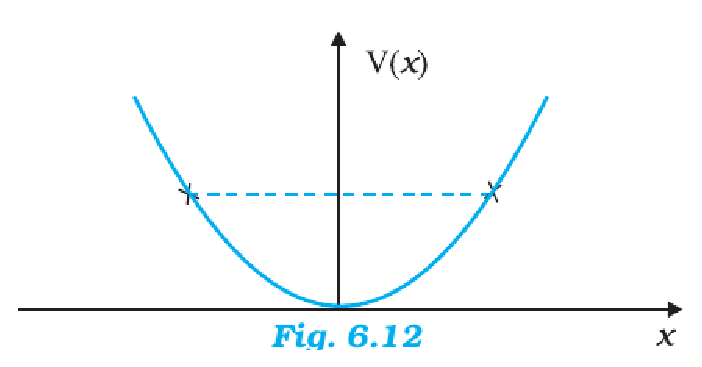
\includegraphics[width=\columnwidth]{./figs/11-1/6/6.12.eps}
\caption{}
\label{fig:6.10}
\end{figure}

\end{enumerate}
 

\end{document}


